\section{Two-Particle Correlation Function}
\makeatletter
\DeclareRobustCommand{\textsupsub}[2]{{%
  \m@th\ensuremath{%
    ^{\mbox{\fontsize\sf@size\z@#1}}%
    _{\mbox{\fontsize\sf@size\z@#2}}%
  }%
}}
\makeatother

In this analysis with ALEPH open data, charged particles with transverse momentum between 0.1 and 4.0 GeV/$c$ 
are selected for the correlation function analysis. High multiplicity events are sampled using the total number of selected proton, 
pions and kaons (hadron multiplicity $N$) in each event. The first step in extracting the correlation function was to divide the sample 
into bins in the hadron multiplicity. For each hadron multiplicity class, ``trigger" particles are defined as charged hadrons in the selected transverse momentum range (0.1 and 4.0 GeV/$c$). Particle pairs are then formed by associating every trigger particle with the remaining charged hadrons in the same $p_{\rm T}$ interval as the trigger particle. The per-trigger-particle associated yield is defined as:
\begin{eqnarray}
\label{eq:associatedyield}
\frac{1}{N_{\rm trig}}\frac{\rm d^2N^{pair}}{d\Delta\eta  \rm d\Delta\phi}= B(0,0) \times \frac{S(\Delta\eta, \Delta\phi)}{B(\Delta\eta, \Delta\phi)}
\end{eqnarray}
where $N_{trig}$ is the number of trigger particles in the event, $\Delta\eta$ and $\Delta\phi$ are the differences in $\eta$ and $\phi$ of the pair. The signal distribution, $S(\Delta\eta, \Delta\phi)$, 
is the per-trigger-particle yield of particle pairs in the same event: 
\begin{eqnarray}
\label{eq:S}
S(\Delta\eta,\Delta\phi) = \frac{1}{N_{trig}}\frac{\rm d^2 N^{\rm same}}{\rm d\Delta\eta \rm d\Delta\phi}
\end{eqnarray}
The mixed-event background distribution, used to account for random combinatorial background, is defined as 
\begin{eqnarray}
\label{eq:B}
B(\Delta\eta,\Delta\phi) = \frac{1}{N_{trig}}\frac{\rm d^2 N^{\rm mix}}{\rm d\Delta\eta \rm d\Delta\phi}
\end{eqnarray}
and is constructing by pairing the trigger particles from two random events in the same hadron multiplicity interval.
The symbol $N^{mix}$ denotes the number of pairs taken from the mixed event, while $B(0,0)$ represents the mixed-event associated yield for both particles of the pair going in the same direction and thus having full pair acceptance. Therefore, 
the ratio $B(0,0)/B(\Delta\eta,\Delta\phi)$ represents the pair-acceptance correction factor used to derive the corrected per-trigger-particle
associated yield distribution.  The signal and background distributions are first calculated for each event and then averaged over all the events within the track multiplicity class. 

In the full data analysis, a matching between particles and the primary vertex should be performed so that the studies are done with primary hadrons from a single primary vertex. This matching requirement is not yet included in this preliminary analysis due to the limited information in the Belle open data. 

\begin{table*}[h!]\centering
\ra{1.3}

\begin{tabular}{cccccccc}\toprule
Axis & ${p_{T}}$ & $|\eta|$ & $\theta$ & ${p}$ & $|dxy|$ & $|dz|$ & nTPC\\
\midrule
\rowcolor{black!20} {0} Beam & $\geq$0.4 & $<$1.8 & [20,160] & $>$0.2 & $<$3.0 & $<$5.0 & $\geq$4.0 \\
{2} Thrust & $\geq$0.4 & $<$5.0 & $\theta$ & ${p}$ & $|dxy|$ & $|dz|$ & nTPC \\
\rowcolor{black!20} {3} WTA & $\geq$0.4 & $<$5.0 & $\theta$ & ${p}$ & $|dxy|$ & $|dz|$ & nTPC \\
\bottomrule
\end{tabular}
\caption{Track cuts for Beam, Thrust, and WTA axes.}
\end{table*}

\begin{table*}[h!]\centering
\ra{1.3}

\begin{tabular}{cccccc}\toprule
Axis & WW & ${p^{miss}}$ & 2-Jet ${p^{rel}}$ & 3rd-Jet ${p^{rel}_{1,2}}$ &
$N_{trk}$ \\
\midrule
\rowcolor{black!20} {0} Beam & WW & $\leq$20 & 0.1 & 0.03 & $>$1 \\
{2} Thrust & WW & missP & 2-Jet & 3rd Jet & N trk \\
\rowcolor{black!20} {3} WTA & WW & missP & 2-Jet & 3rd Jet & N trk \\
\bottomrule
\end{tabular}
\caption{Event cuts for Beam, Thrust, and WTA axes.}
\end{table*}

Two particle correlation functions for the LEP1 and LEP2 data sets analyzed in the beam, thrust, and winner-take-all (WTA) axes are shown below. The first row contains events with nTrk $<$ 20, the second with 20 $\leq$ nTrk $<$ 30, and third with 30 $\leq$ nTrk. The first column contains Anthony's analysis, the second contains Austin's cross-check, and the third contains the ratio of the two.

%%%% file 1 is Austin and file 2 is Anthony in the below plots outputed by TPCPlots.cc %%%%

%%%%%%%%%%% LEP1 %%%%%%%%%%%
\begin{figure}[h!]
\centering
\subfloat{\label{sfig:a}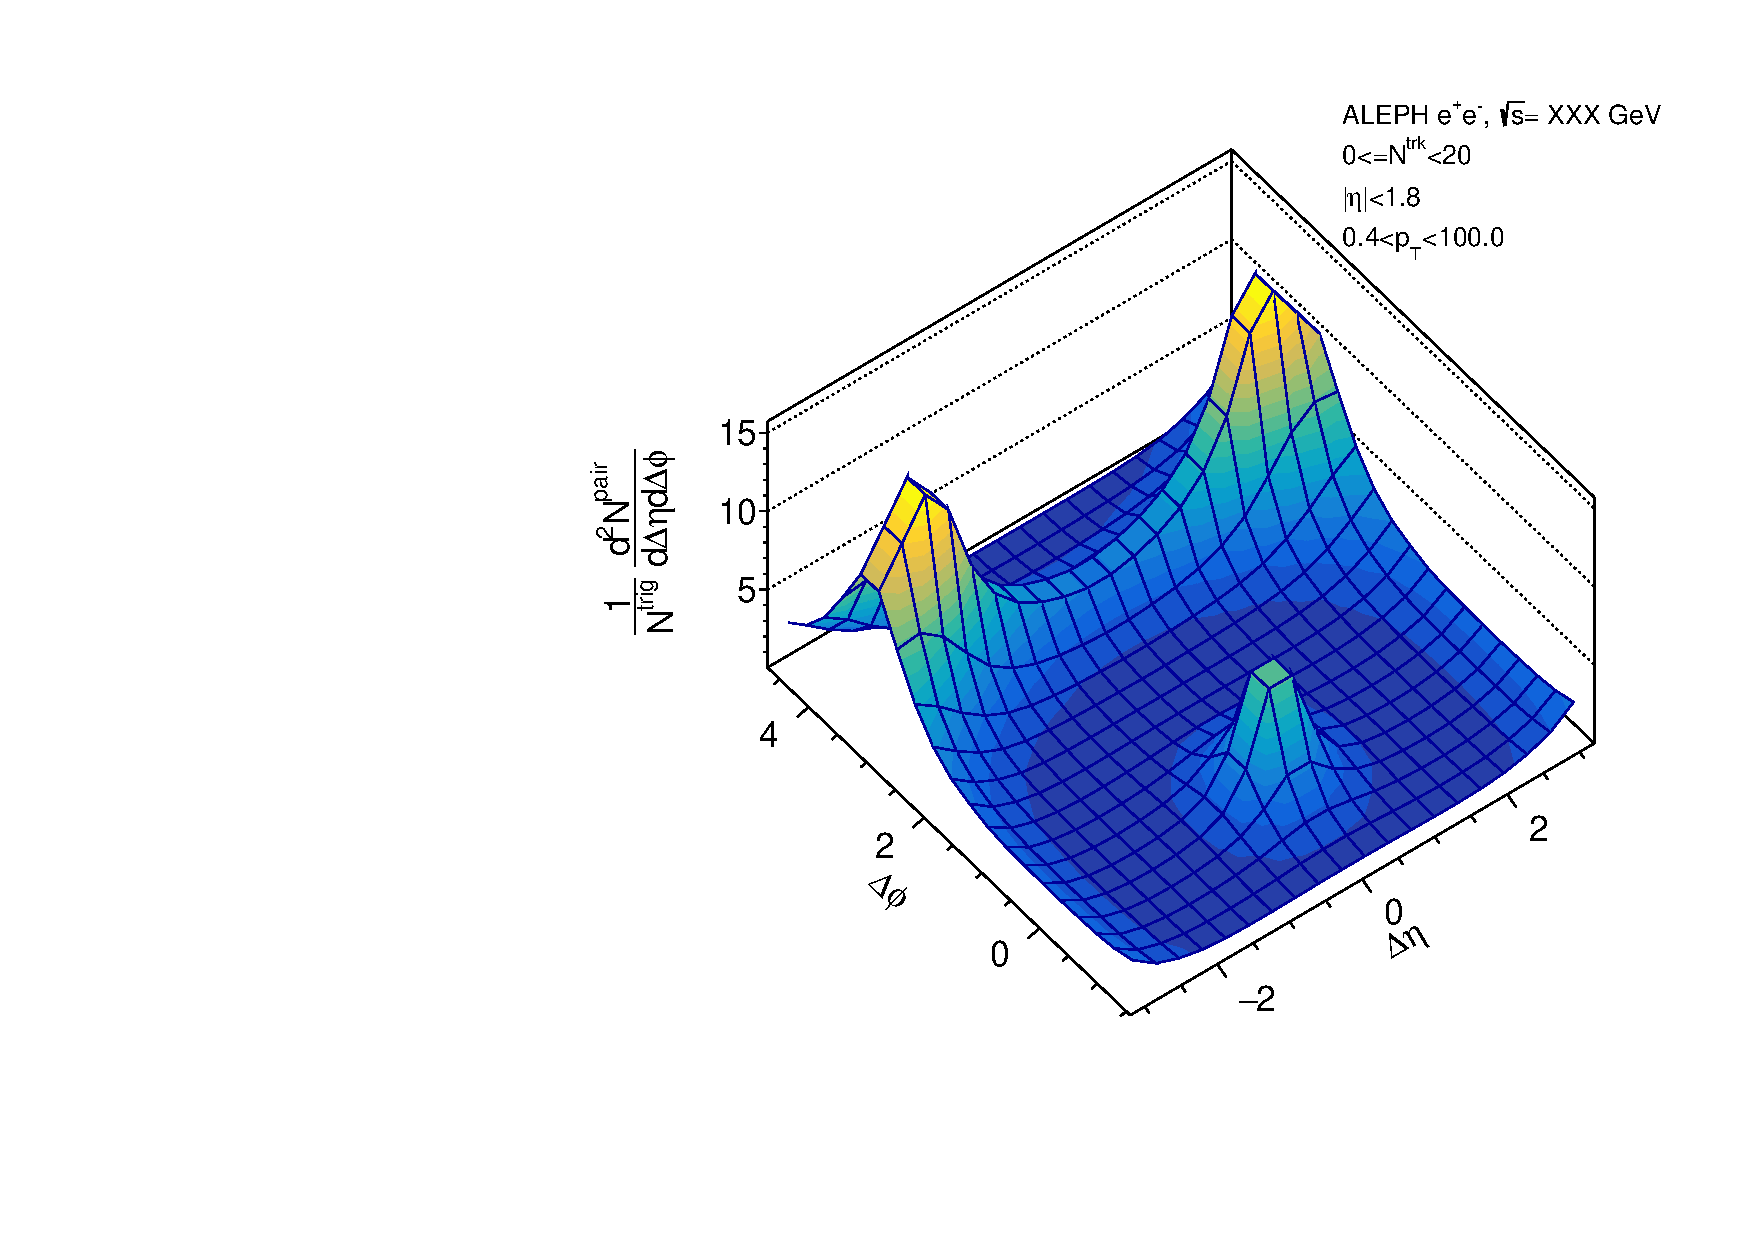
\includegraphics[width=.32\textwidth]{images/TwoParticleCorrelation/LEP1_BEAM/LEP1_BEAM_ratio2_0_20.pdf}}\hfill
\subfloat{\label{sfig:b}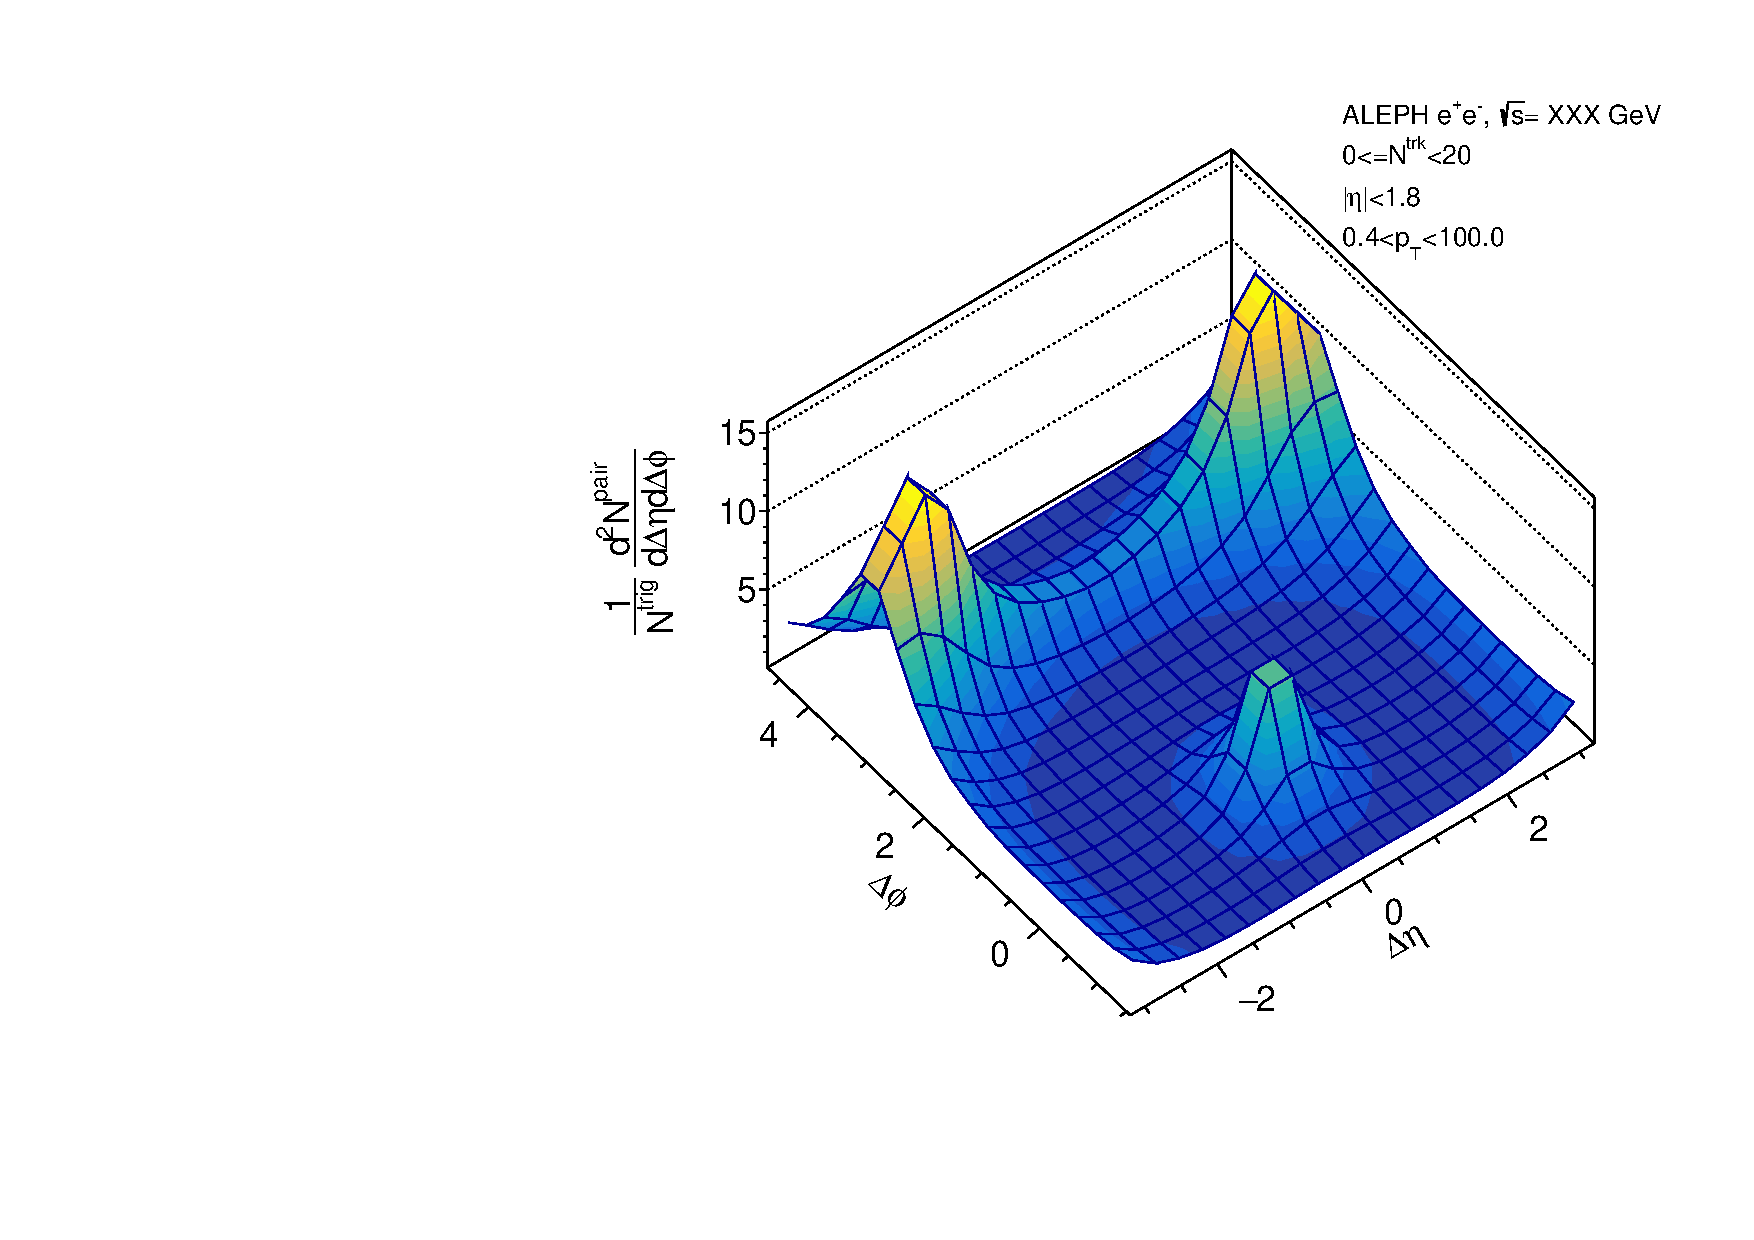
\includegraphics[width=.32\textwidth]{images/TwoParticleCorrelation/LEP1_BEAM/LEP1_BEAM_ratio1_0_20.pdf}}\hfill
\subfloat{\label{sfig:c}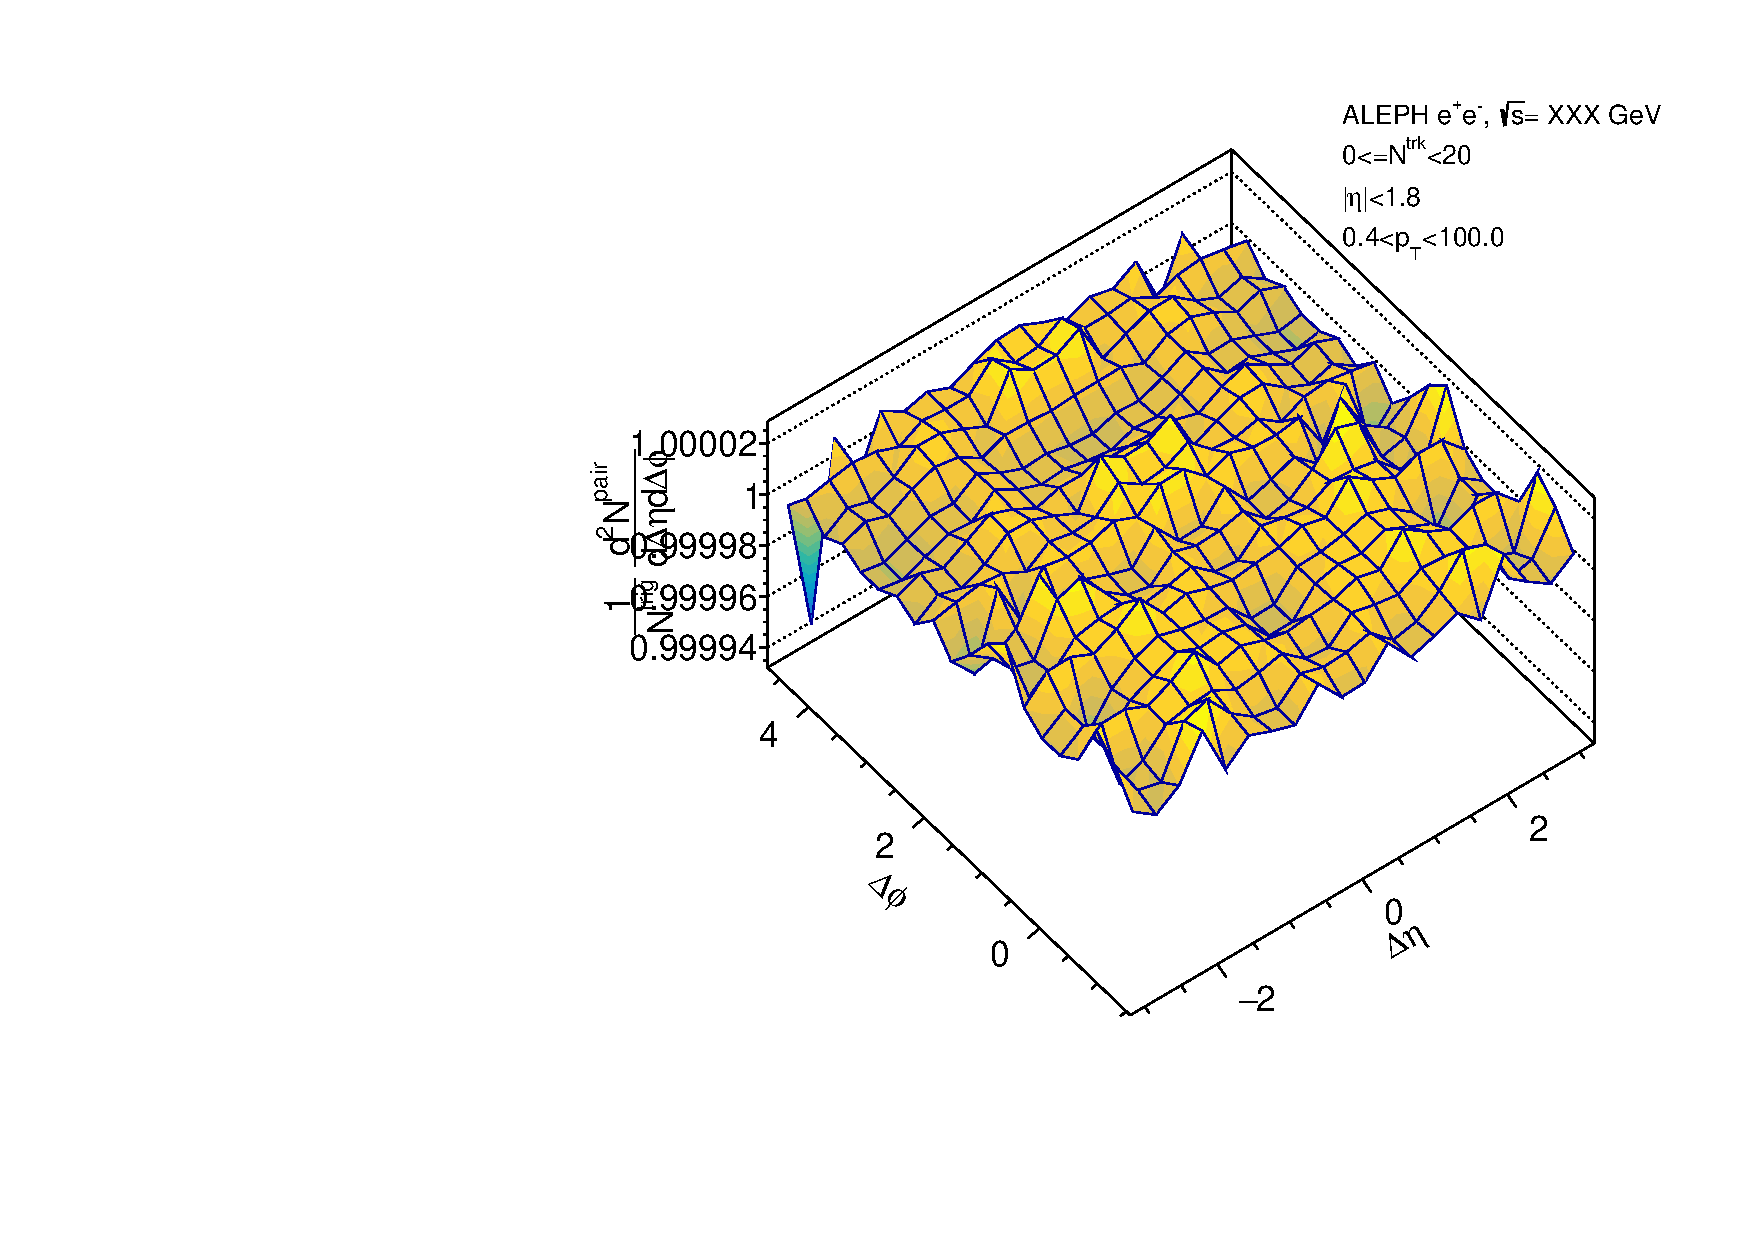
\includegraphics[width=.32\textwidth]{images/TwoParticleCorrelation/LEP1_BEAM/LEP1_BEAM_r_ratio_0_20.pdf}}\hfill
\subfloat{\label{sfig:d}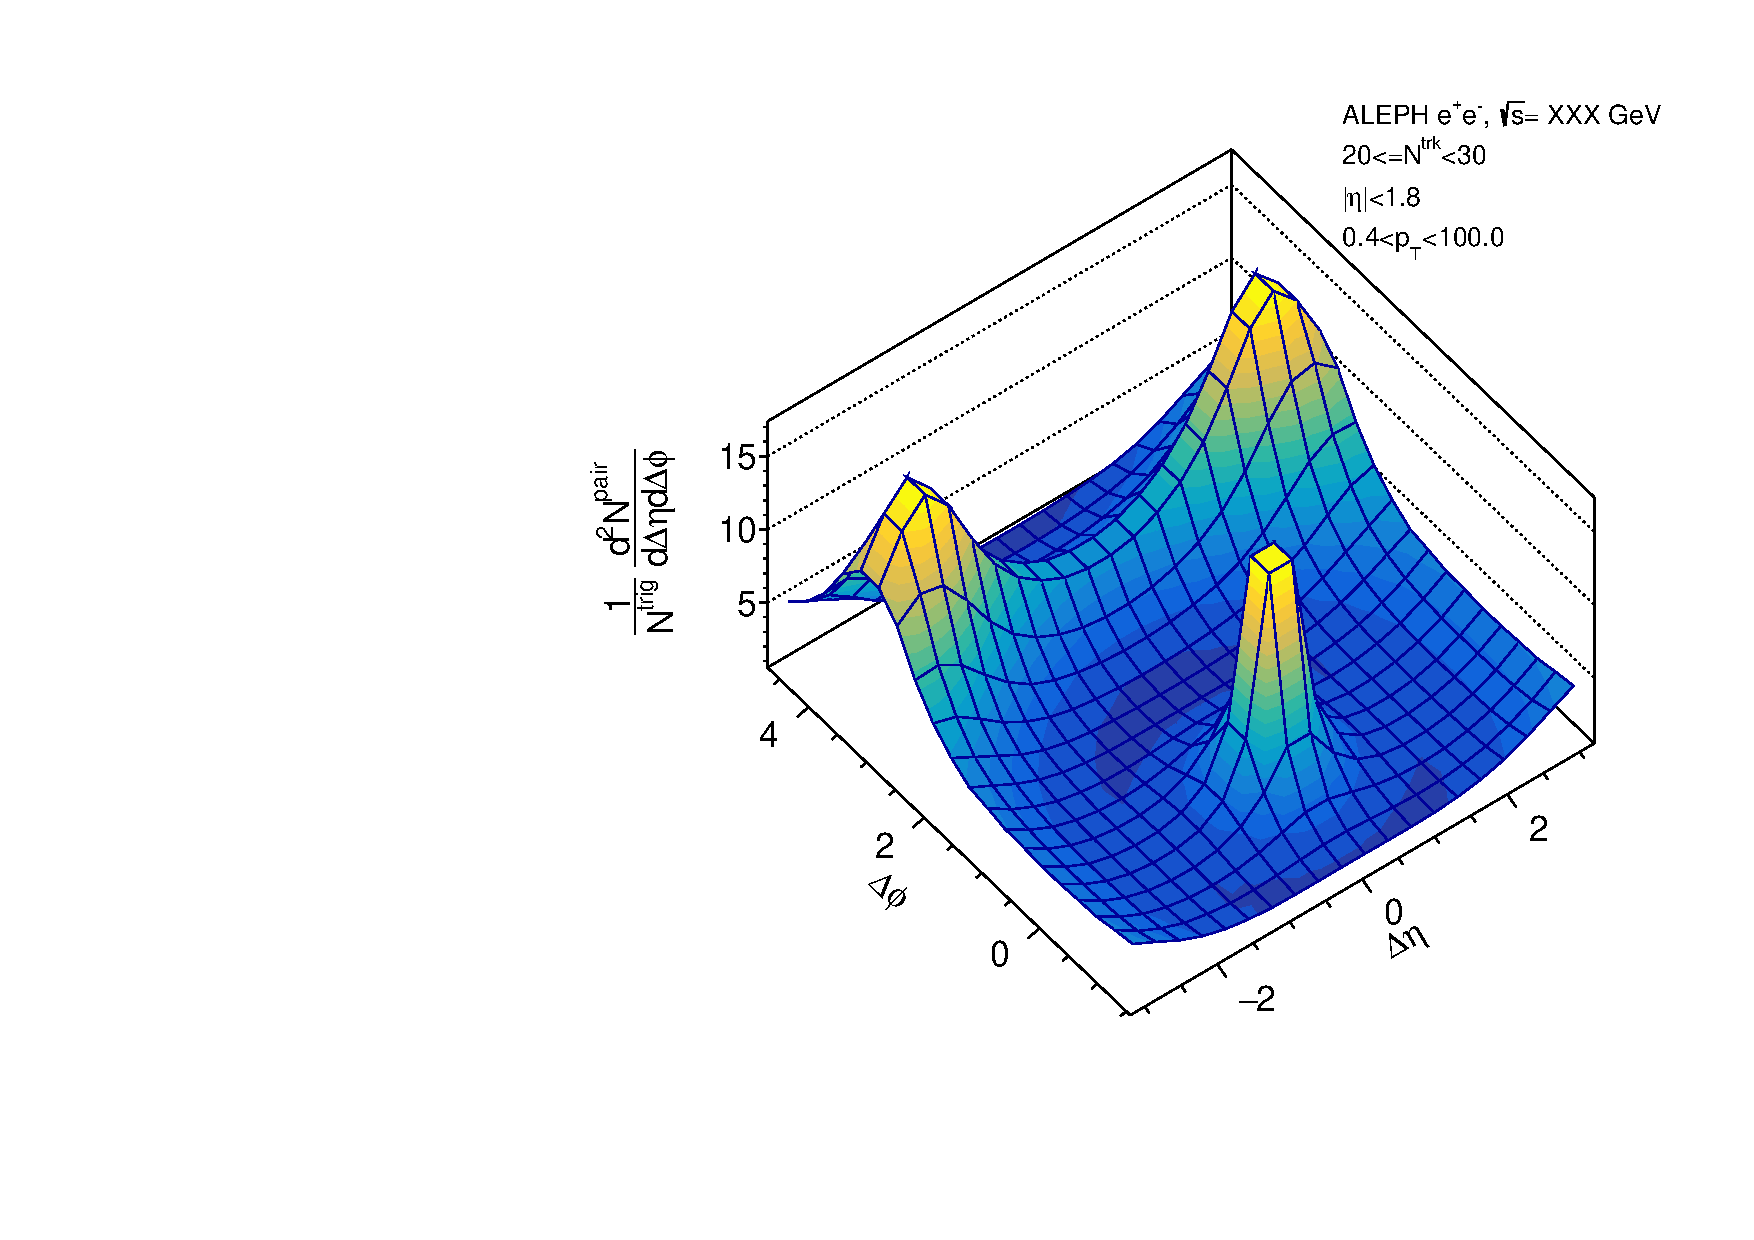
\includegraphics[width=.32\textwidth]{images/TwoParticleCorrelation/LEP1_BEAM/LEP1_BEAM_ratio2_20_30.pdf}}\hfill
\subfloat{\label{sfig:e}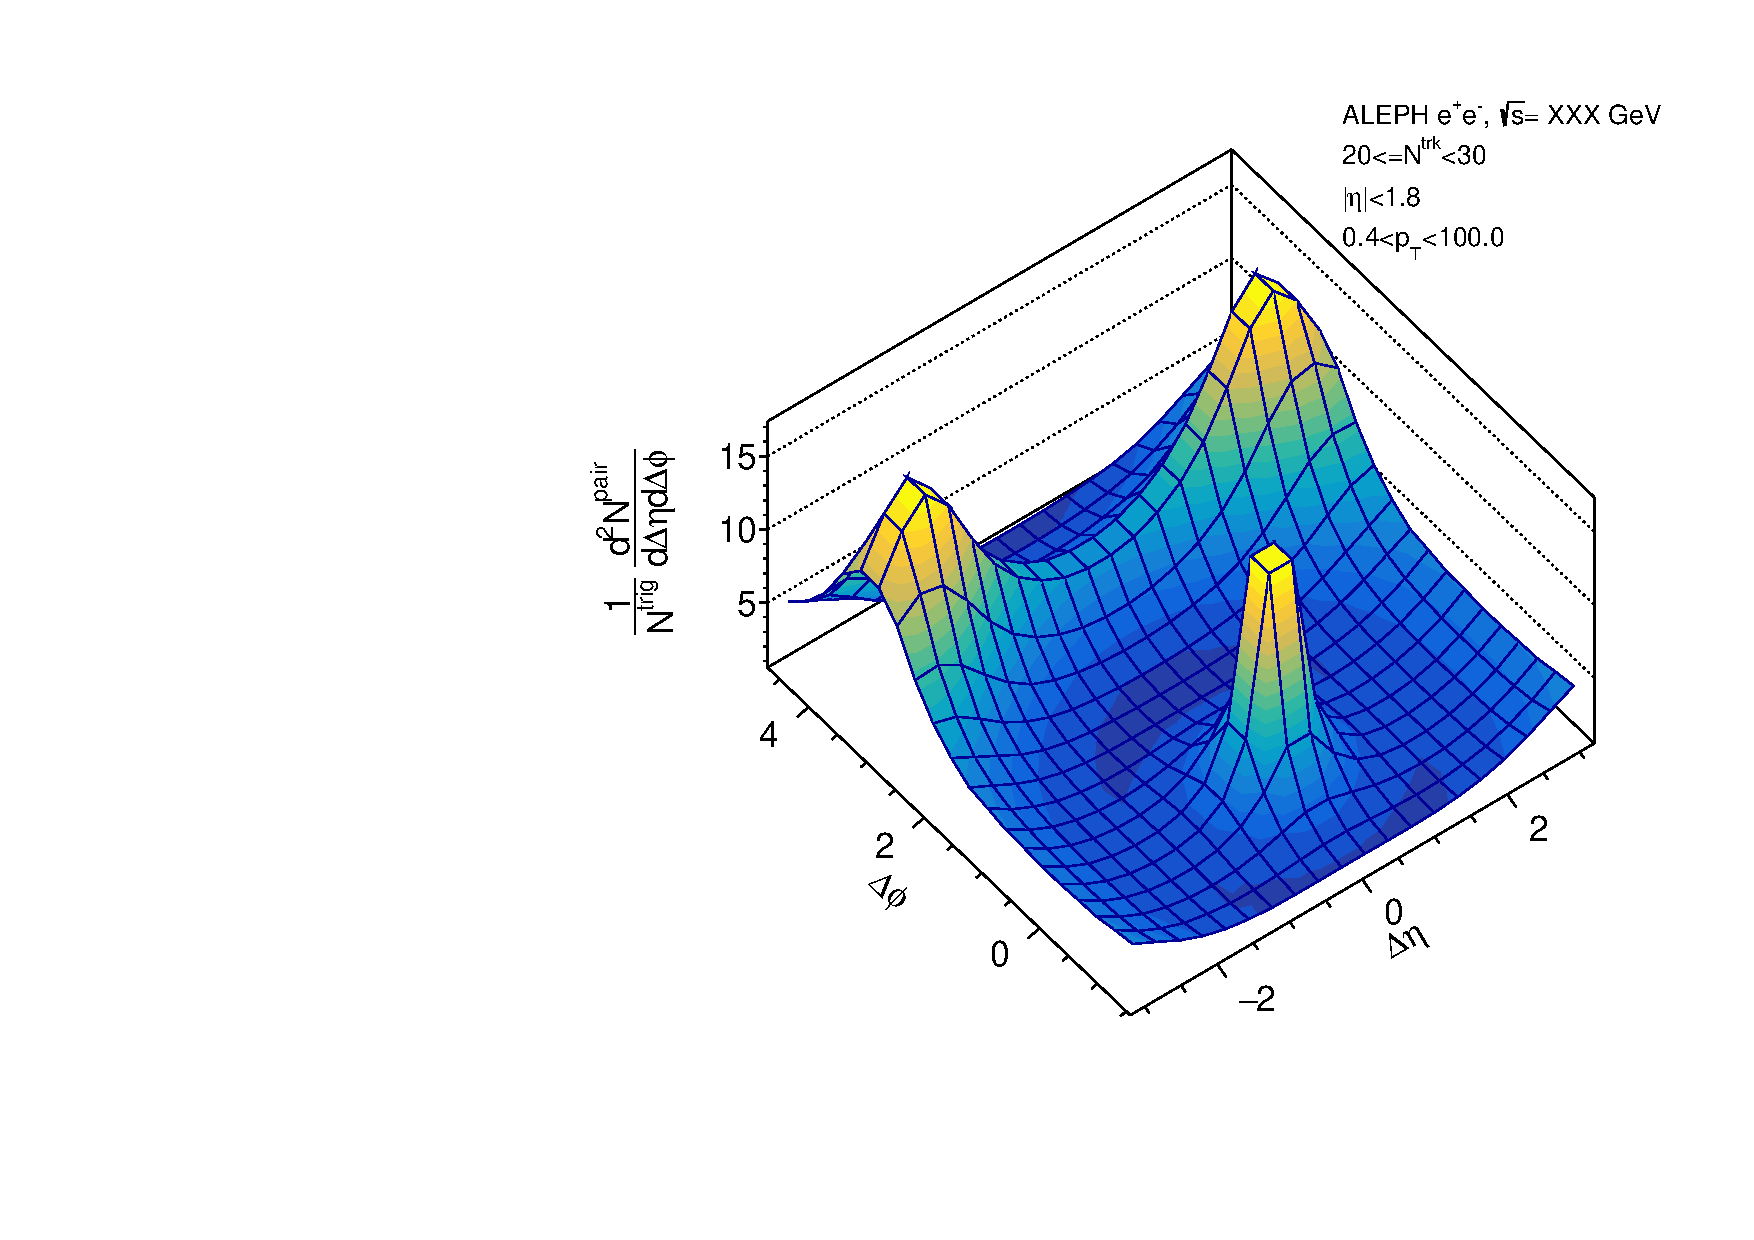
\includegraphics[width=.32\textwidth]{images/TwoParticleCorrelation/LEP1_BEAM/LEP1_BEAM_ratio1_20_30.pdf}}\hfill
\subfloat{\label{sfig:f}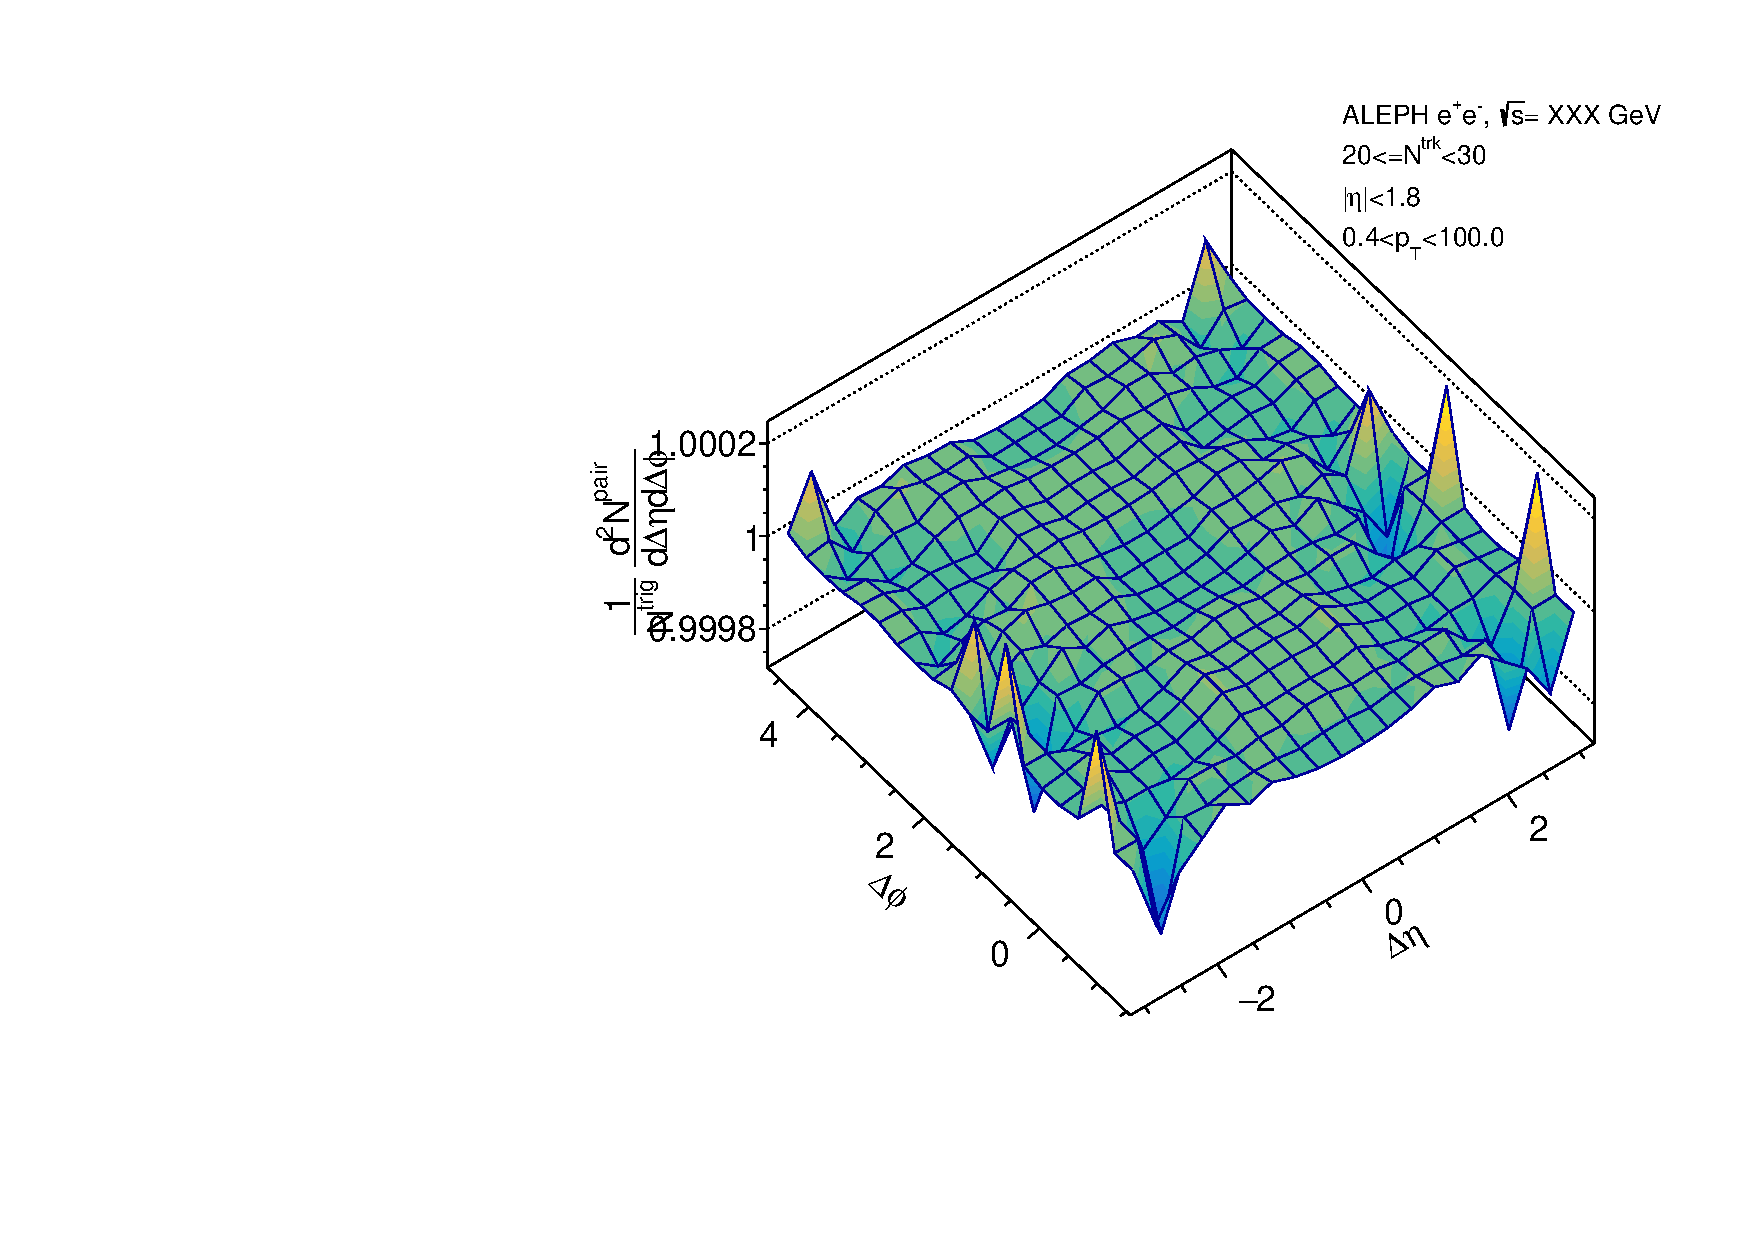
\includegraphics[width=.32\textwidth]{images/TwoParticleCorrelation/LEP1_BEAM/LEP1_BEAM_r_ratio_20_30.pdf}}\hfill
\subfloat{\label{sfig:g}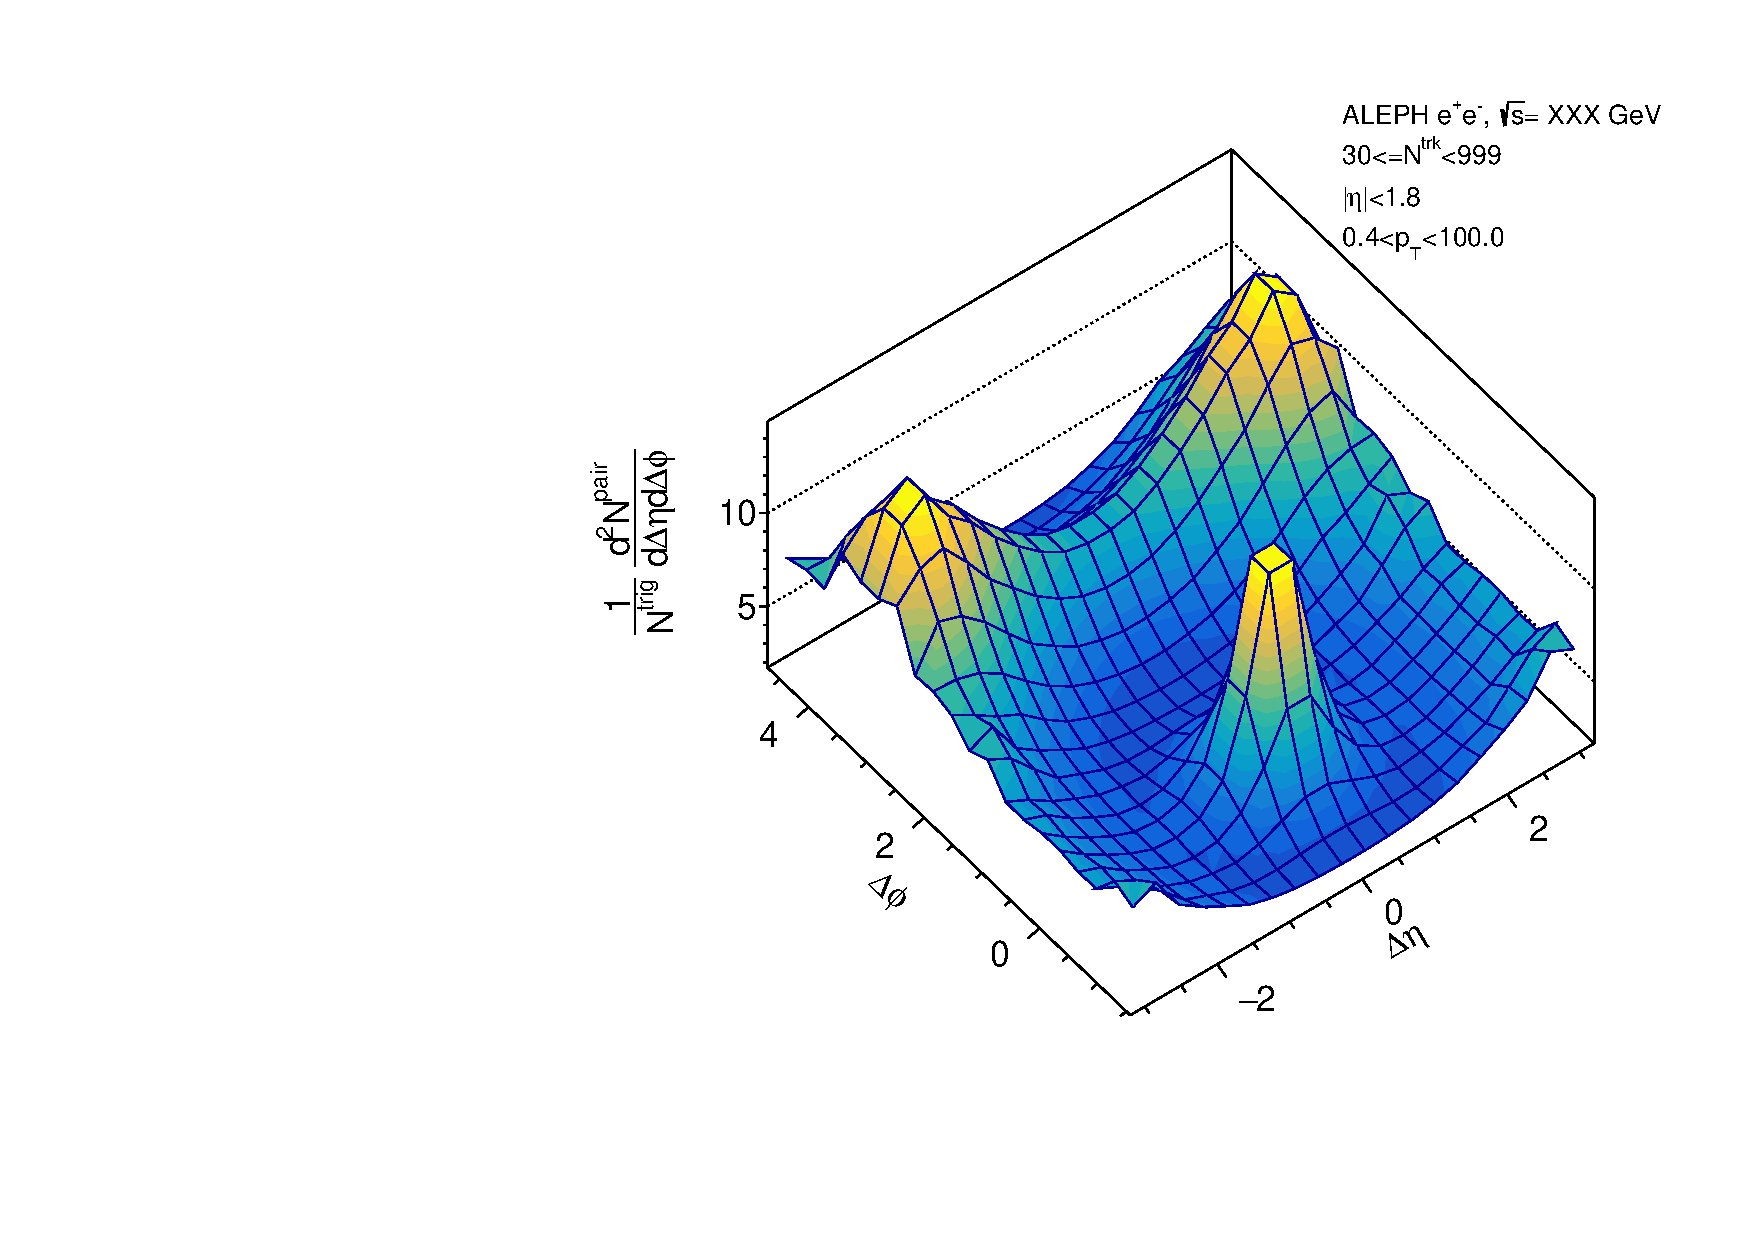
\includegraphics[width=.32\textwidth]{images/TwoParticleCorrelation/LEP1_BEAM/LEP1_BEAM_ratio2_30_999.pdf}}\hfill
\subfloat{\label{sfig:h}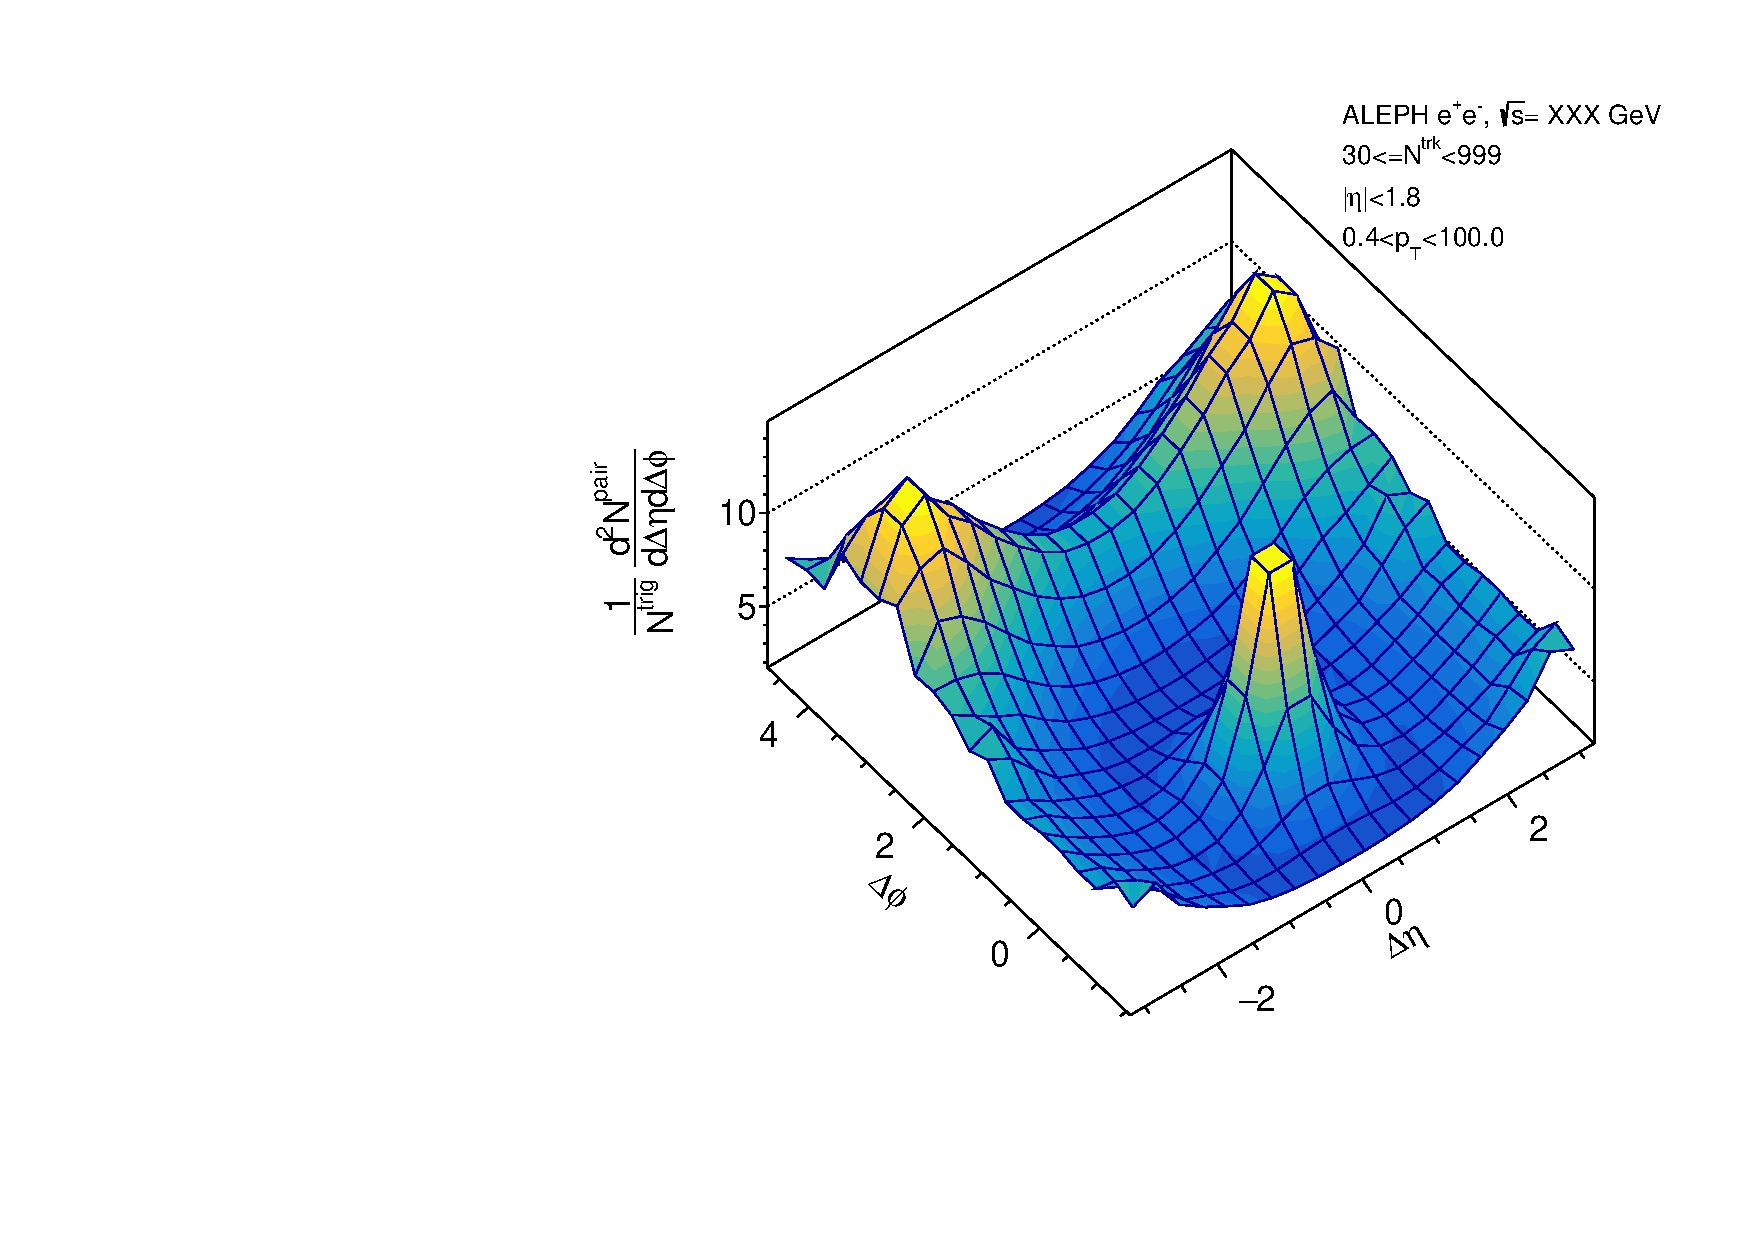
\includegraphics[width=.32\textwidth]{images/TwoParticleCorrelation/LEP1_BEAM/LEP1_BEAM_ratio1_30_999.pdf}}\hfill
\subfloat{\label{sfig:i}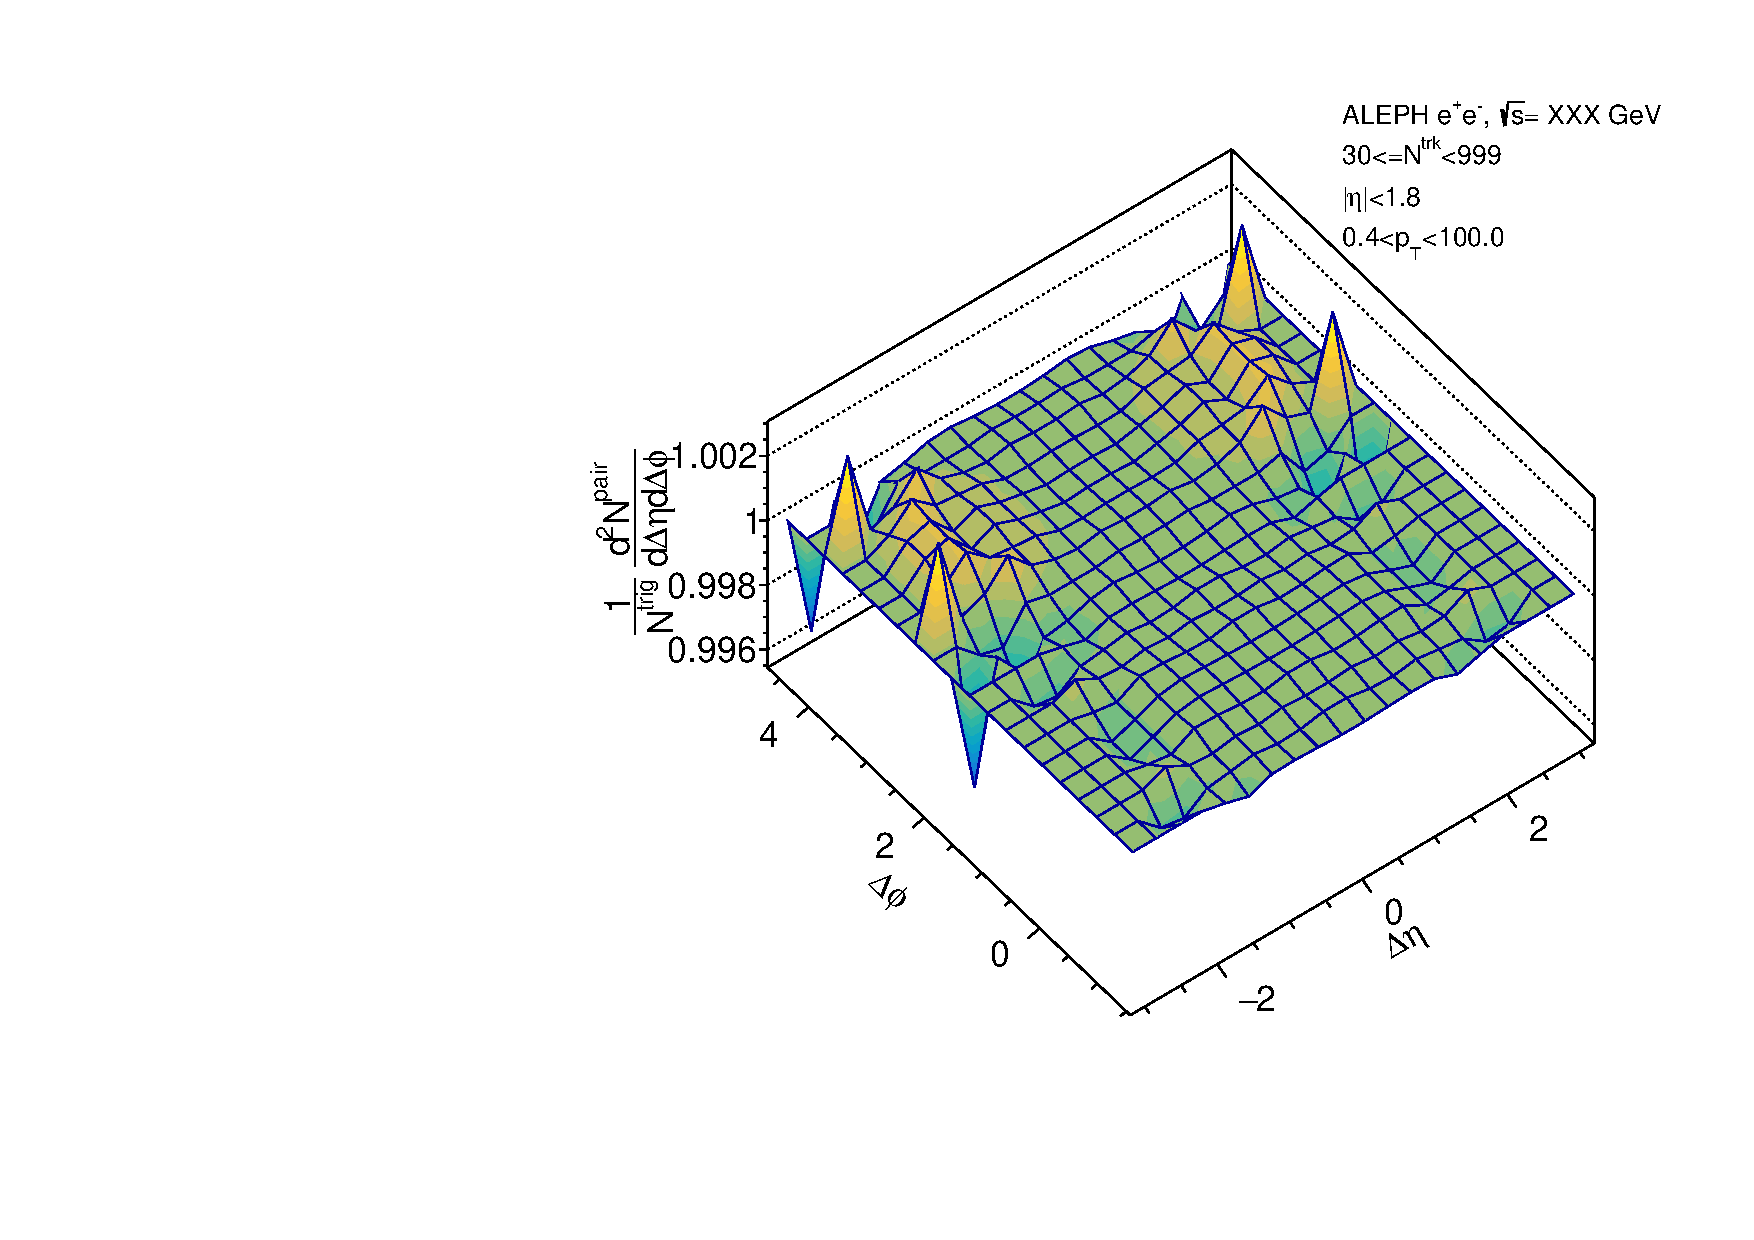
\includegraphics[width=.32\textwidth]{images/TwoParticleCorrelation/LEP1_BEAM/LEP1_BEAM_r_ratio_30_999.pdf}} \\
\caption{Two particle correlation fuctions for the LEP1 data set analyzed in the beam axis.}
\label{fig:test}
\end{figure}

\begin{figure}[h!]
\centering
\subfloat{\label{sfig:a}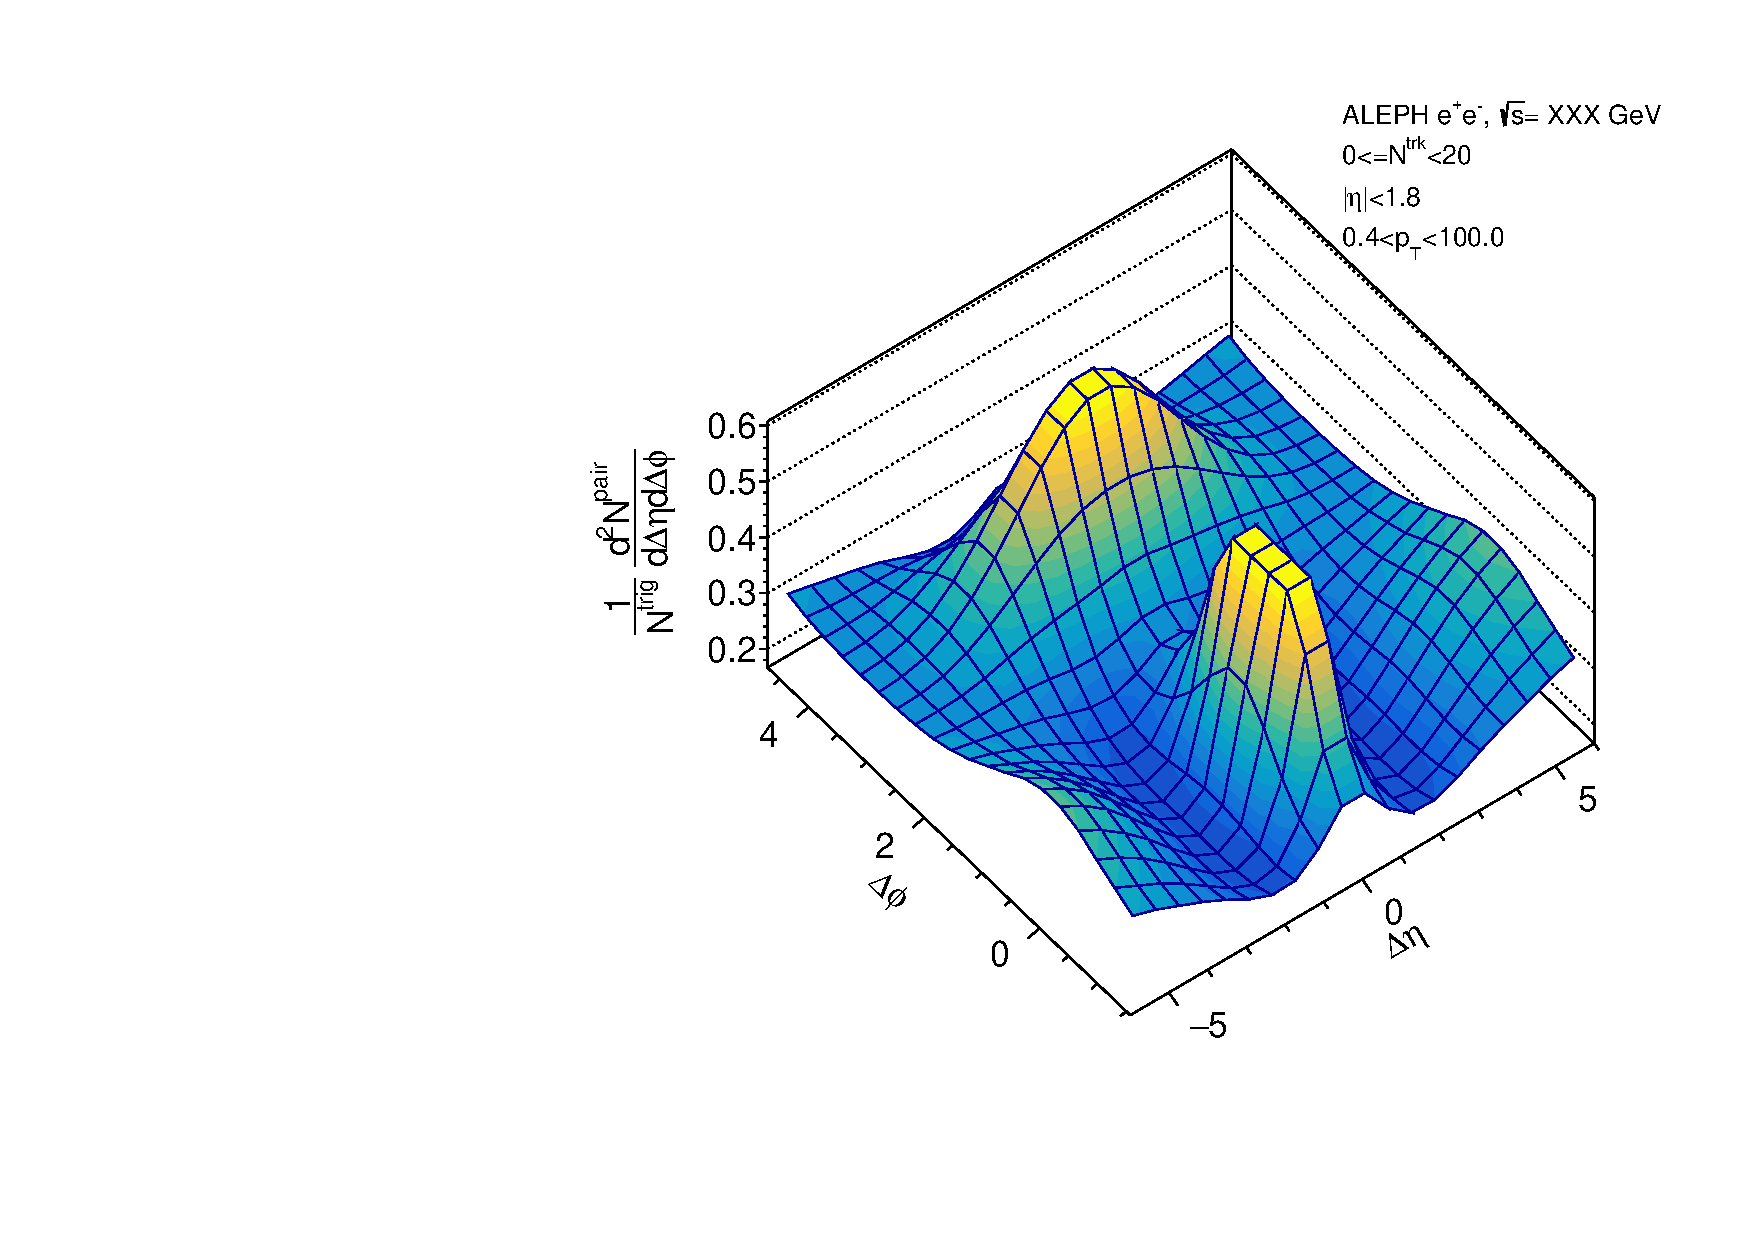
\includegraphics[width=.32\textwidth]{images/TwoParticleCorrelation/LEP1_THRUST/LEP1_THRUST_ratio2_0_20.pdf}}\hfill
\subfloat{\label{sfig:b}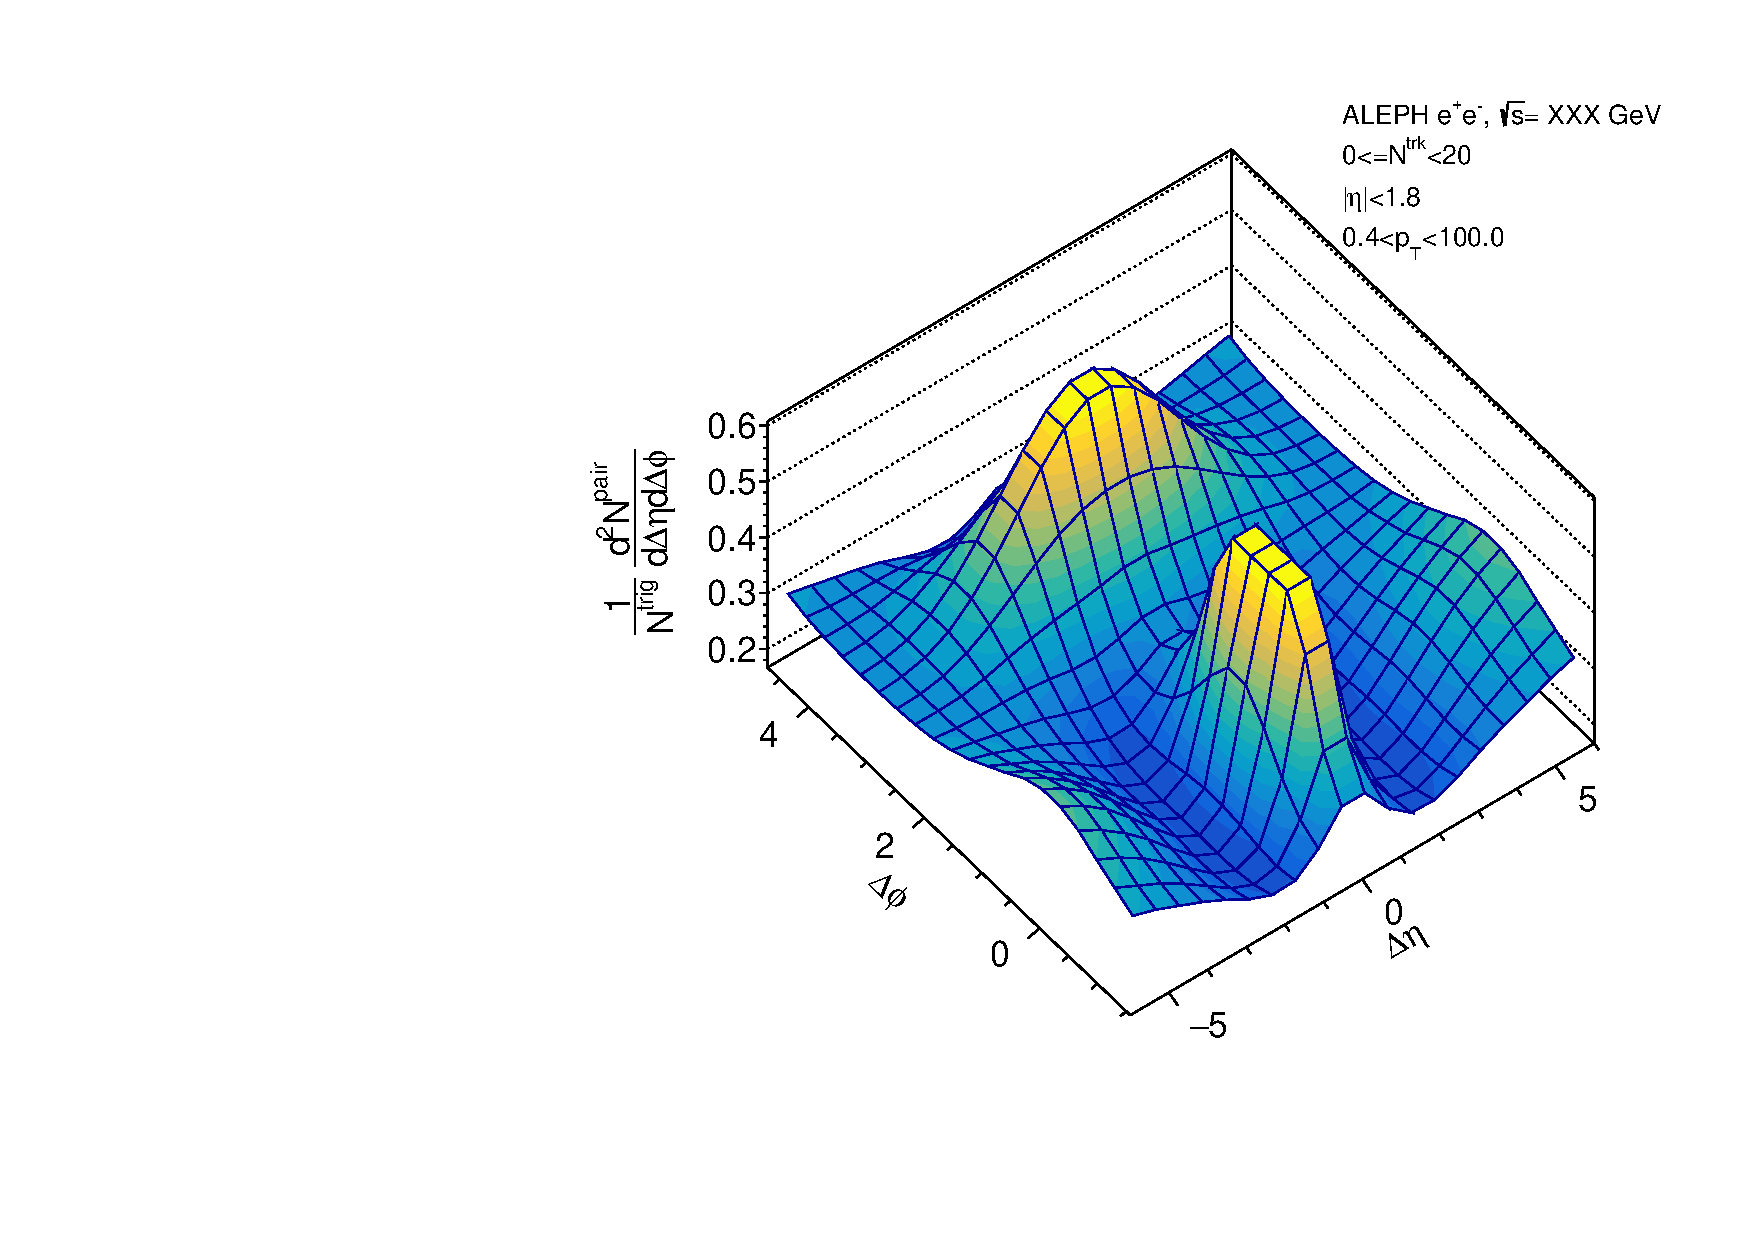
\includegraphics[width=.32\textwidth]{images/TwoParticleCorrelation/LEP1_THRUST/LEP1_THRUST_ratio1_0_20.pdf}}\hfill
\subfloat{\label{sfig:c}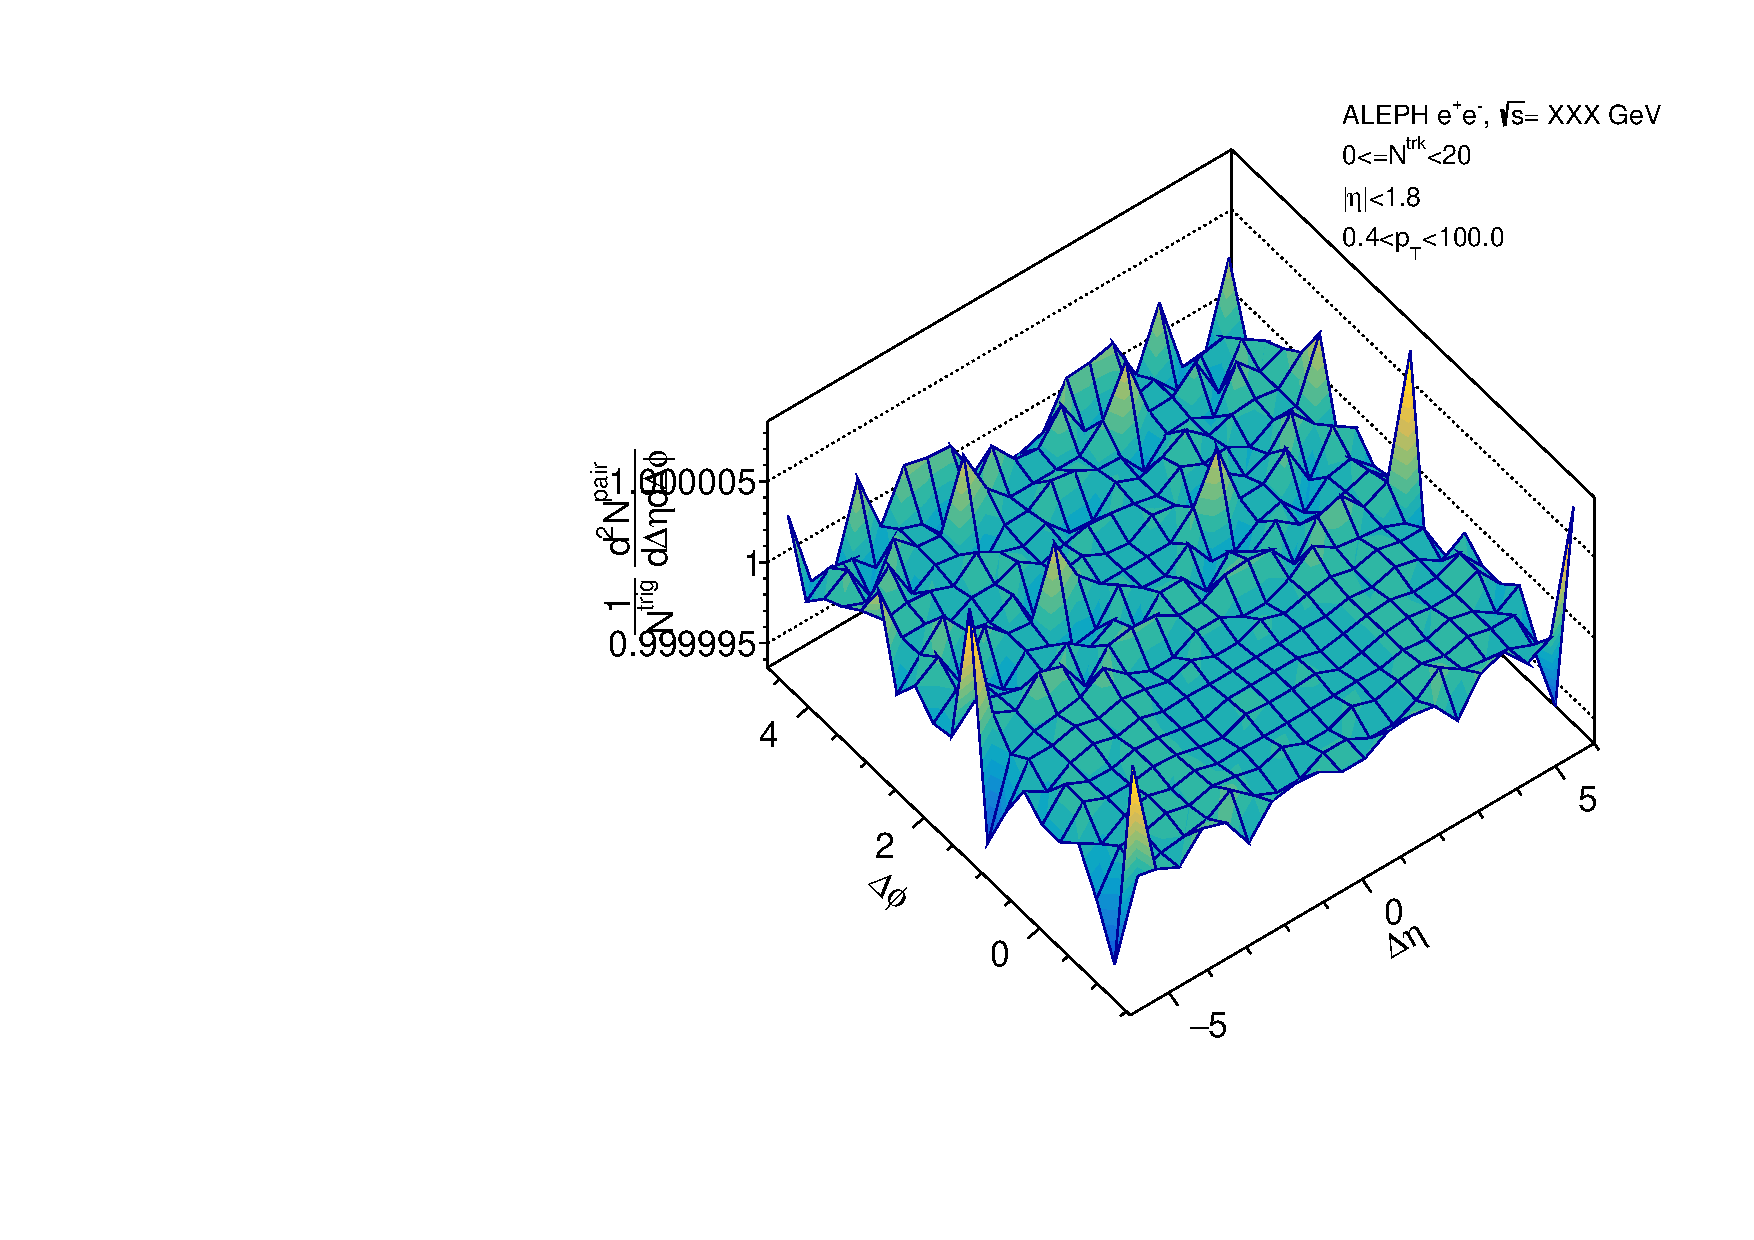
\includegraphics[width=.32\textwidth]{images/TwoParticleCorrelation/LEP1_THRUST/LEP1_THRUST_r_ratio_0_20.pdf}}\hfill
\subfloat{\label{sfig:d}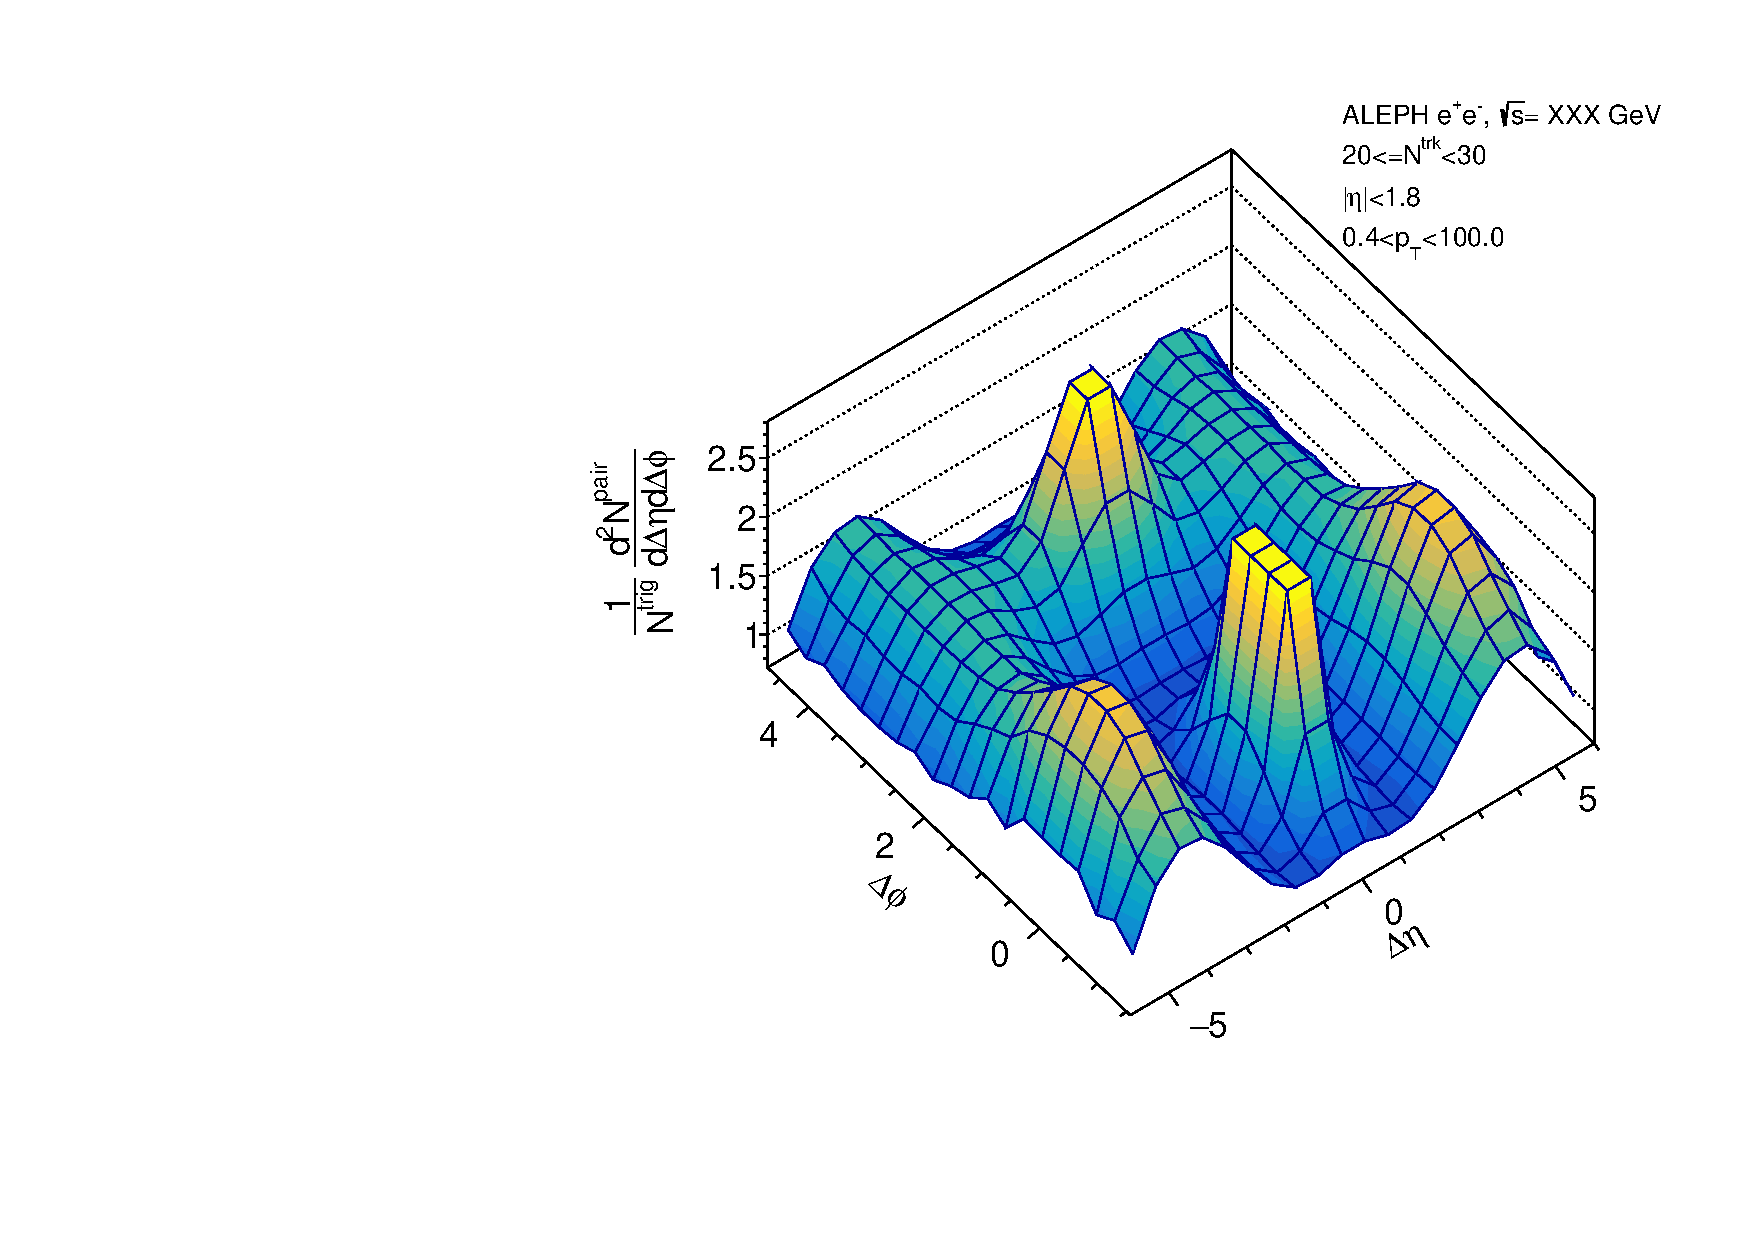
\includegraphics[width=.32\textwidth]{images/TwoParticleCorrelation/LEP1_THRUST/LEP1_THRUST_ratio2_20_30.pdf}}\hfill
\subfloat{\label{sfig:e}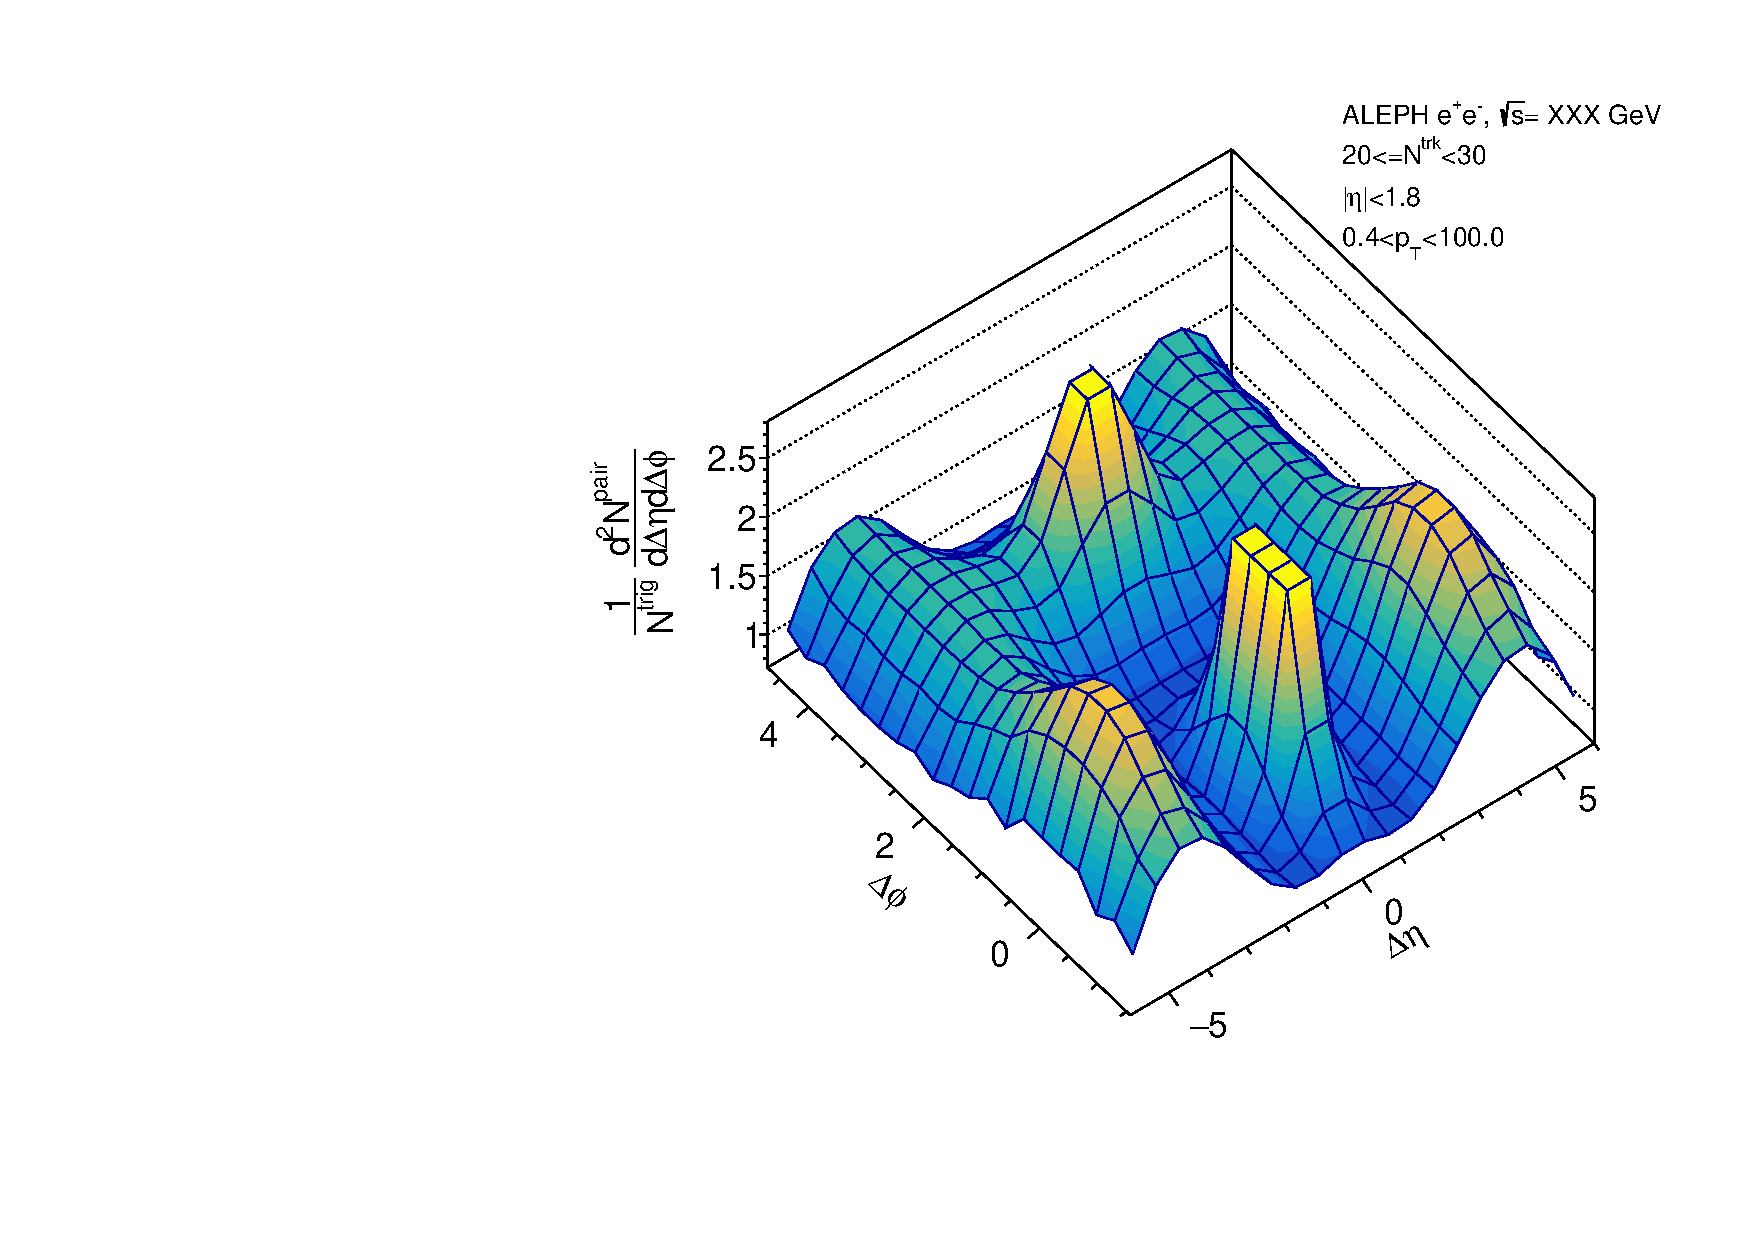
\includegraphics[width=.32\textwidth]{images/TwoParticleCorrelation/LEP1_THRUST/LEP1_THRUST_ratio1_20_30.pdf}}\hfill
\subfloat{\label{sfig:f}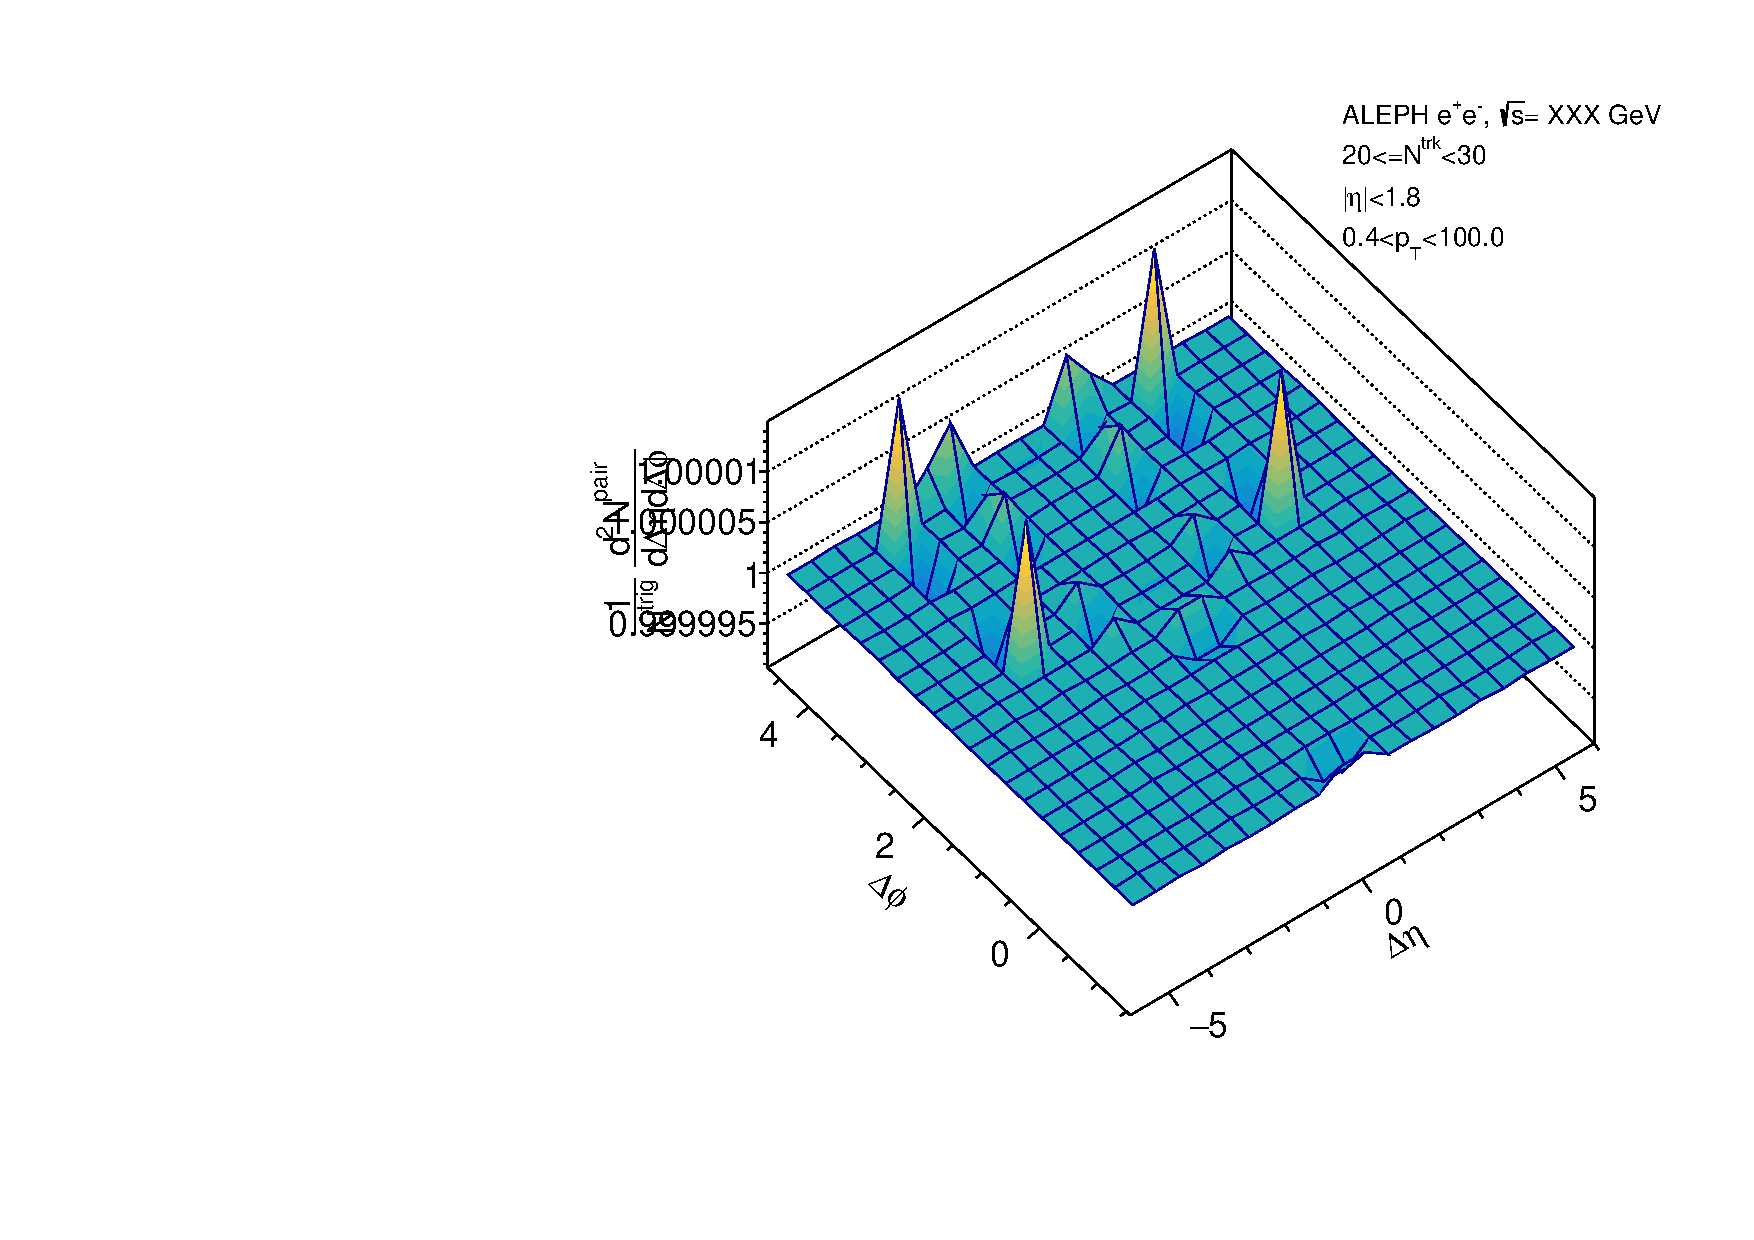
\includegraphics[width=.32\textwidth]{images/TwoParticleCorrelation/LEP1_THRUST/LEP1_THRUST_r_ratio_20_30.pdf}}\hfill
\subfloat{\label{sfig:g}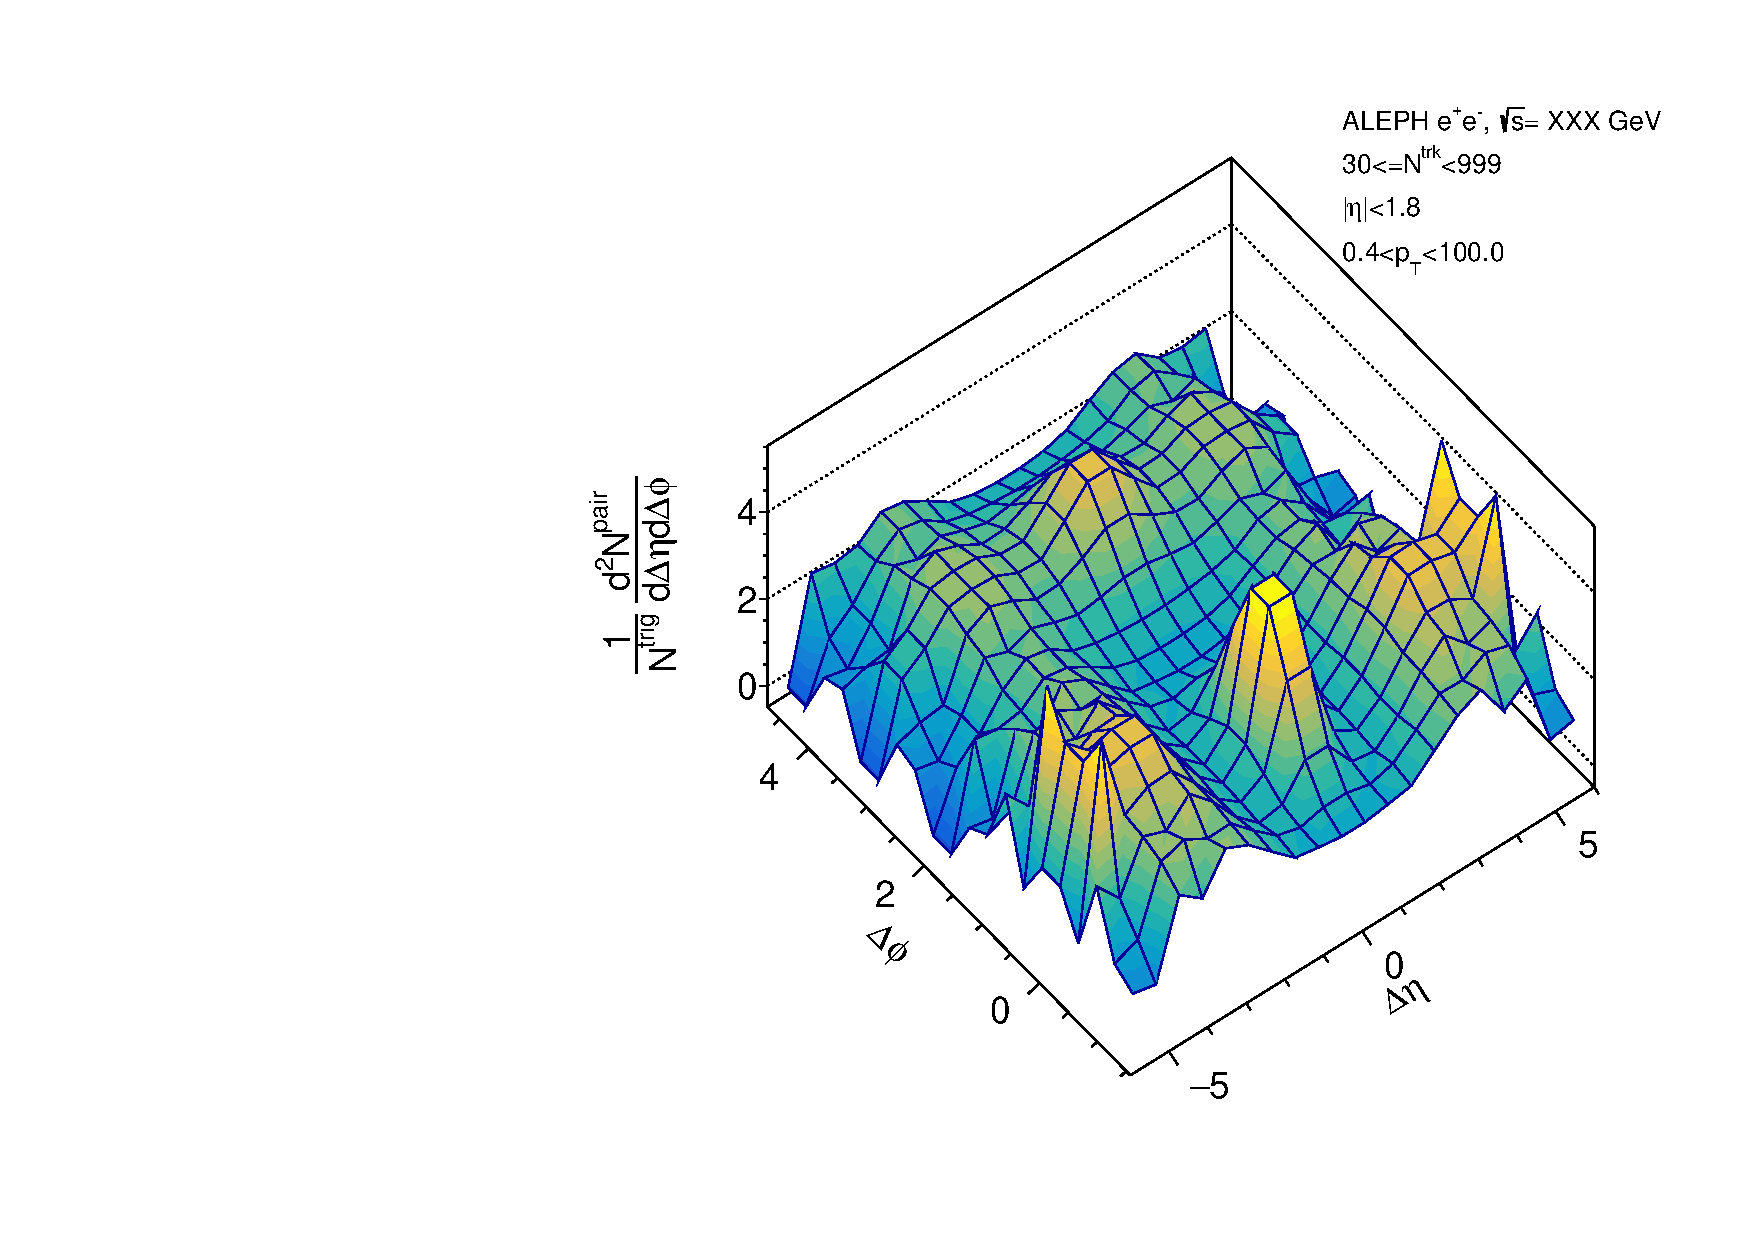
\includegraphics[width=.32\textwidth]{images/TwoParticleCorrelation/LEP1_THRUST/LEP1_THRUST_ratio2_30_999.pdf}}\hfill
\subfloat{\label{sfig:h}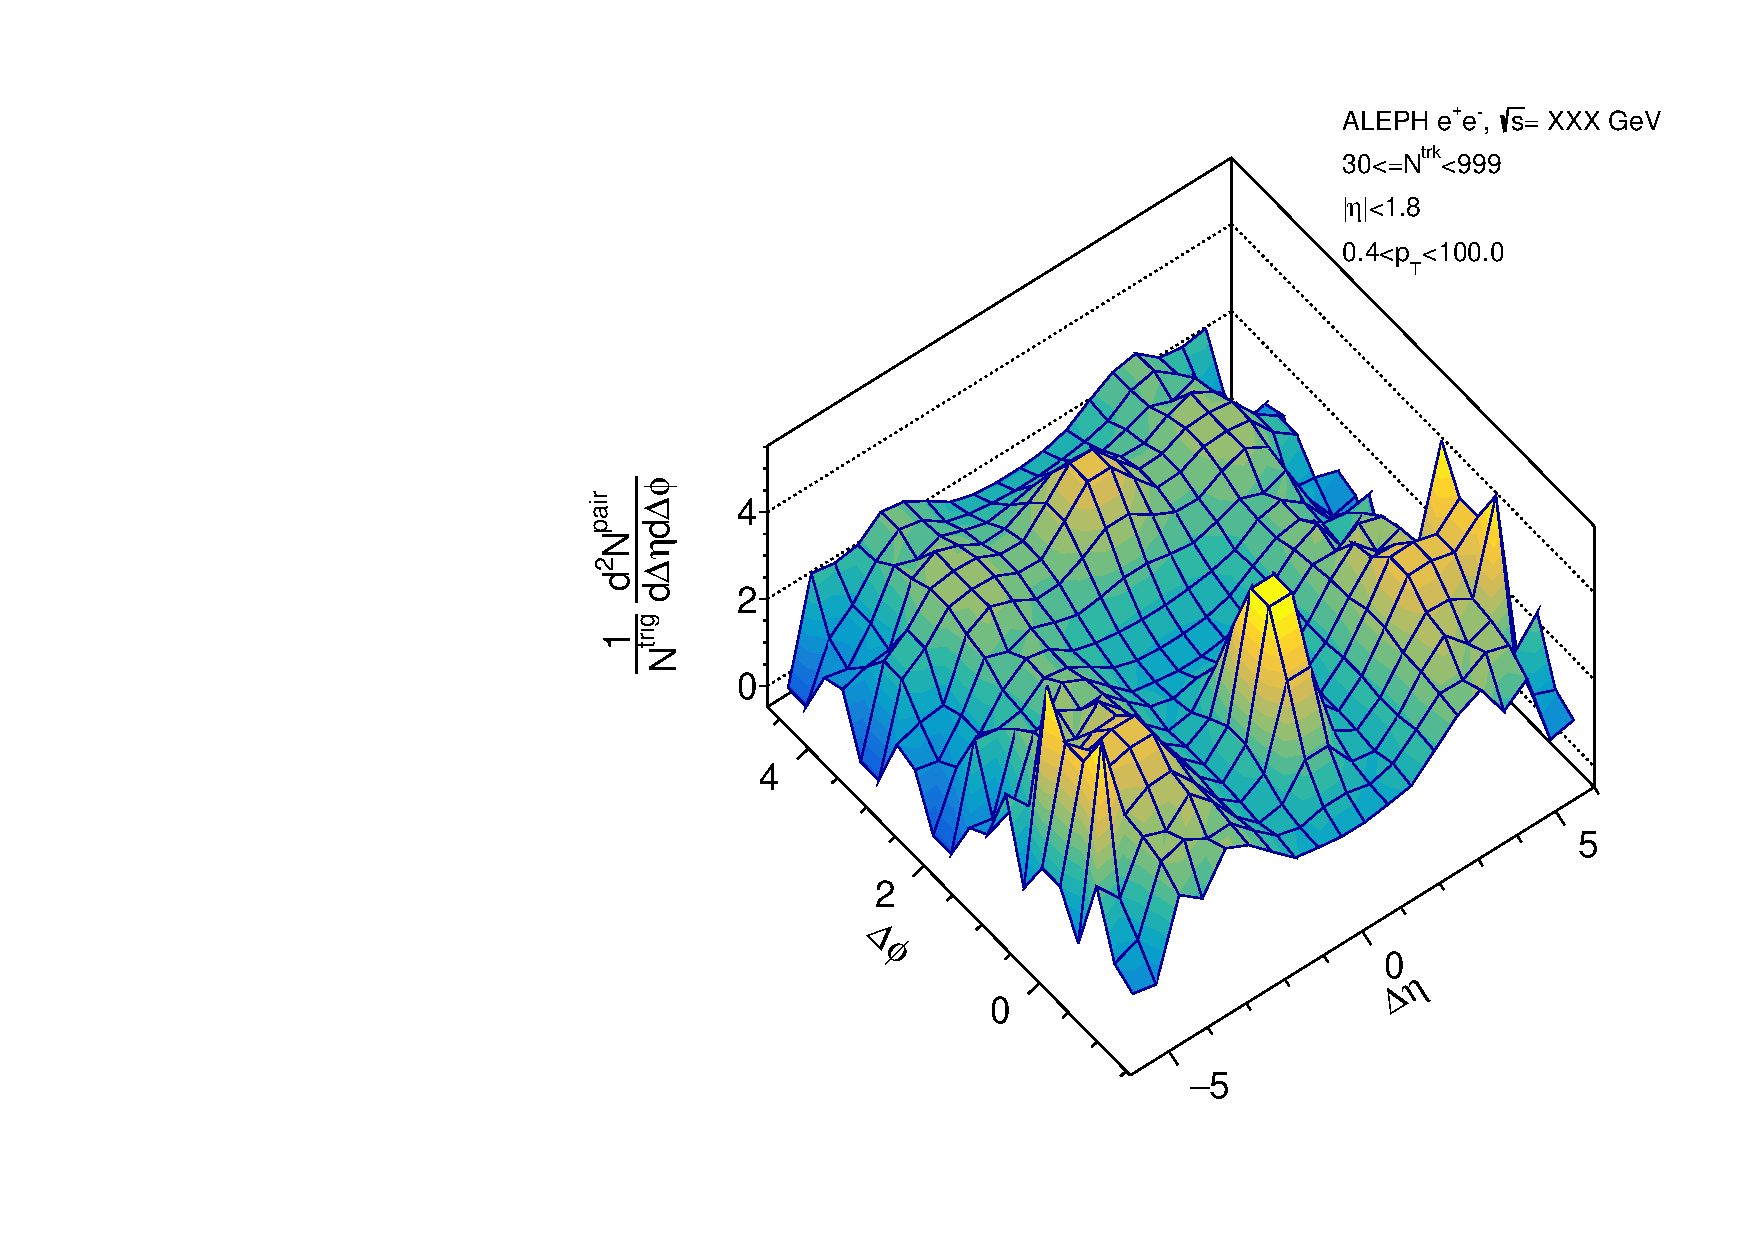
\includegraphics[width=.32\textwidth]{images/TwoParticleCorrelation/LEP1_THRUST/LEP1_THRUST_ratio1_30_999.pdf}}\hfill
\subfloat{\label{sfig:i}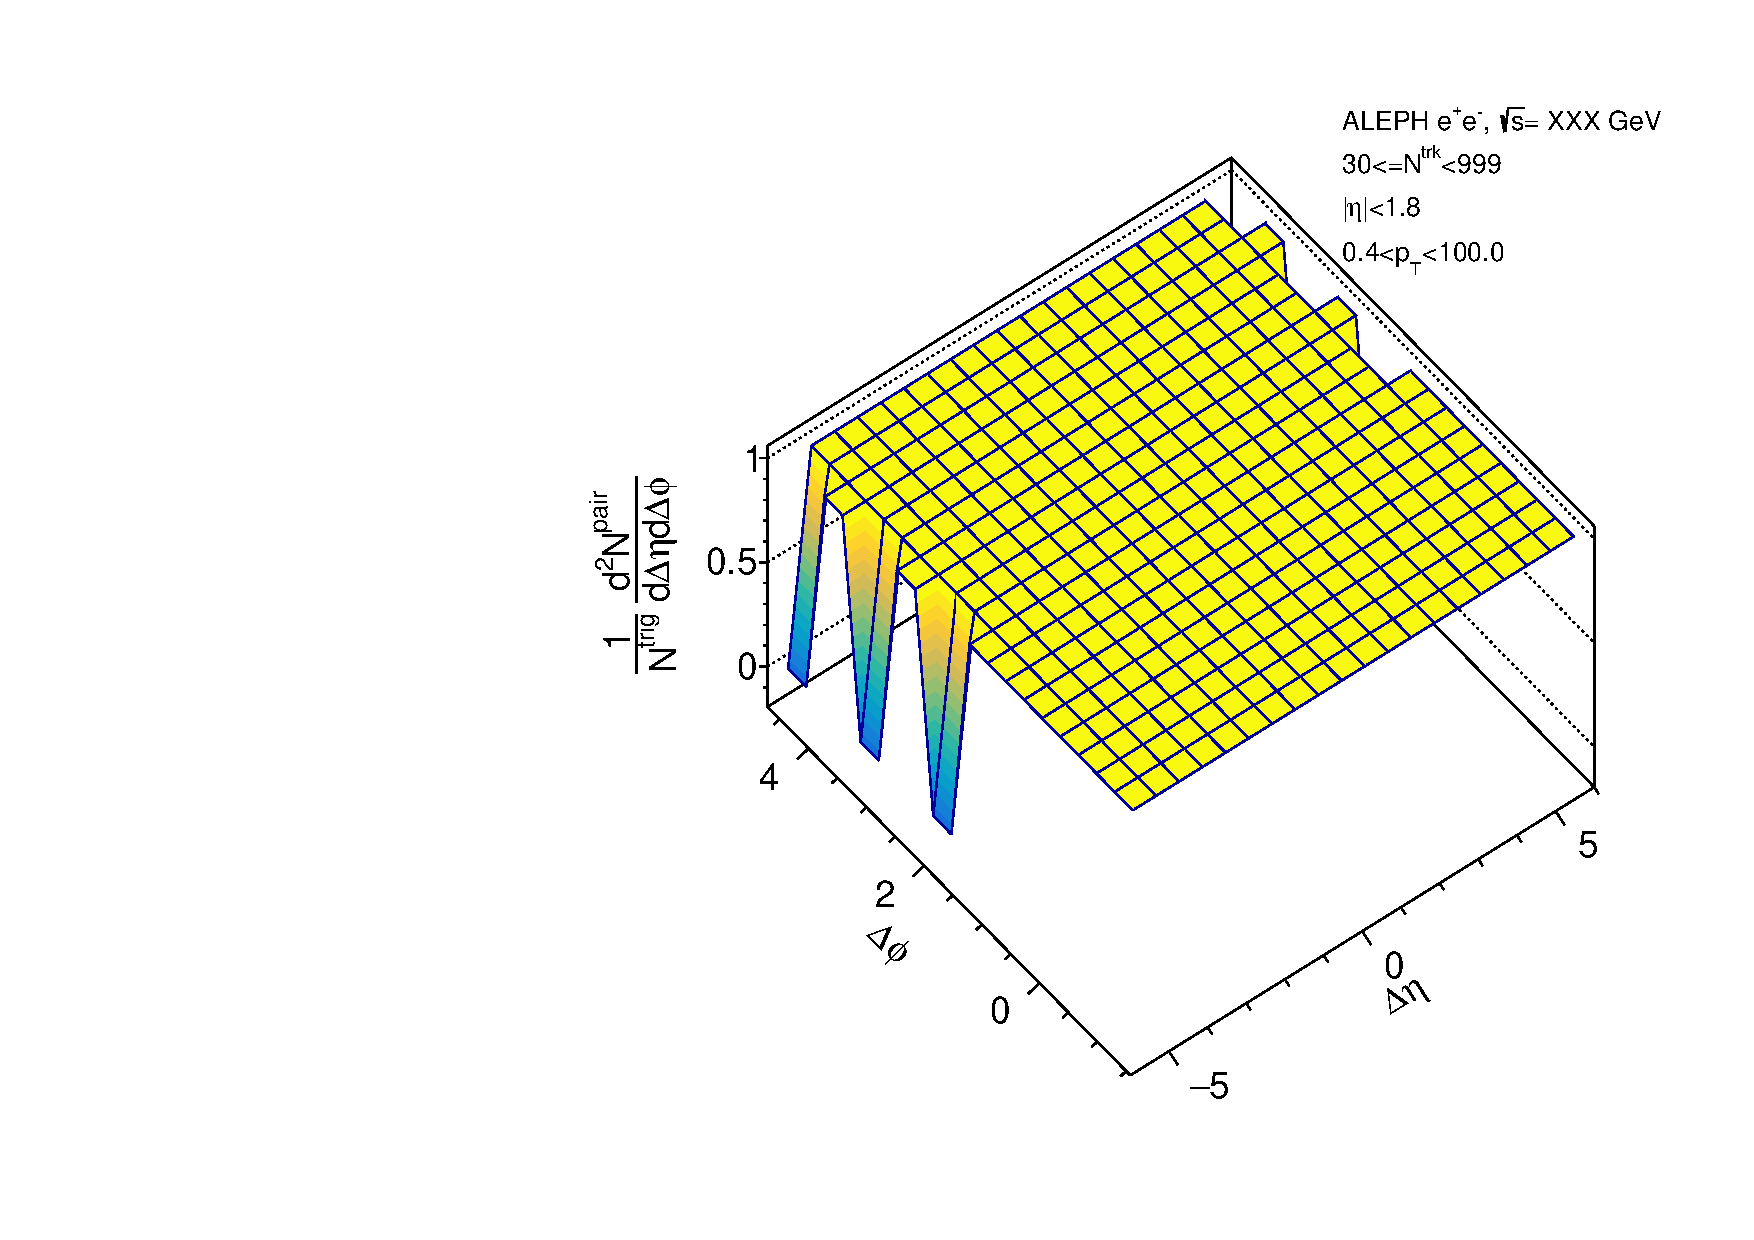
\includegraphics[width=.32\textwidth]{images/TwoParticleCorrelation/LEP1_THRUST/LEP1_THRUST_r_ratio_30_999.pdf}} \\
\caption{Two particle correlation fuctions for the LEP1 data set analyzed in the thrust axis.}
\label{fig:test}
\end{figure}

\begin{figure}[h!]
\centering
\subfloat{\label{sfig:a}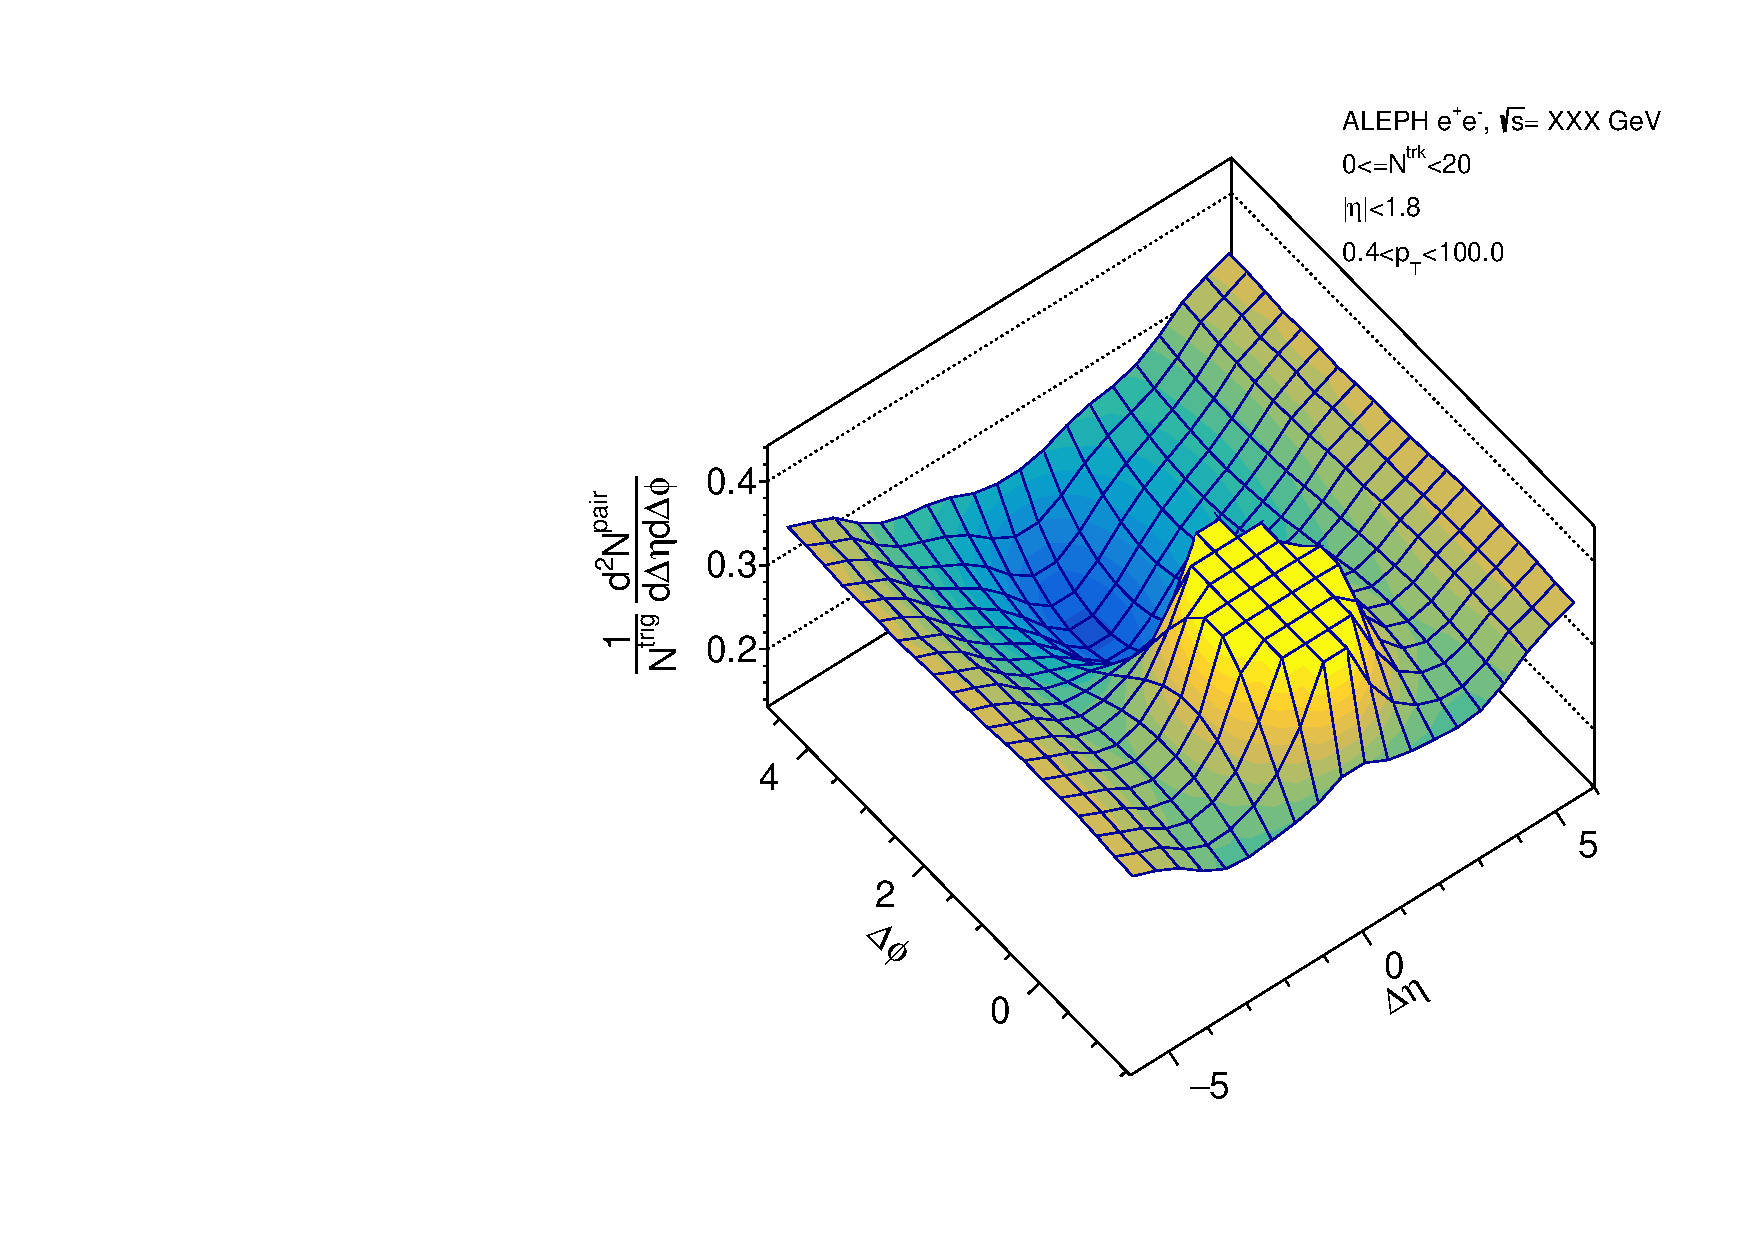
\includegraphics[width=.32\textwidth]{images/TwoParticleCorrelation/LEP1_WTA/LEP1_WTA_ratio2_0_20.pdf}}\hfill
\subfloat{\label{sfig:b}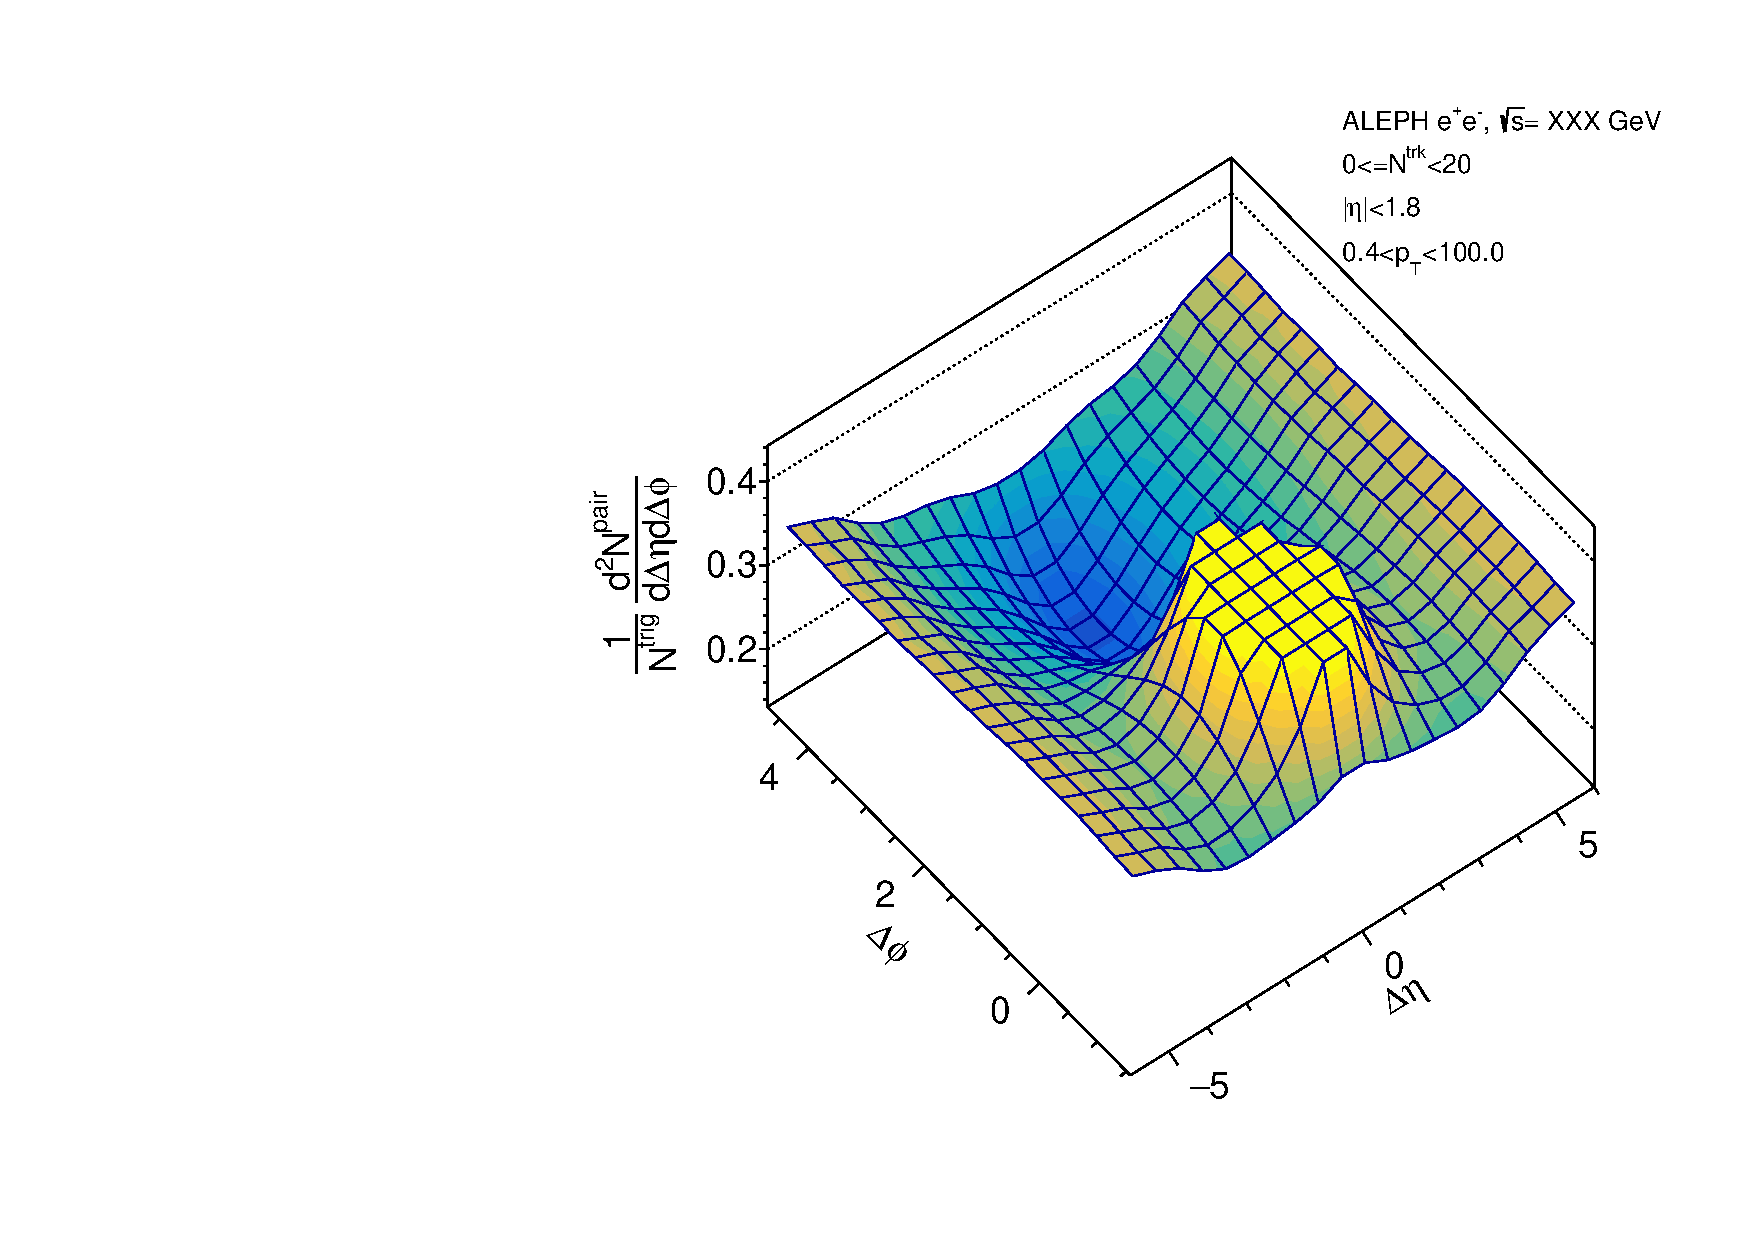
\includegraphics[width=.32\textwidth]{images/TwoParticleCorrelation/LEP1_WTA/LEP1_WTA_ratio1_0_20.pdf}}\hfill
\subfloat{\label{sfig:c}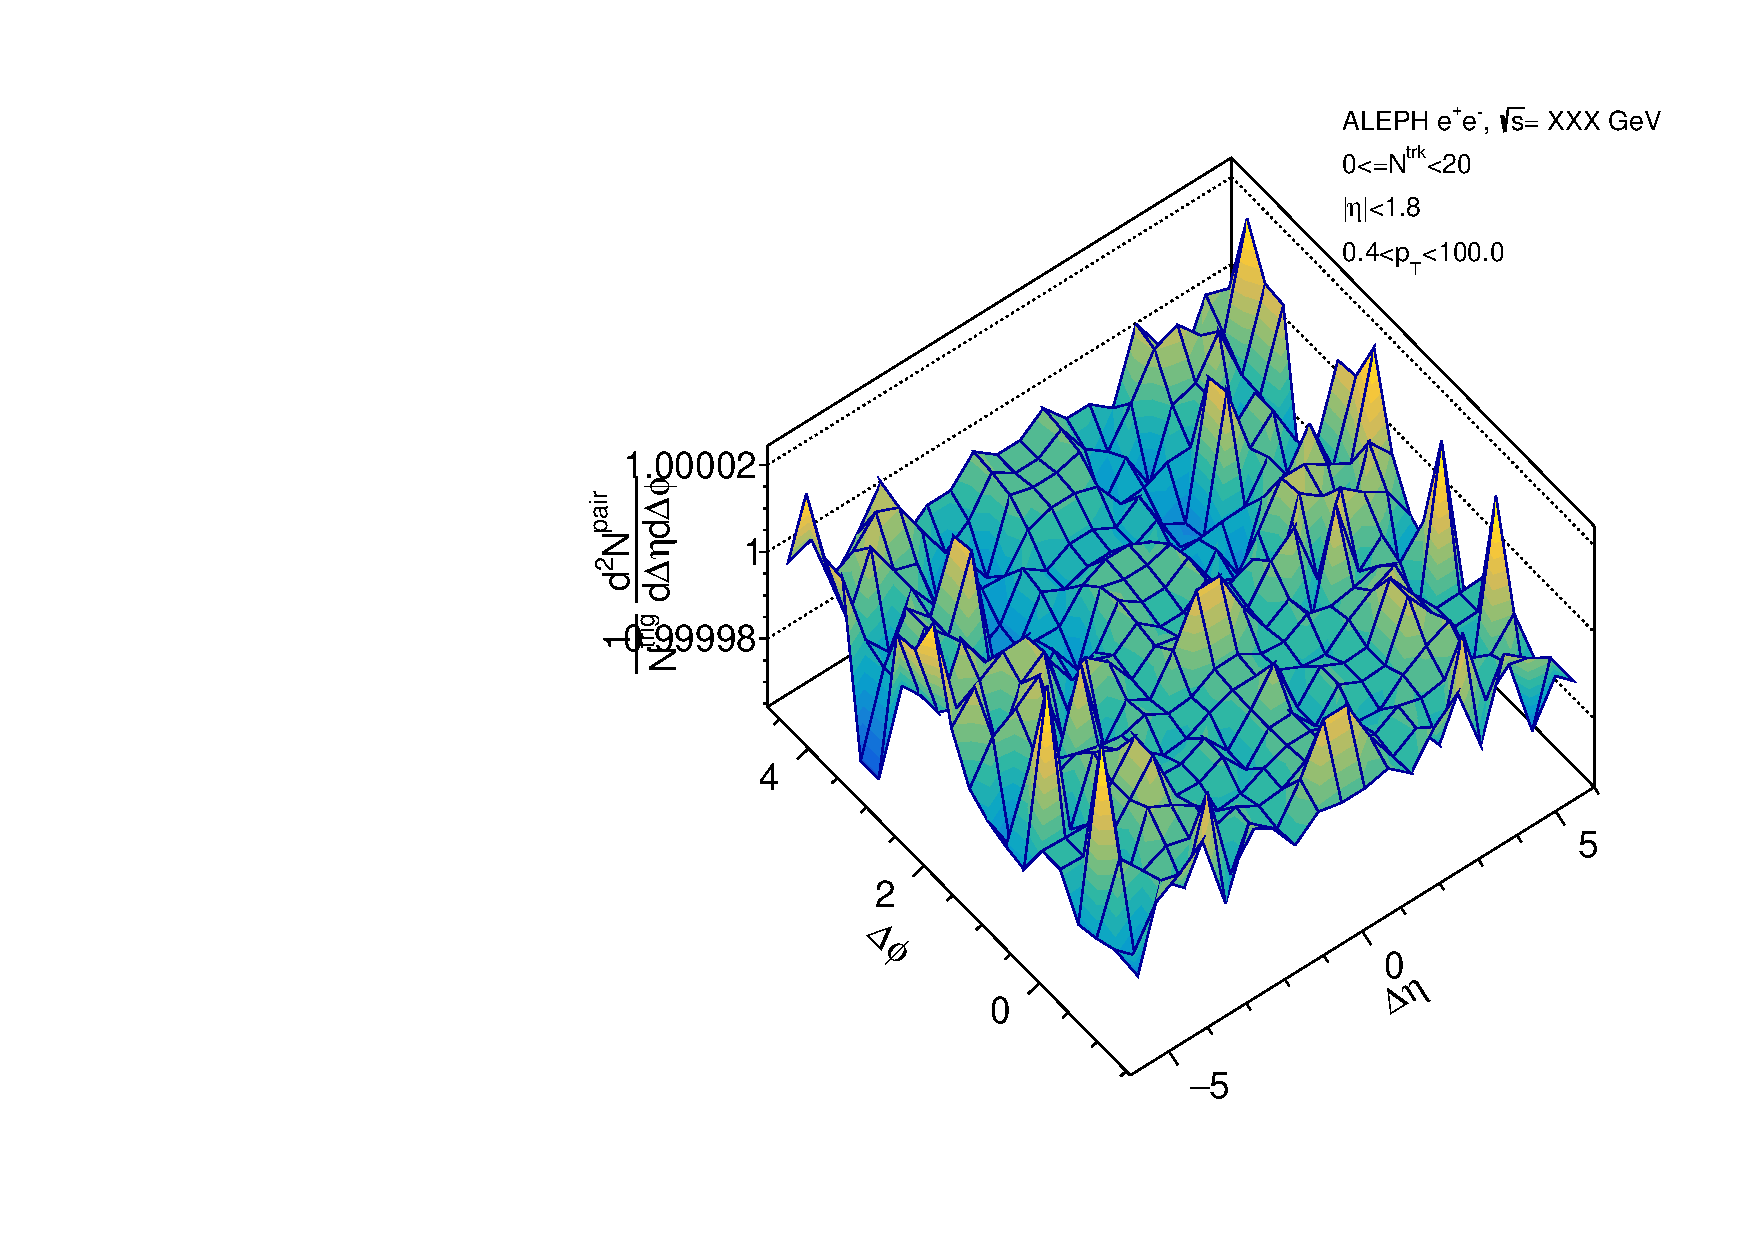
\includegraphics[width=.32\textwidth]{images/TwoParticleCorrelation/LEP1_WTA/LEP1_WTA_r_ratio_0_20.pdf}}\hfill
\subfloat{\label{sfig:d}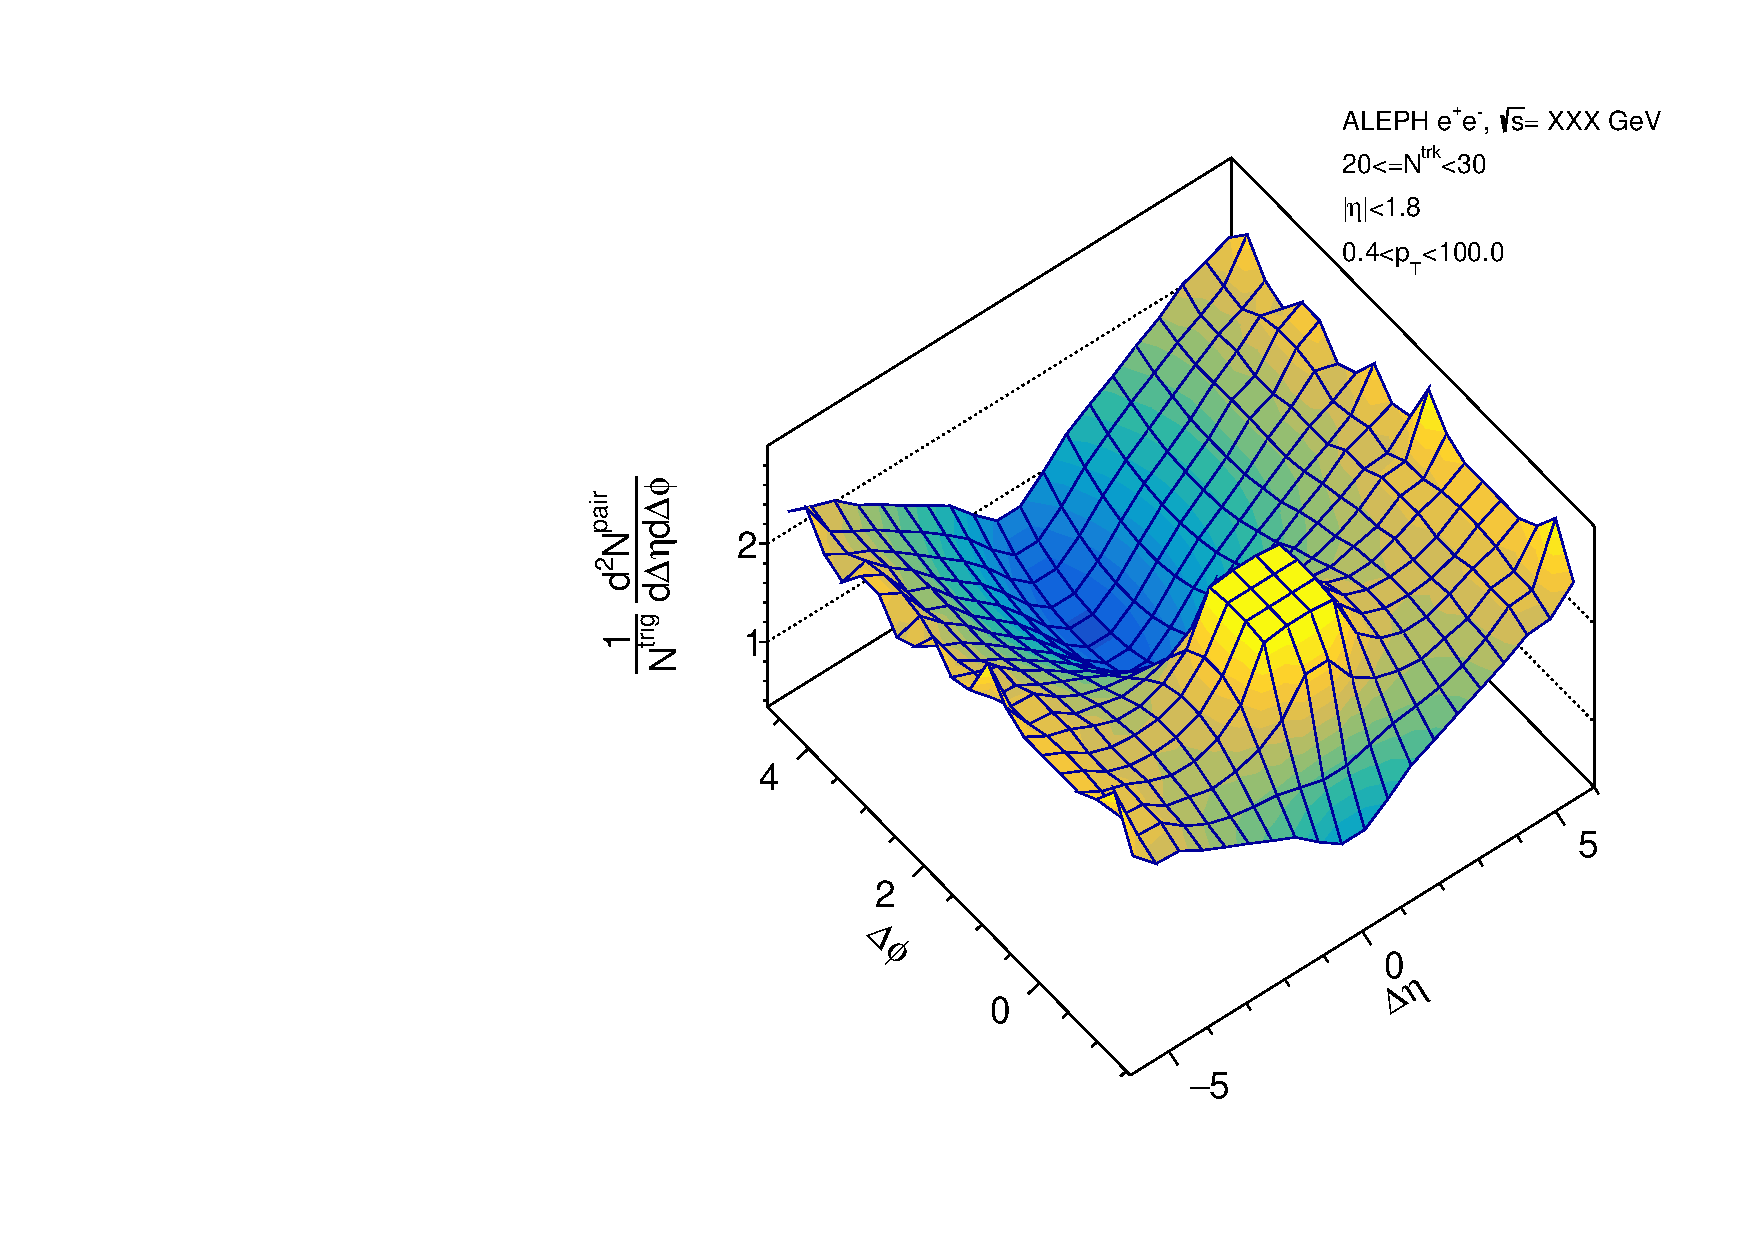
\includegraphics[width=.32\textwidth]{images/TwoParticleCorrelation/LEP1_WTA/LEP1_WTA_ratio2_20_30.pdf}}\hfill
\subfloat{\label{sfig:e}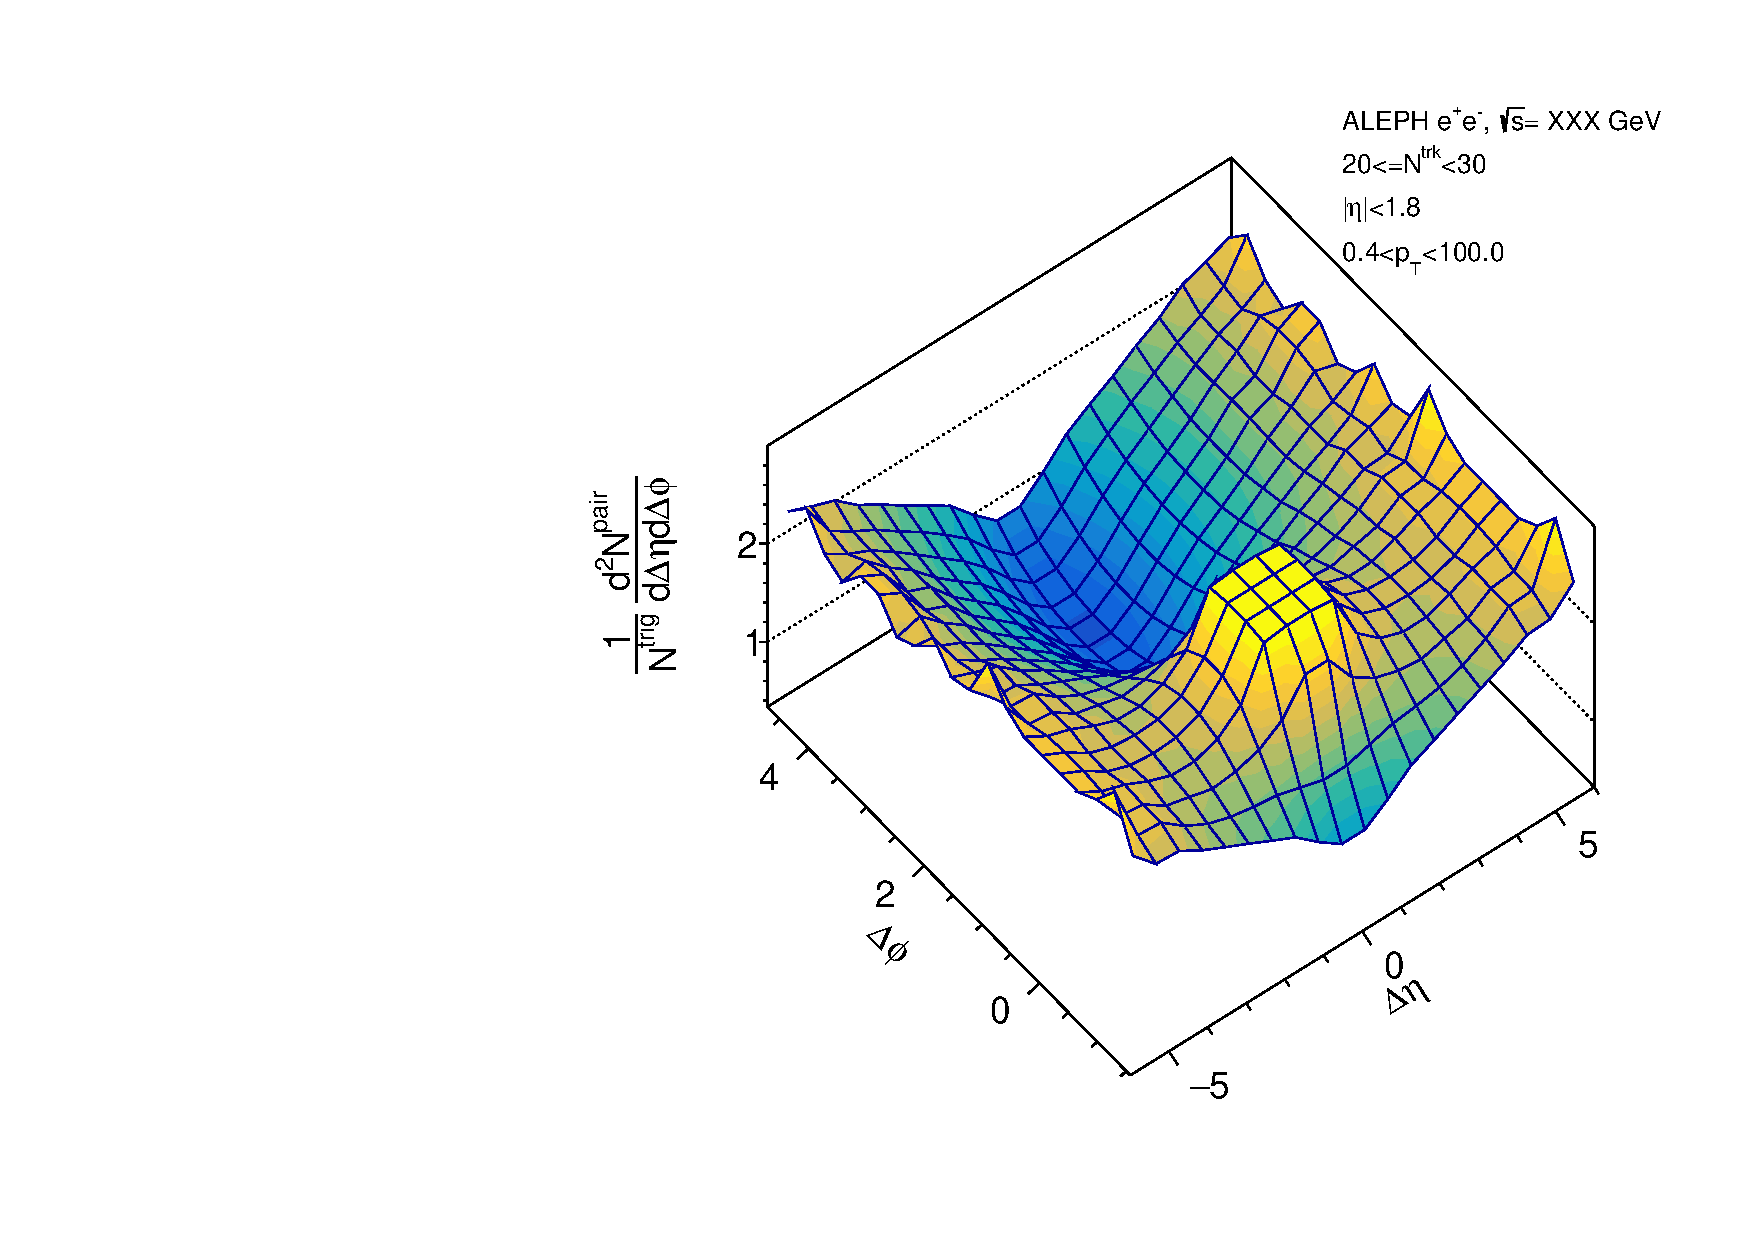
\includegraphics[width=.32\textwidth]{images/TwoParticleCorrelation/LEP1_WTA/LEP1_WTA_ratio1_20_30.pdf}}\hfill
\subfloat{\label{sfig:f}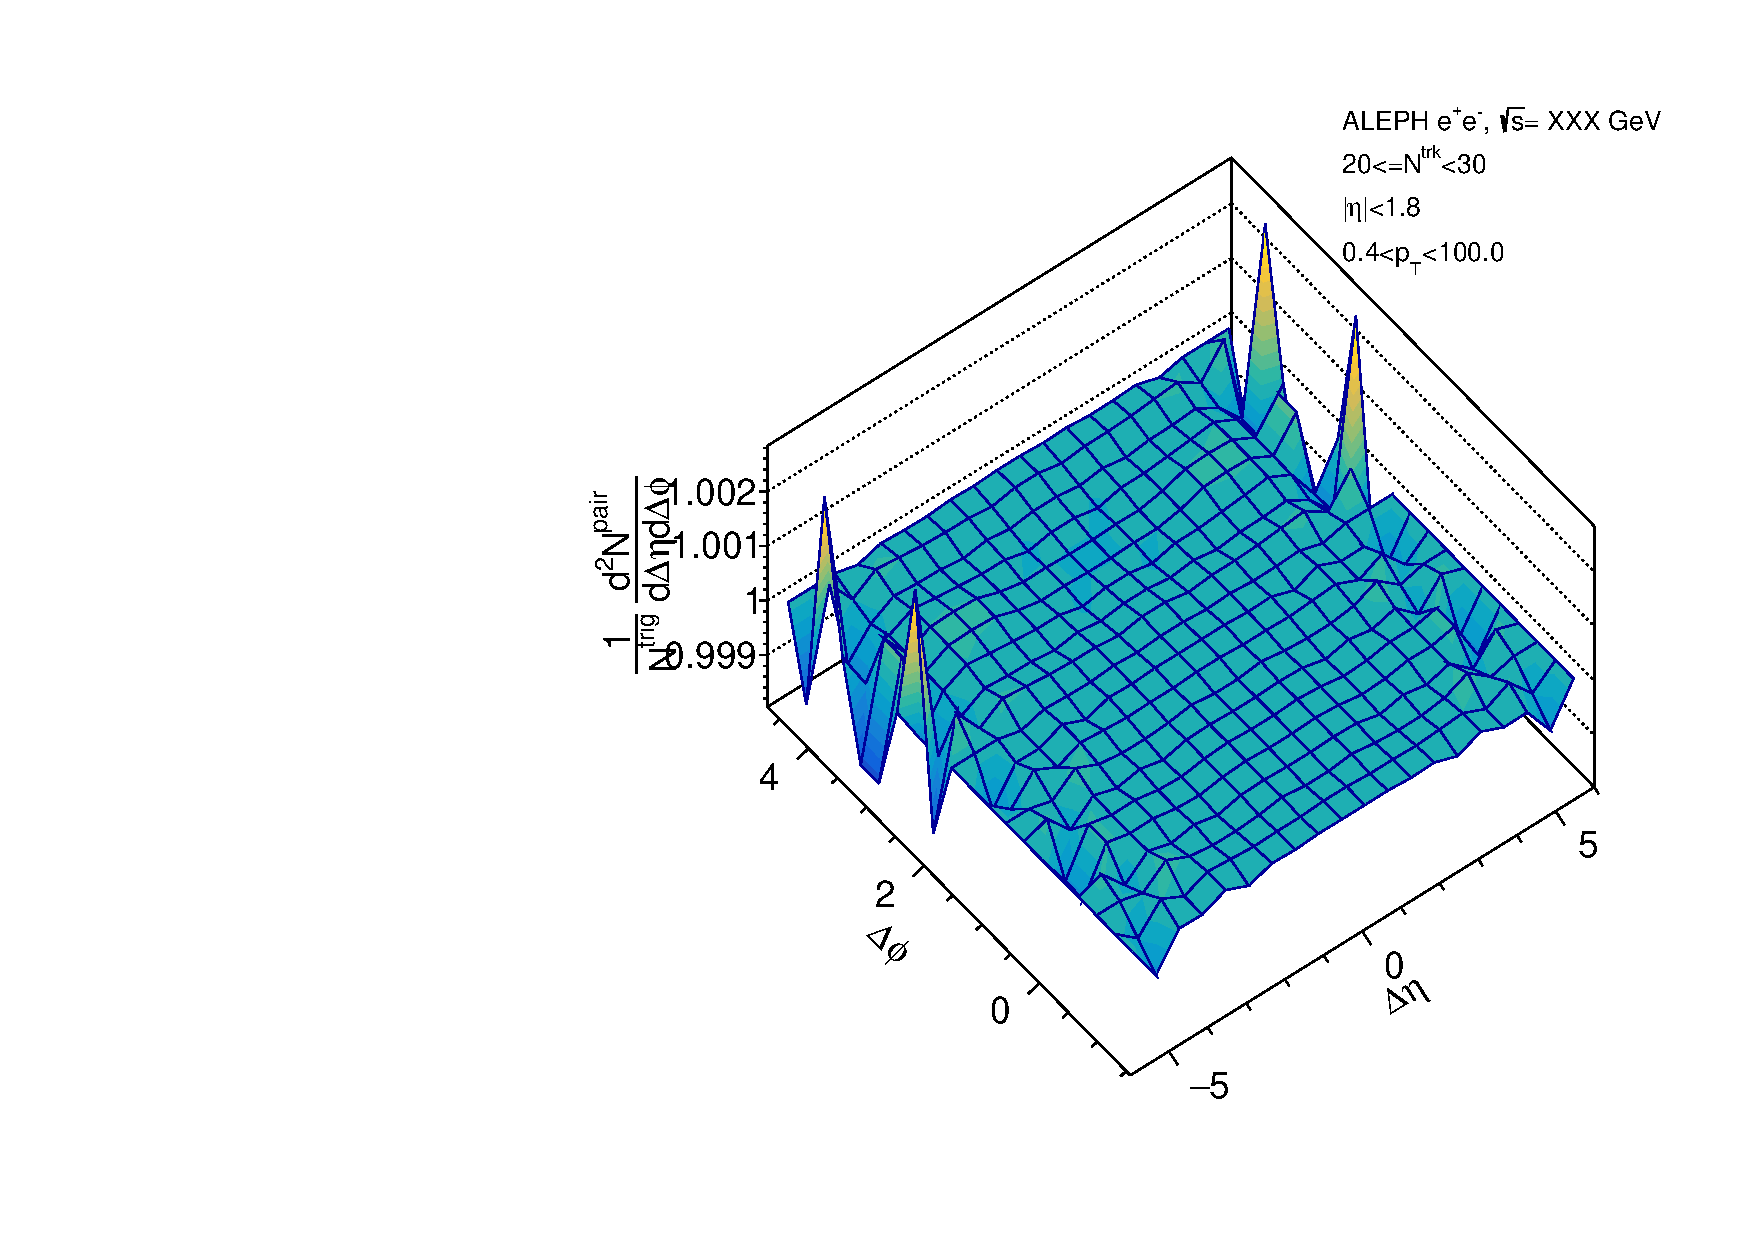
\includegraphics[width=.32\textwidth]{images/TwoParticleCorrelation/LEP1_WTA/LEP1_WTA_r_ratio_20_30.pdf}}\hfill
\subfloat{\label{sfig:g}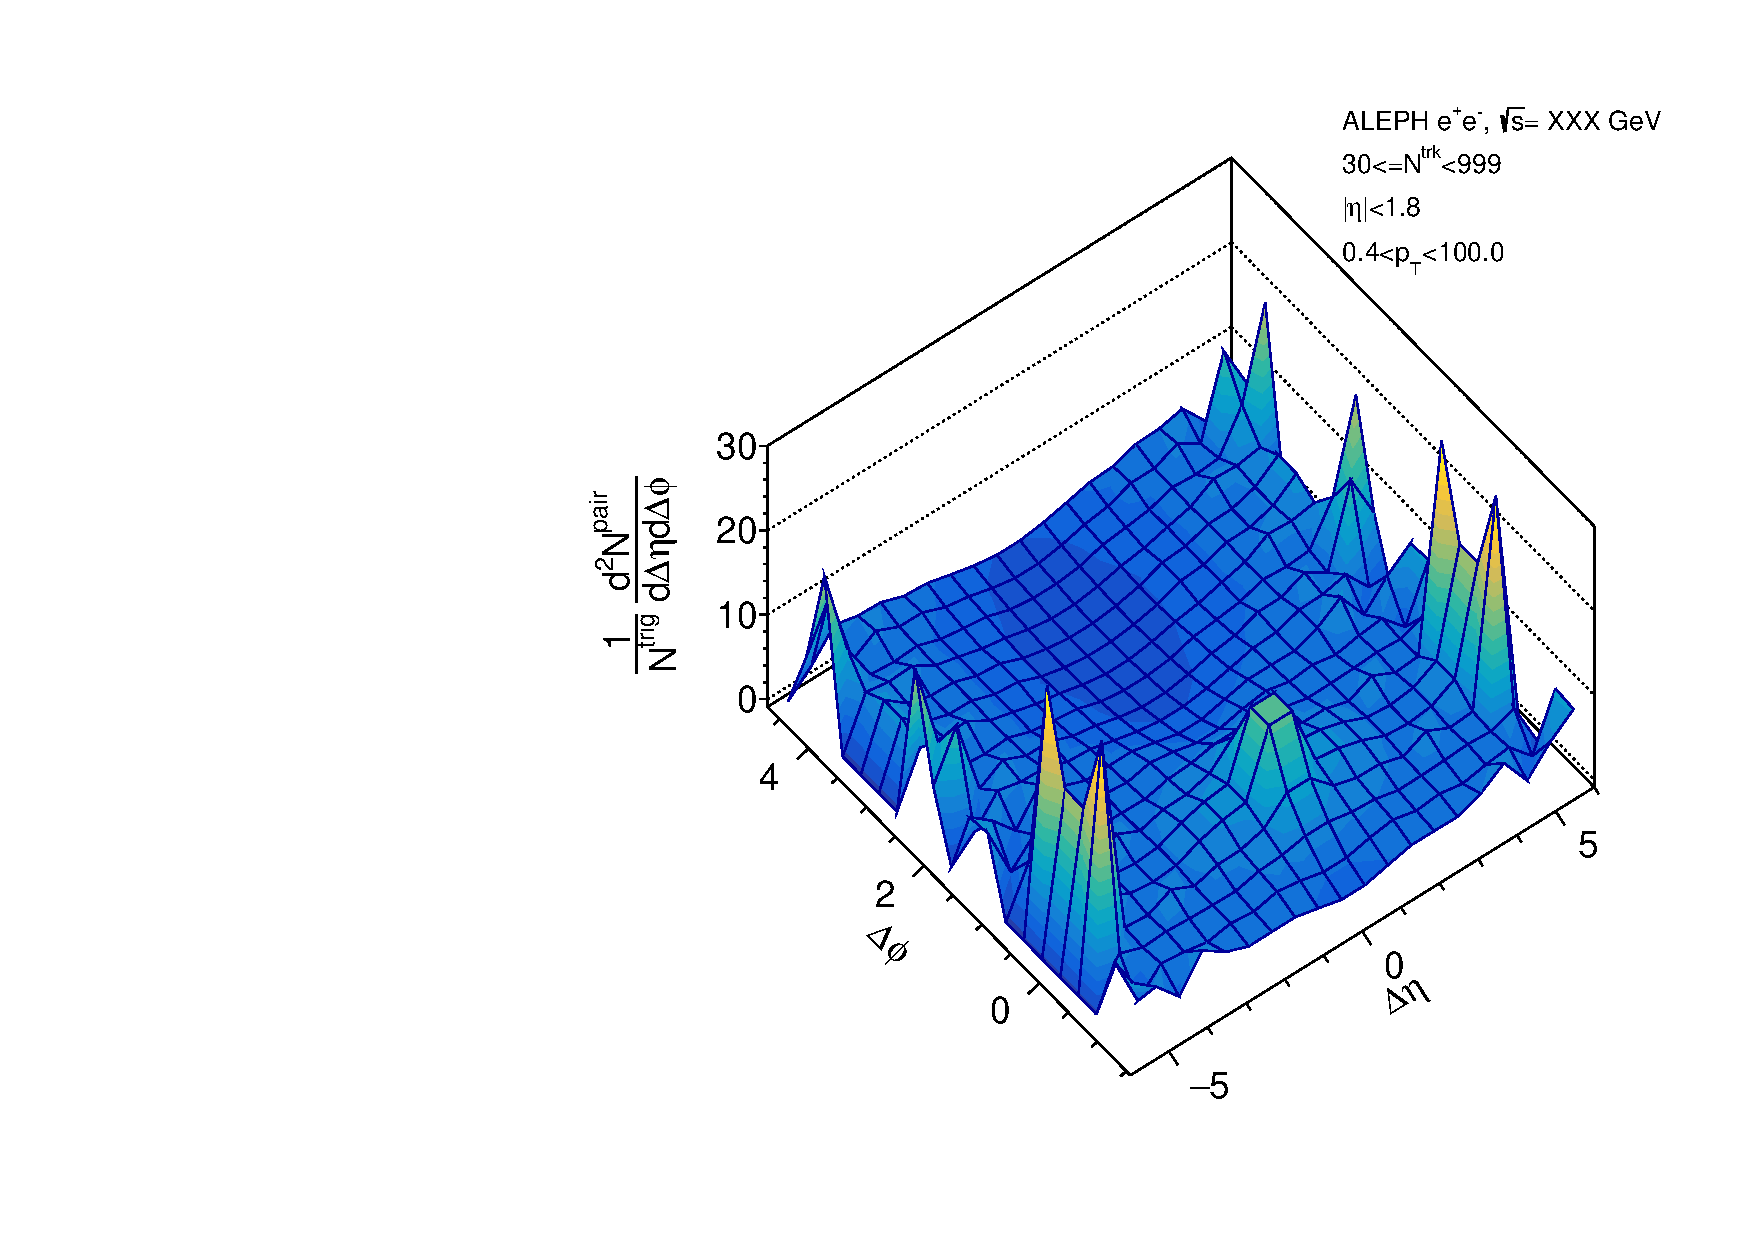
\includegraphics[width=.32\textwidth]{images/TwoParticleCorrelation/LEP1_WTA/LEP1_WTA_ratio2_30_999.pdf}}\hfill
\subfloat{\label{sfig:h}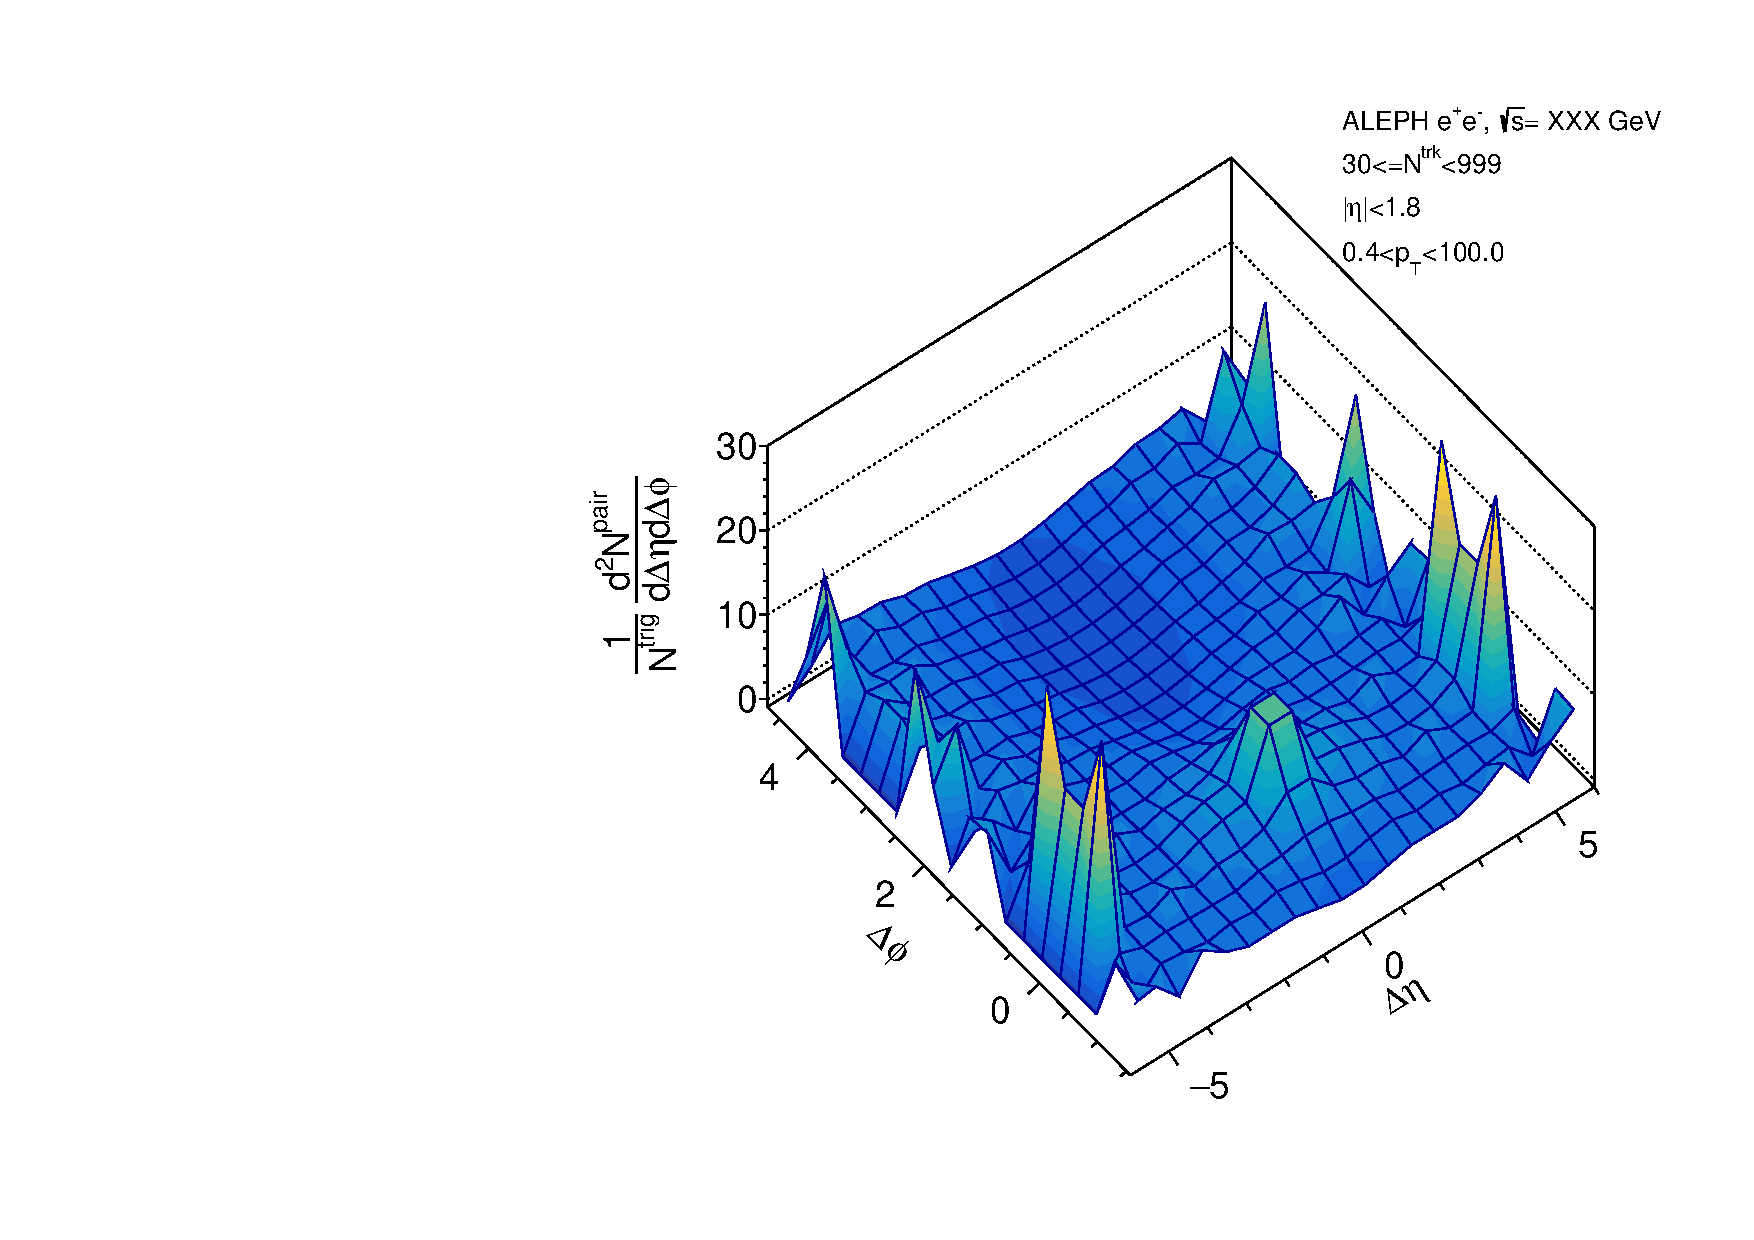
\includegraphics[width=.32\textwidth]{images/TwoParticleCorrelation/LEP1_WTA/LEP1_WTA_ratio1_30_999.pdf}}\hfill
\subfloat{\label{sfig:i}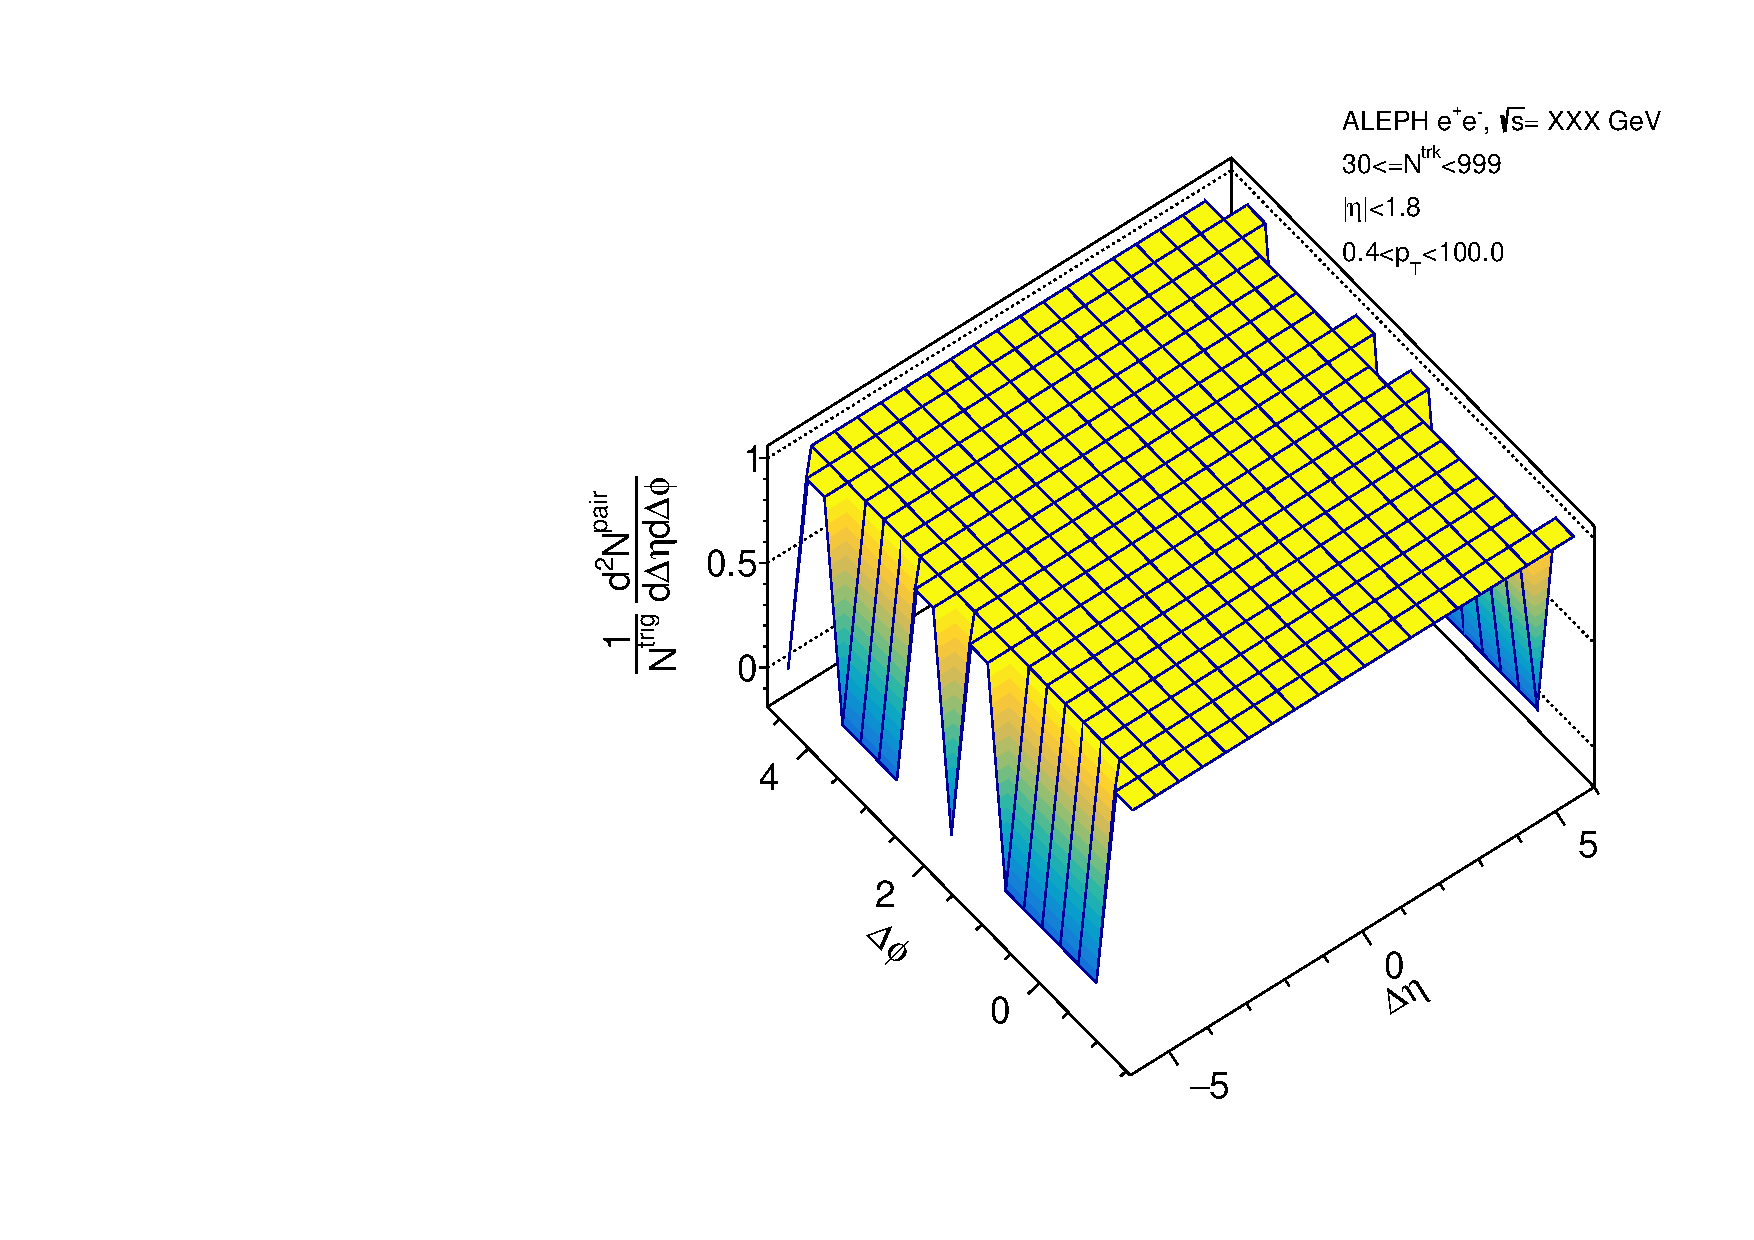
\includegraphics[width=.32\textwidth]{images/TwoParticleCorrelation/LEP1_WTA/LEP1_WTA_r_ratio_30_999.pdf}} \\
\caption{Two particle correlation fuctions for the LEP1 data set analyzed in the WTA axis.}
\label{fig:test}
\end{figure}

%%%%%%%%%%% LEP2 %%%%%%%%%%%
\begin{figure}[h!]
\centering
\subfloat{\label{sfig:a}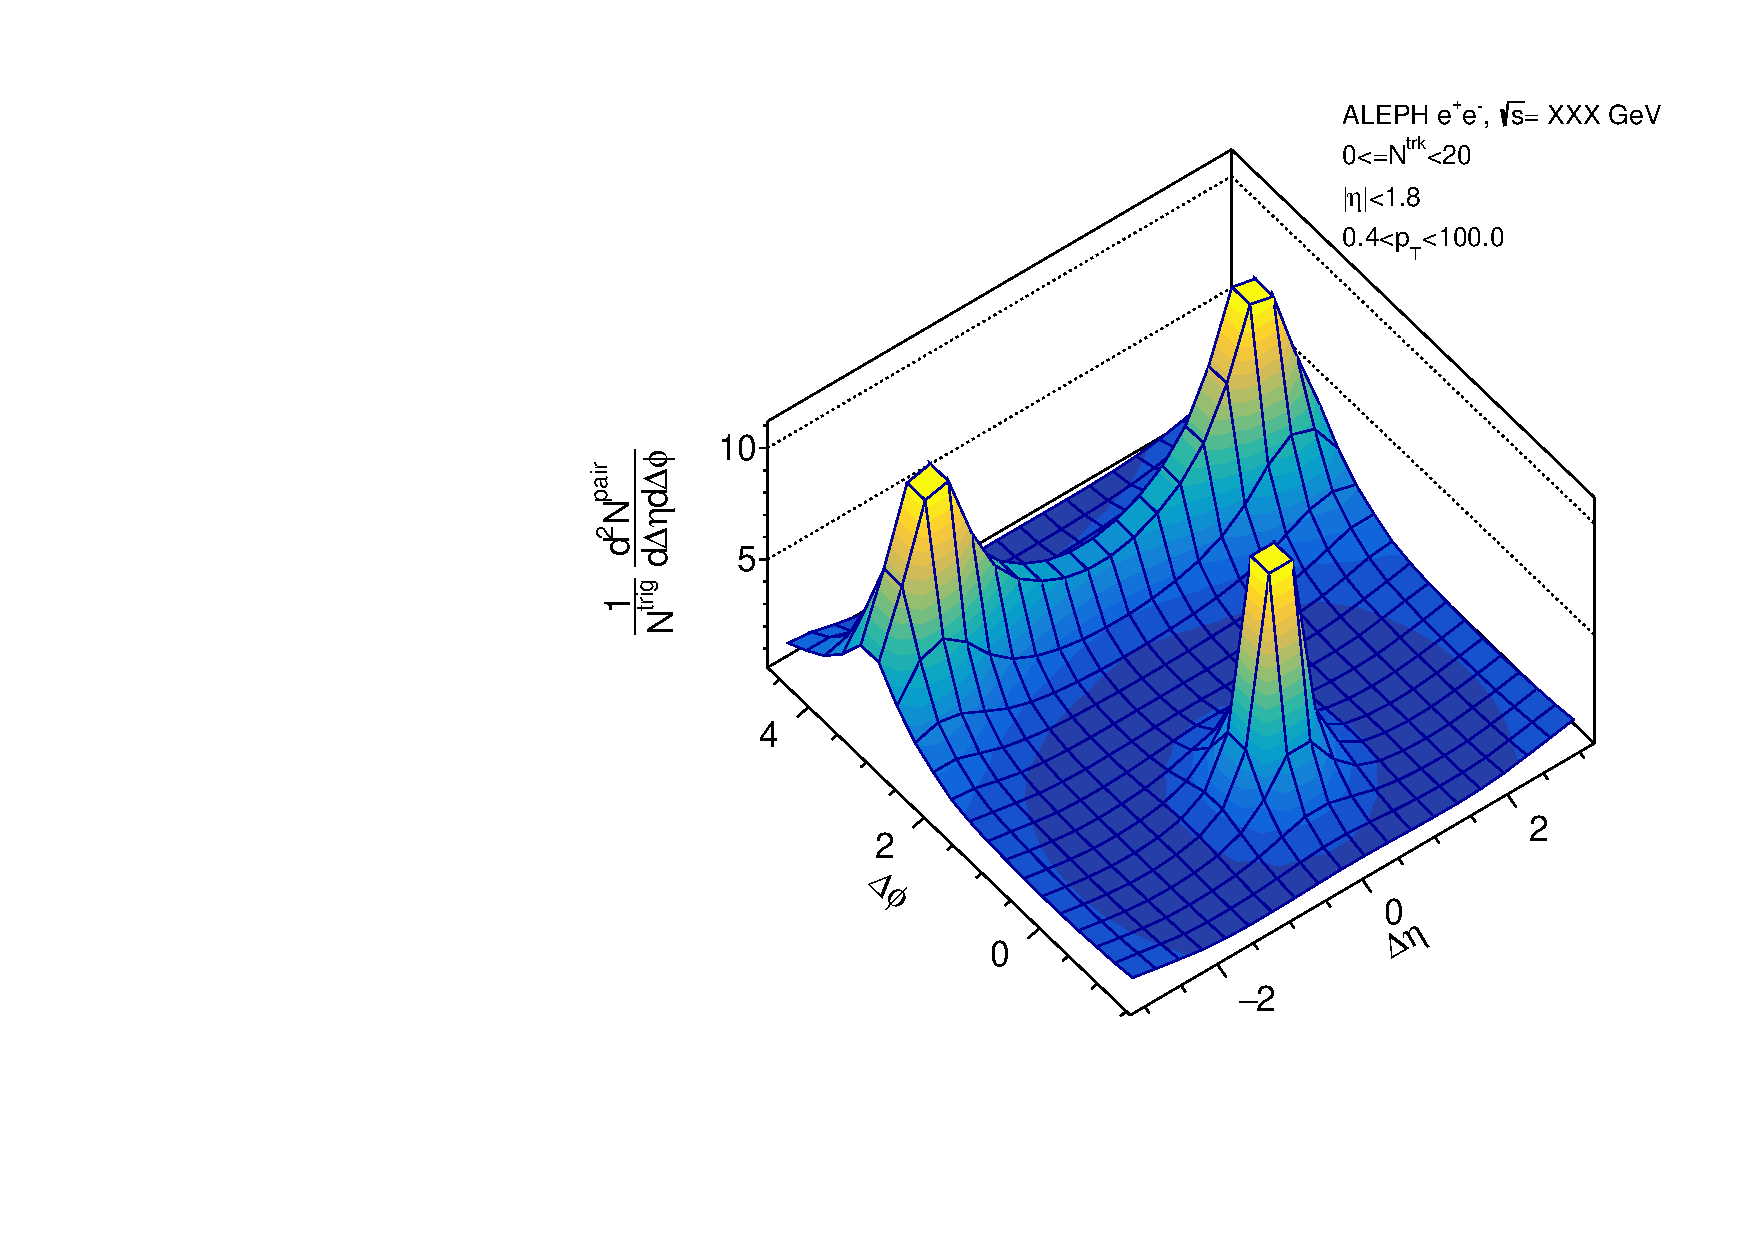
\includegraphics[width=.32\textwidth]{images/TwoParticleCorrelation/LEP2_BEAM/LEP2_BEAM_ratio2_0_20.pdf}}\hfill
\subfloat{\label{sfig:b}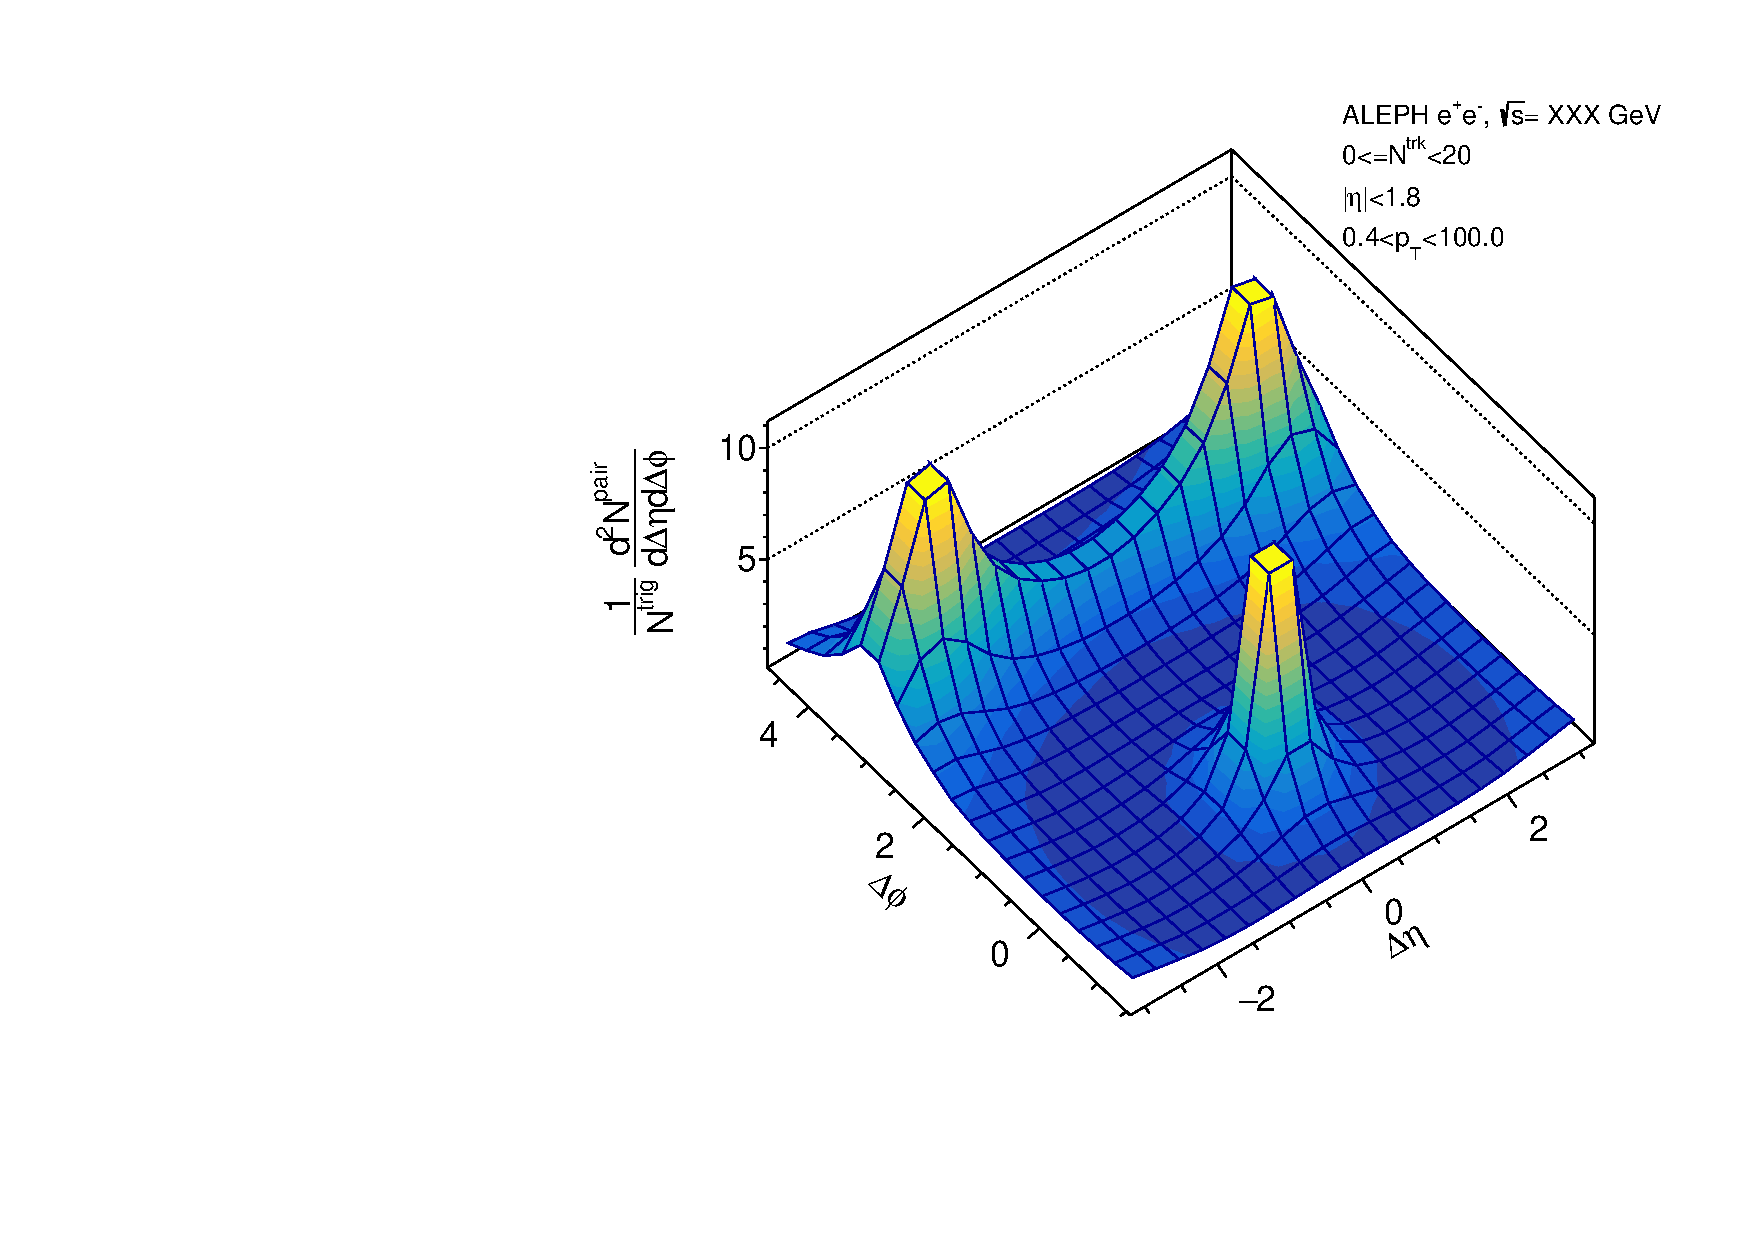
\includegraphics[width=.32\textwidth]{images/TwoParticleCorrelation/LEP2_BEAM/LEP2_BEAM_ratio1_0_20.pdf}}\hfill
\subfloat{\label{sfig:c}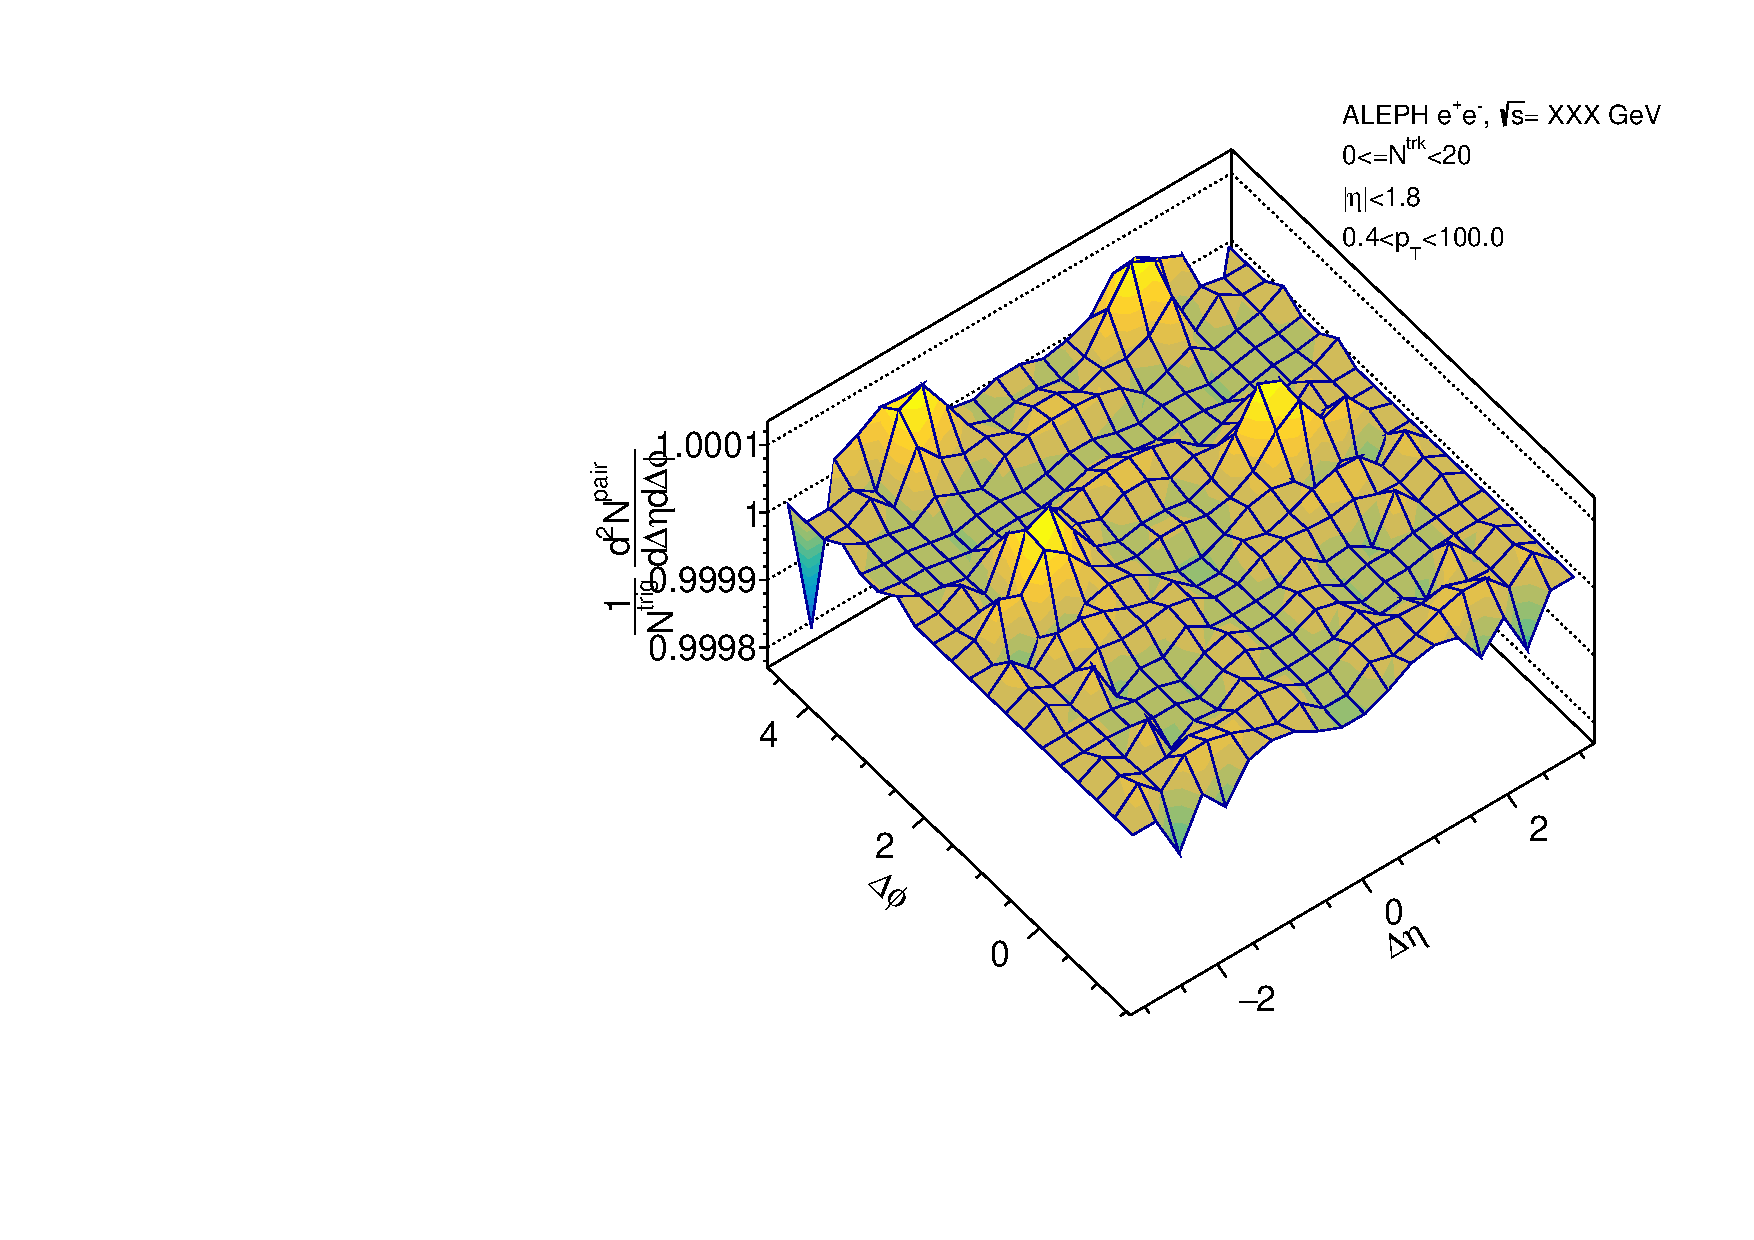
\includegraphics[width=.32\textwidth]{images/TwoParticleCorrelation/LEP2_BEAM/LEP2_BEAM_r_ratio_0_20.pdf}}\hfill
\subfloat{\label{sfig:d}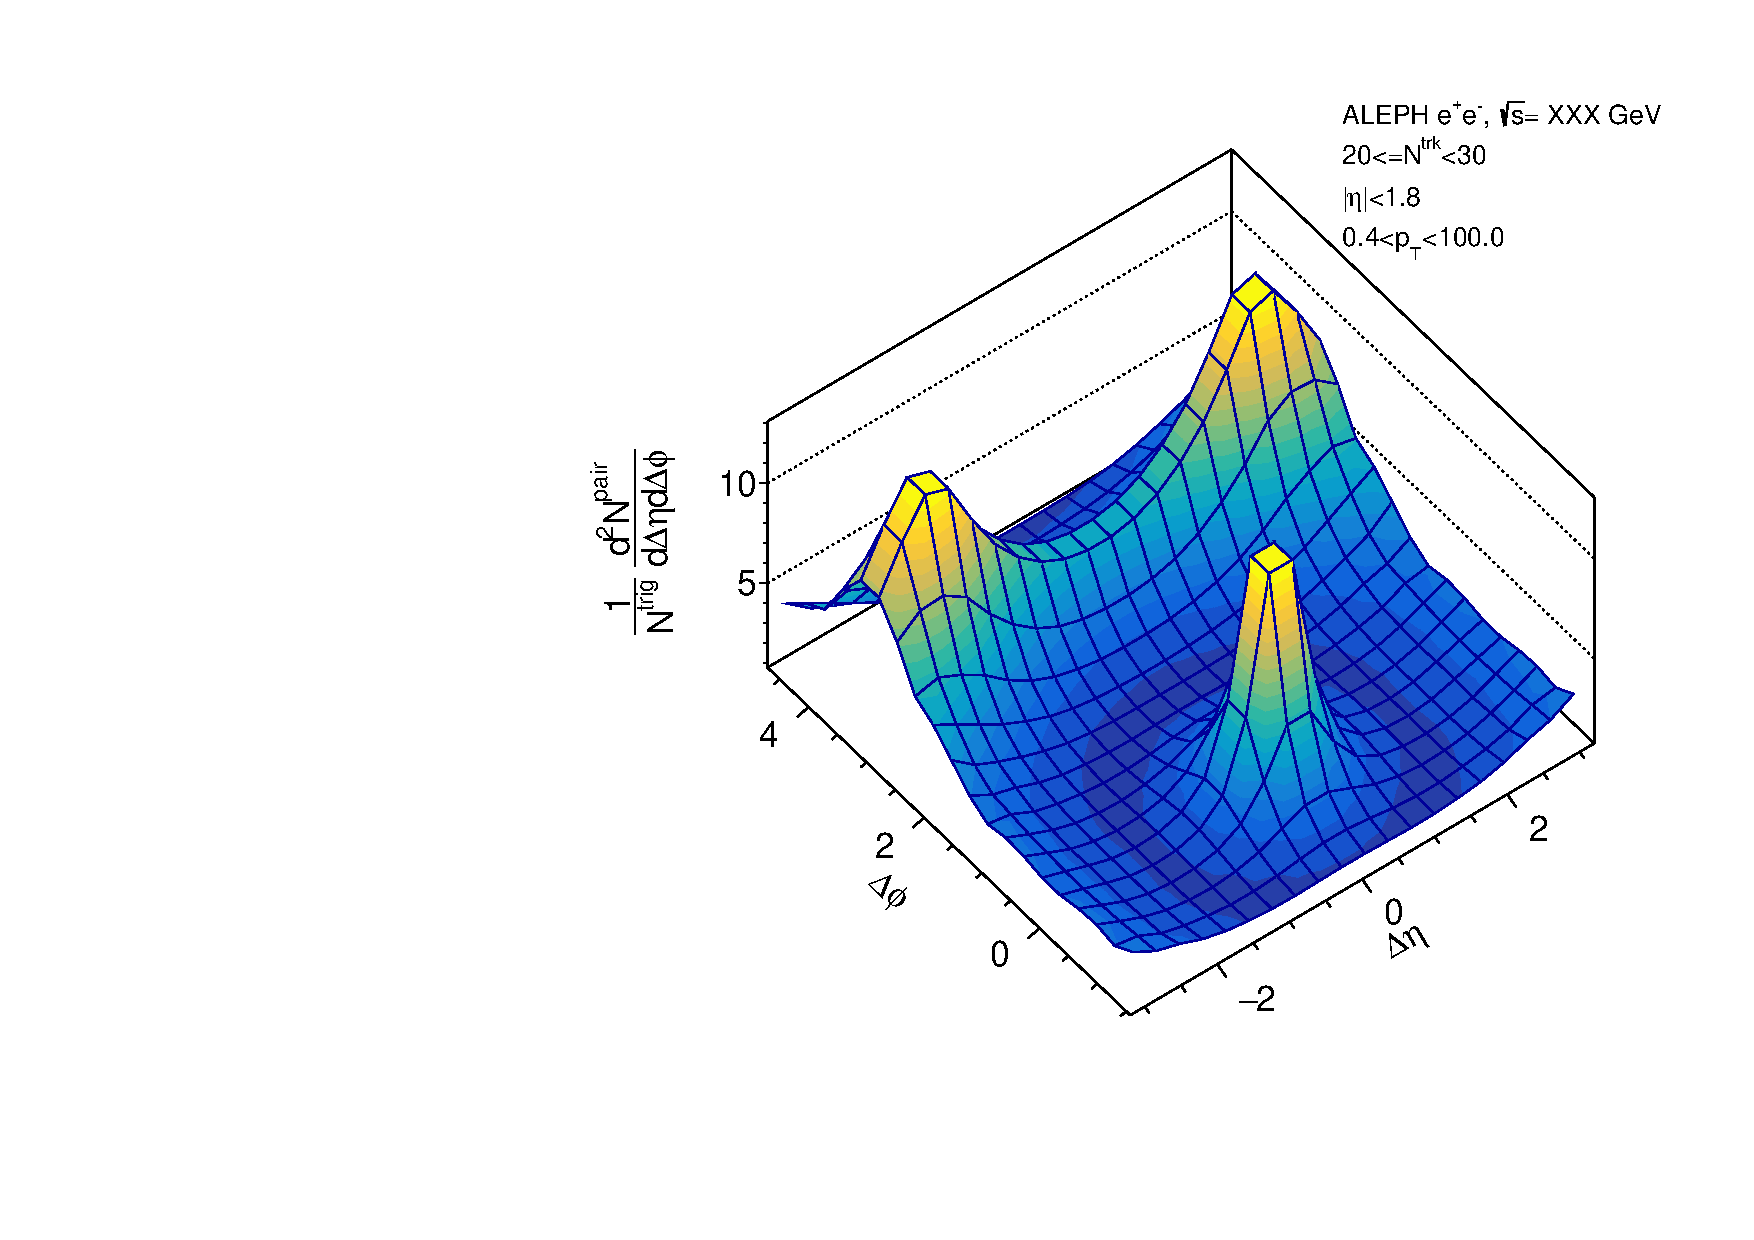
\includegraphics[width=.32\textwidth]{images/TwoParticleCorrelation/LEP2_BEAM/LEP2_BEAM_ratio2_20_30.pdf}}\hfill
\subfloat{\label{sfig:e}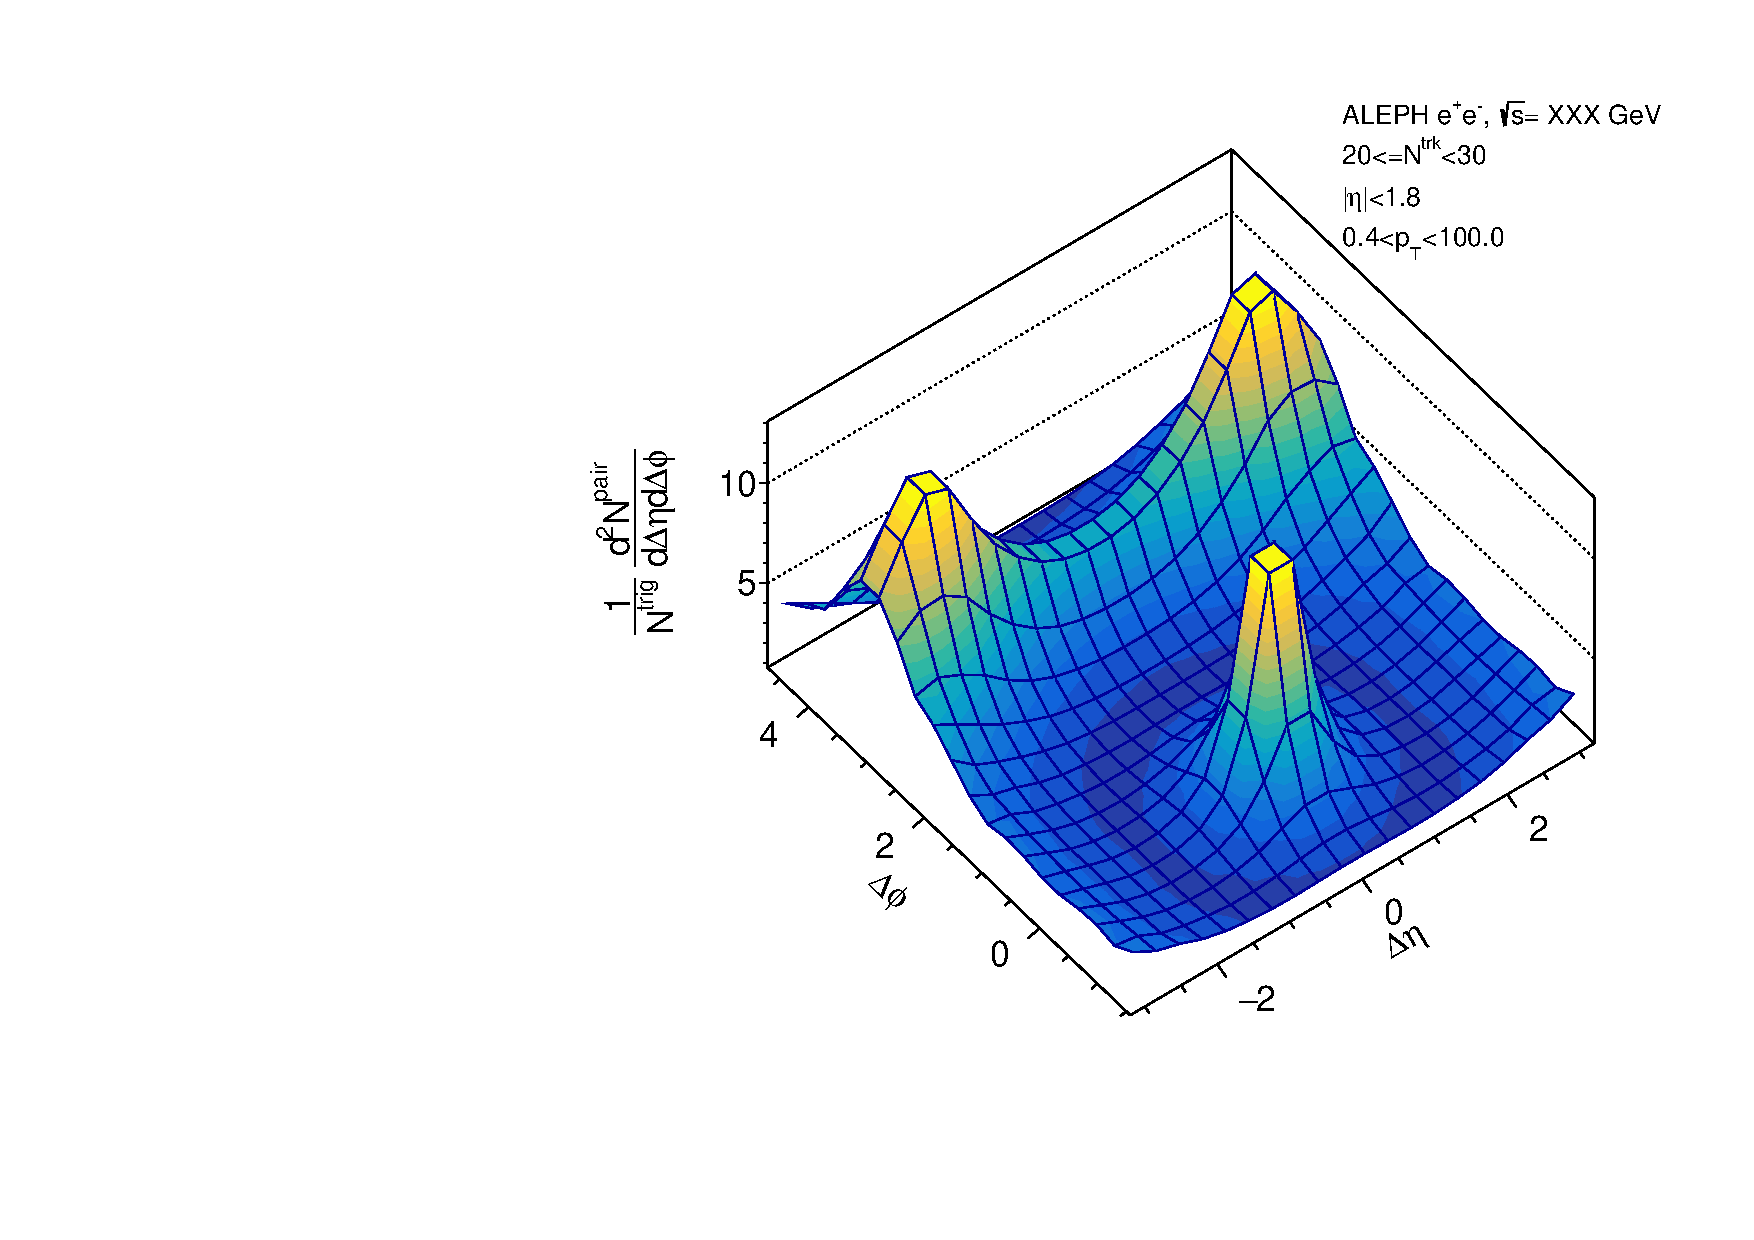
\includegraphics[width=.32\textwidth]{images/TwoParticleCorrelation/LEP2_BEAM/LEP2_BEAM_ratio1_20_30.pdf}}\hfill
\subfloat{\label{sfig:f}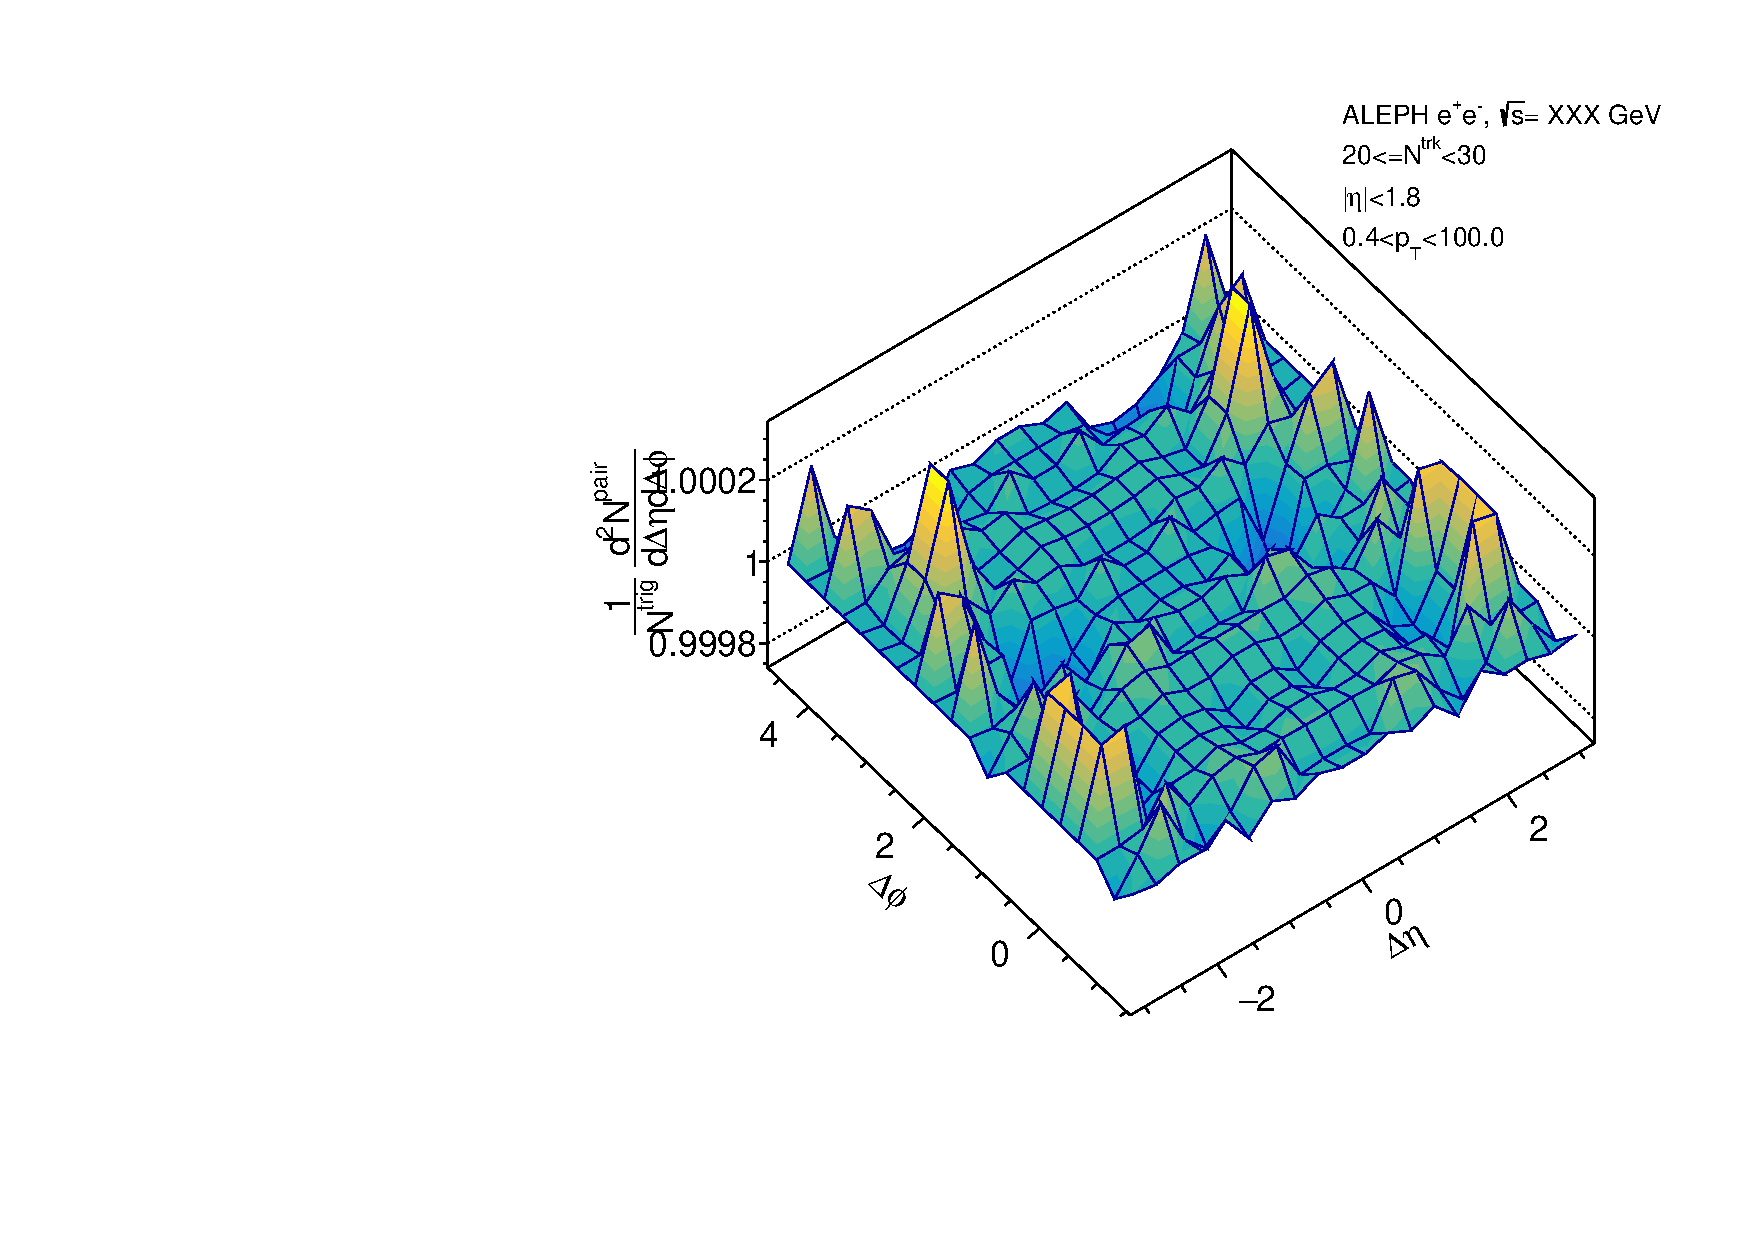
\includegraphics[width=.32\textwidth]{images/TwoParticleCorrelation/LEP2_BEAM/LEP2_BEAM_r_ratio_20_30.pdf}}\hfill
\subfloat{\label{sfig:g}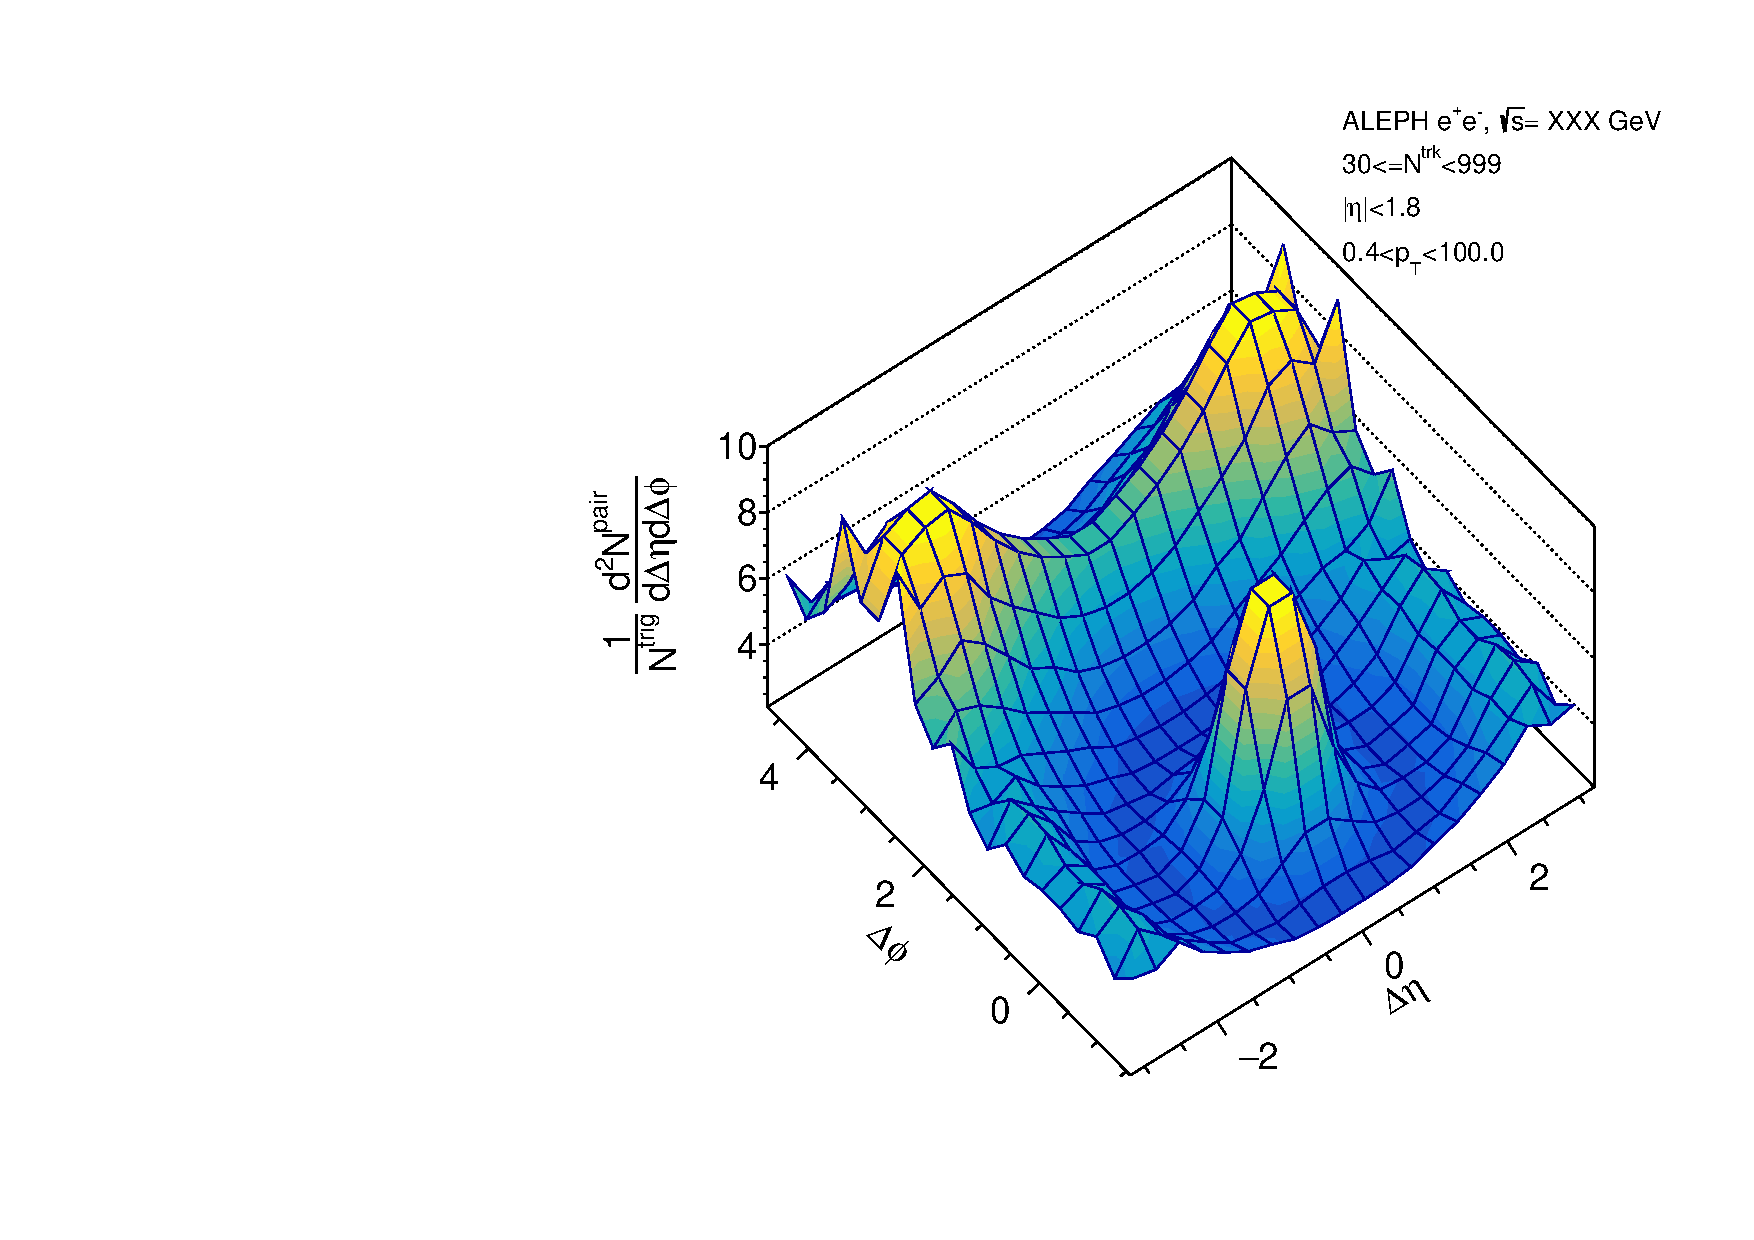
\includegraphics[width=.32\textwidth]{images/TwoParticleCorrelation/LEP2_BEAM/LEP2_BEAM_ratio2_30_999.pdf}}\hfill
\subfloat{\label{sfig:h}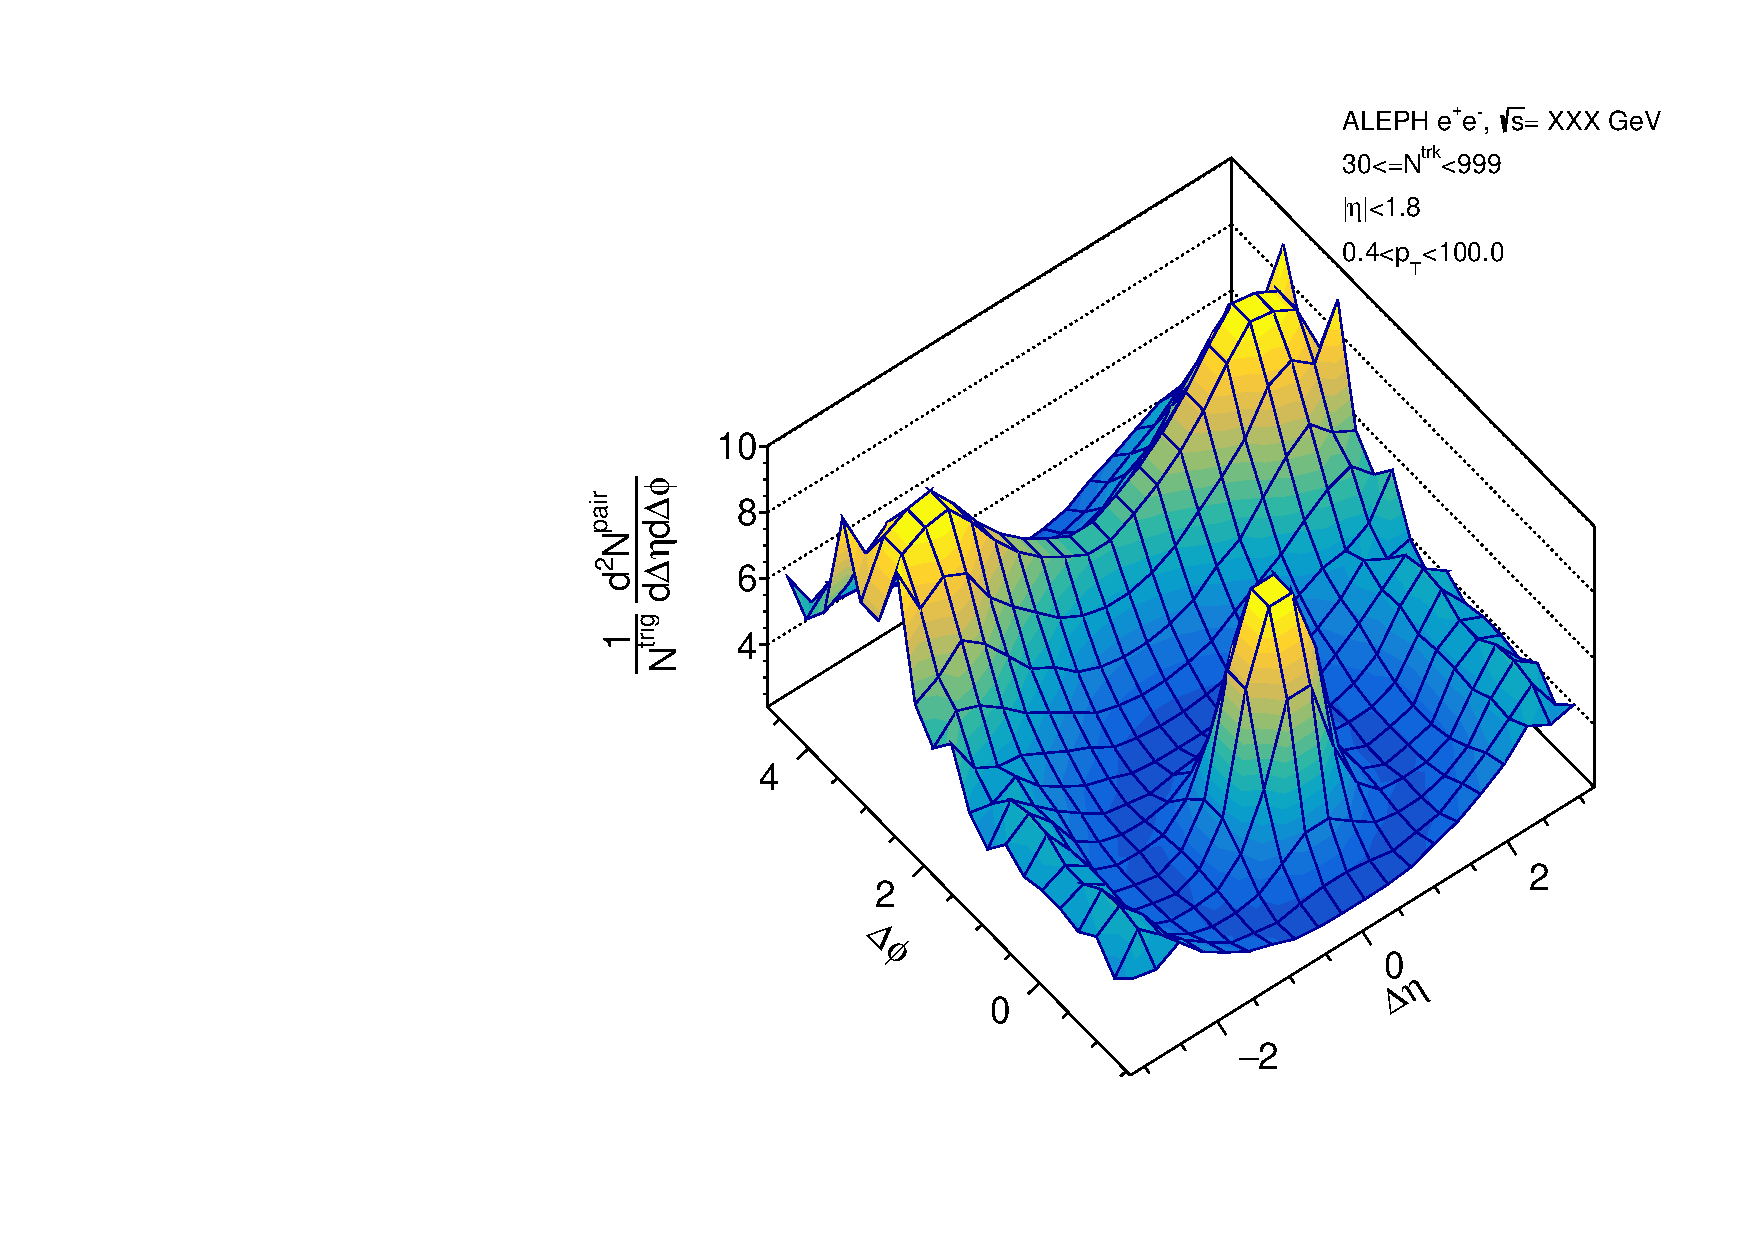
\includegraphics[width=.32\textwidth]{images/TwoParticleCorrelation/LEP2_BEAM/LEP2_BEAM_ratio1_30_999.pdf}}\hfill
\subfloat{\label{sfig:i}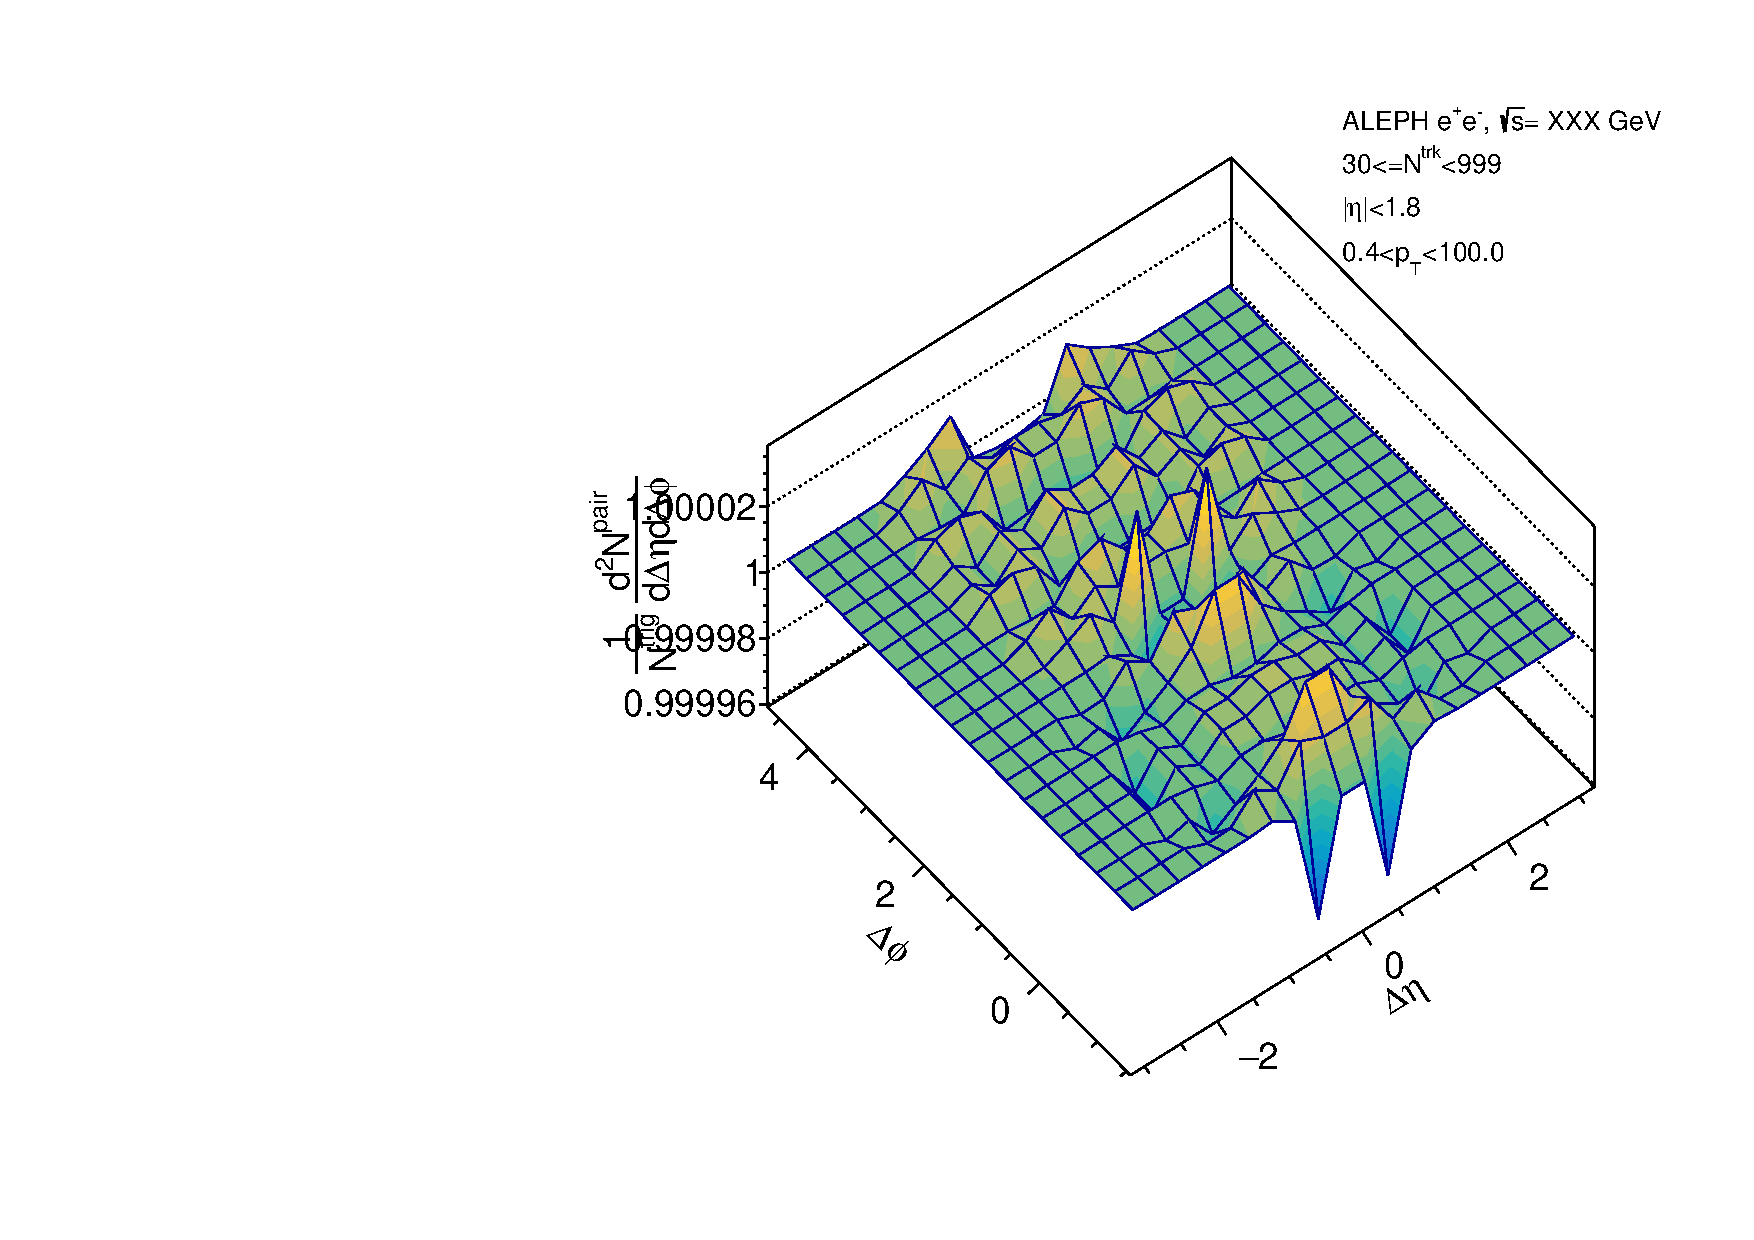
\includegraphics[width=.32\textwidth]{images/TwoParticleCorrelation/LEP2_BEAM/LEP2_BEAM_r_ratio_30_999.pdf}} \\
\caption{Two particle correlation fuctions for the LEP2 data set analyzed in the beam axis.}
\label{fig:test}
\end{figure}

\begin{figure}[h!]
\centering
\subfloat{\label{sfig:a}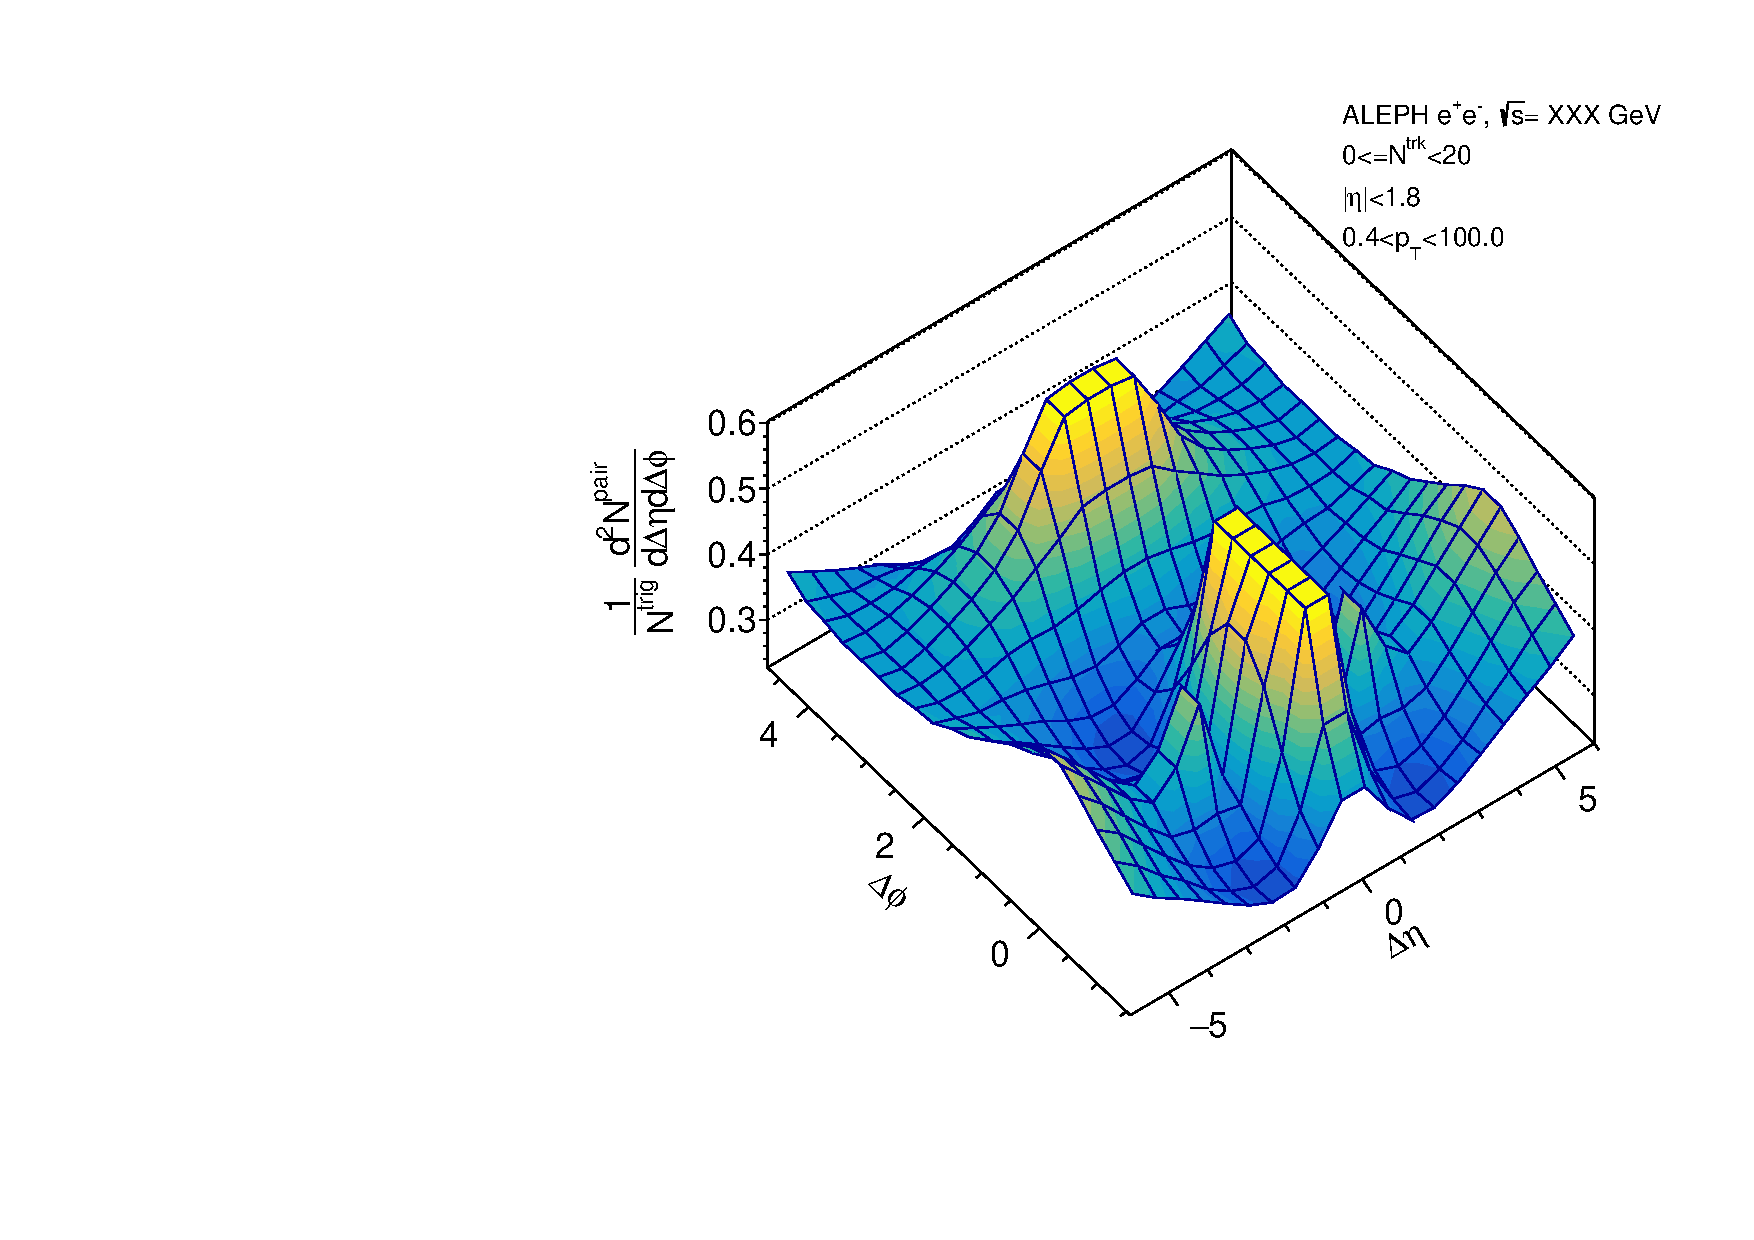
\includegraphics[width=.32\textwidth]{images/TwoParticleCorrelation/LEP2_THRUST/LEP2_THRUST_ratio2_0_20.pdf}}\hfill
\subfloat{\label{sfig:b}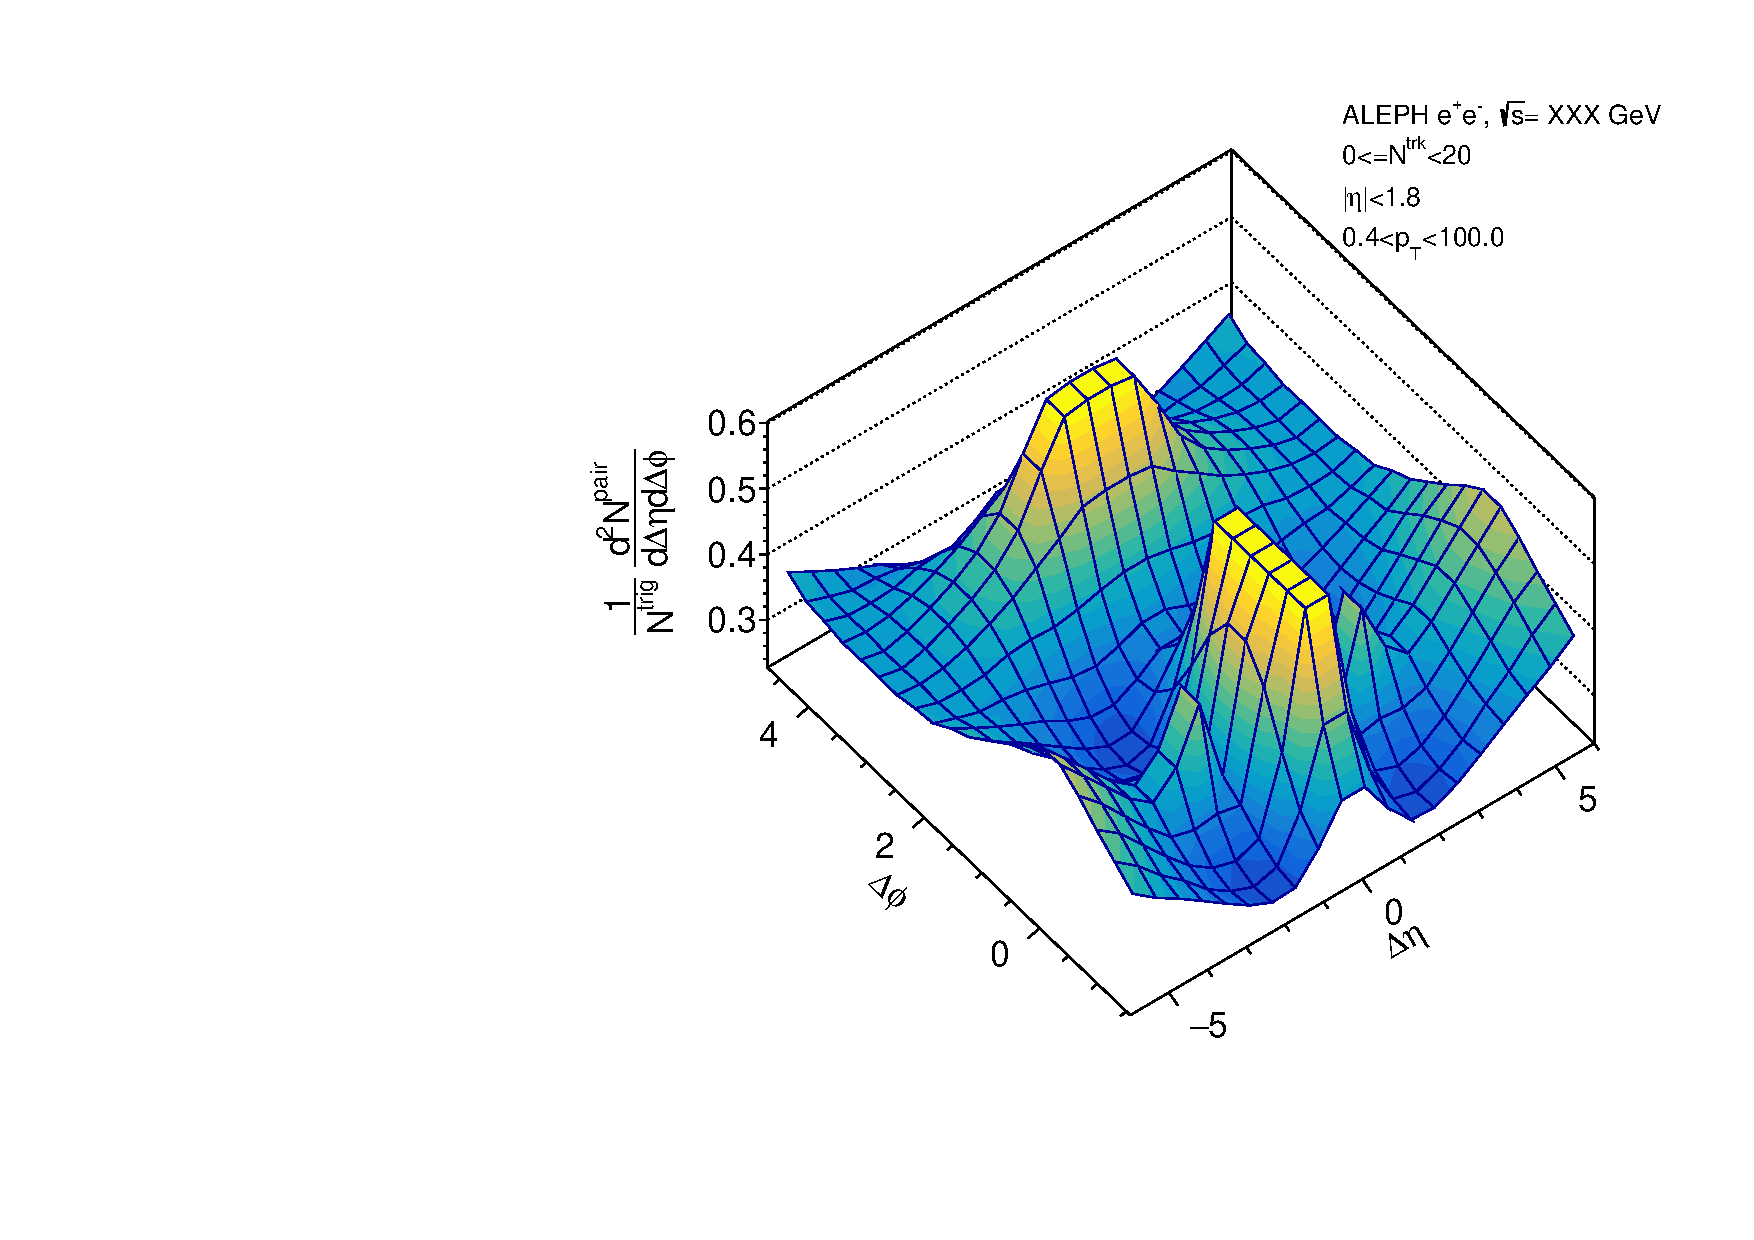
\includegraphics[width=.32\textwidth]{images/TwoParticleCorrelation/LEP2_THRUST/LEP2_THRUST_ratio1_0_20.pdf}}\hfill
\subfloat{\label{sfig:c}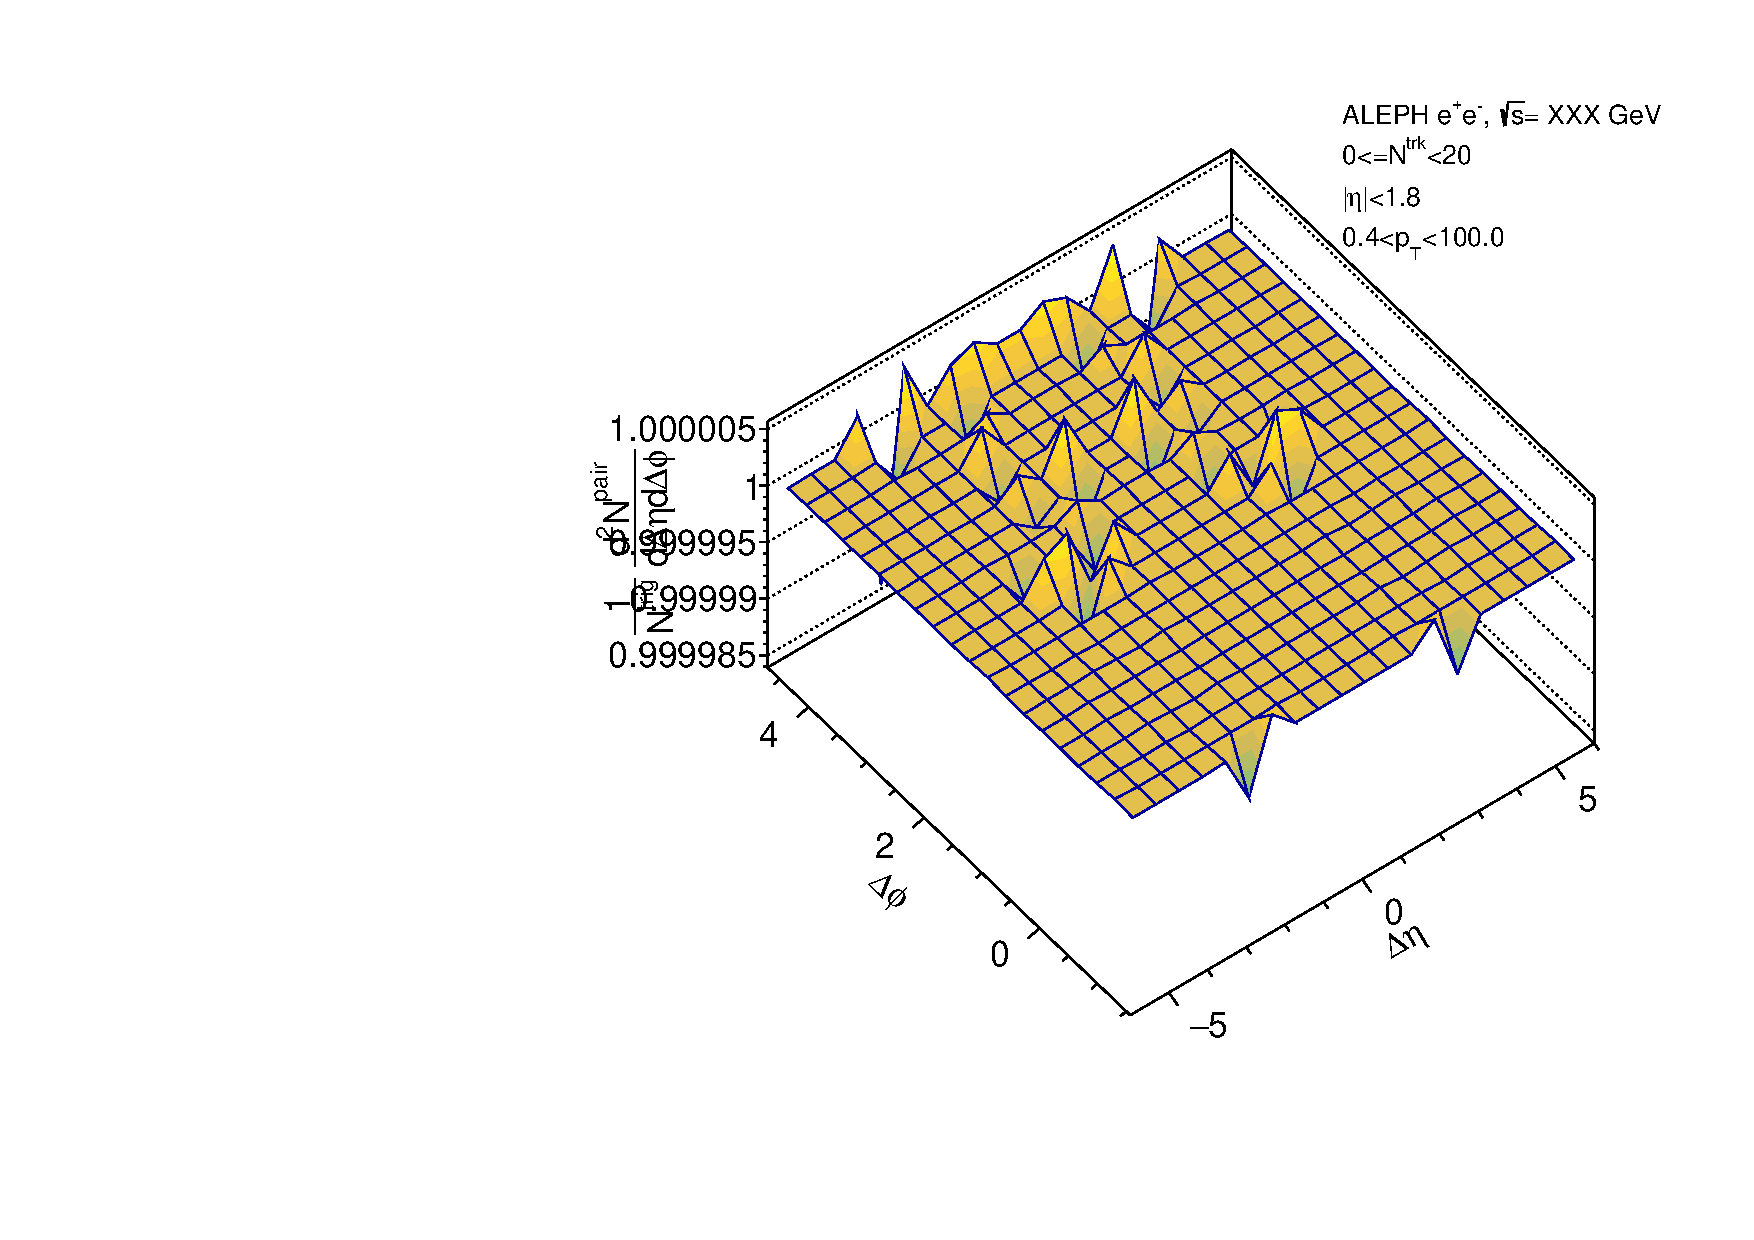
\includegraphics[width=.32\textwidth]{images/TwoParticleCorrelation/LEP2_THRUST/LEP2_THRUST_r_ratio_0_20.pdf}}\hfill
\subfloat{\label{sfig:d}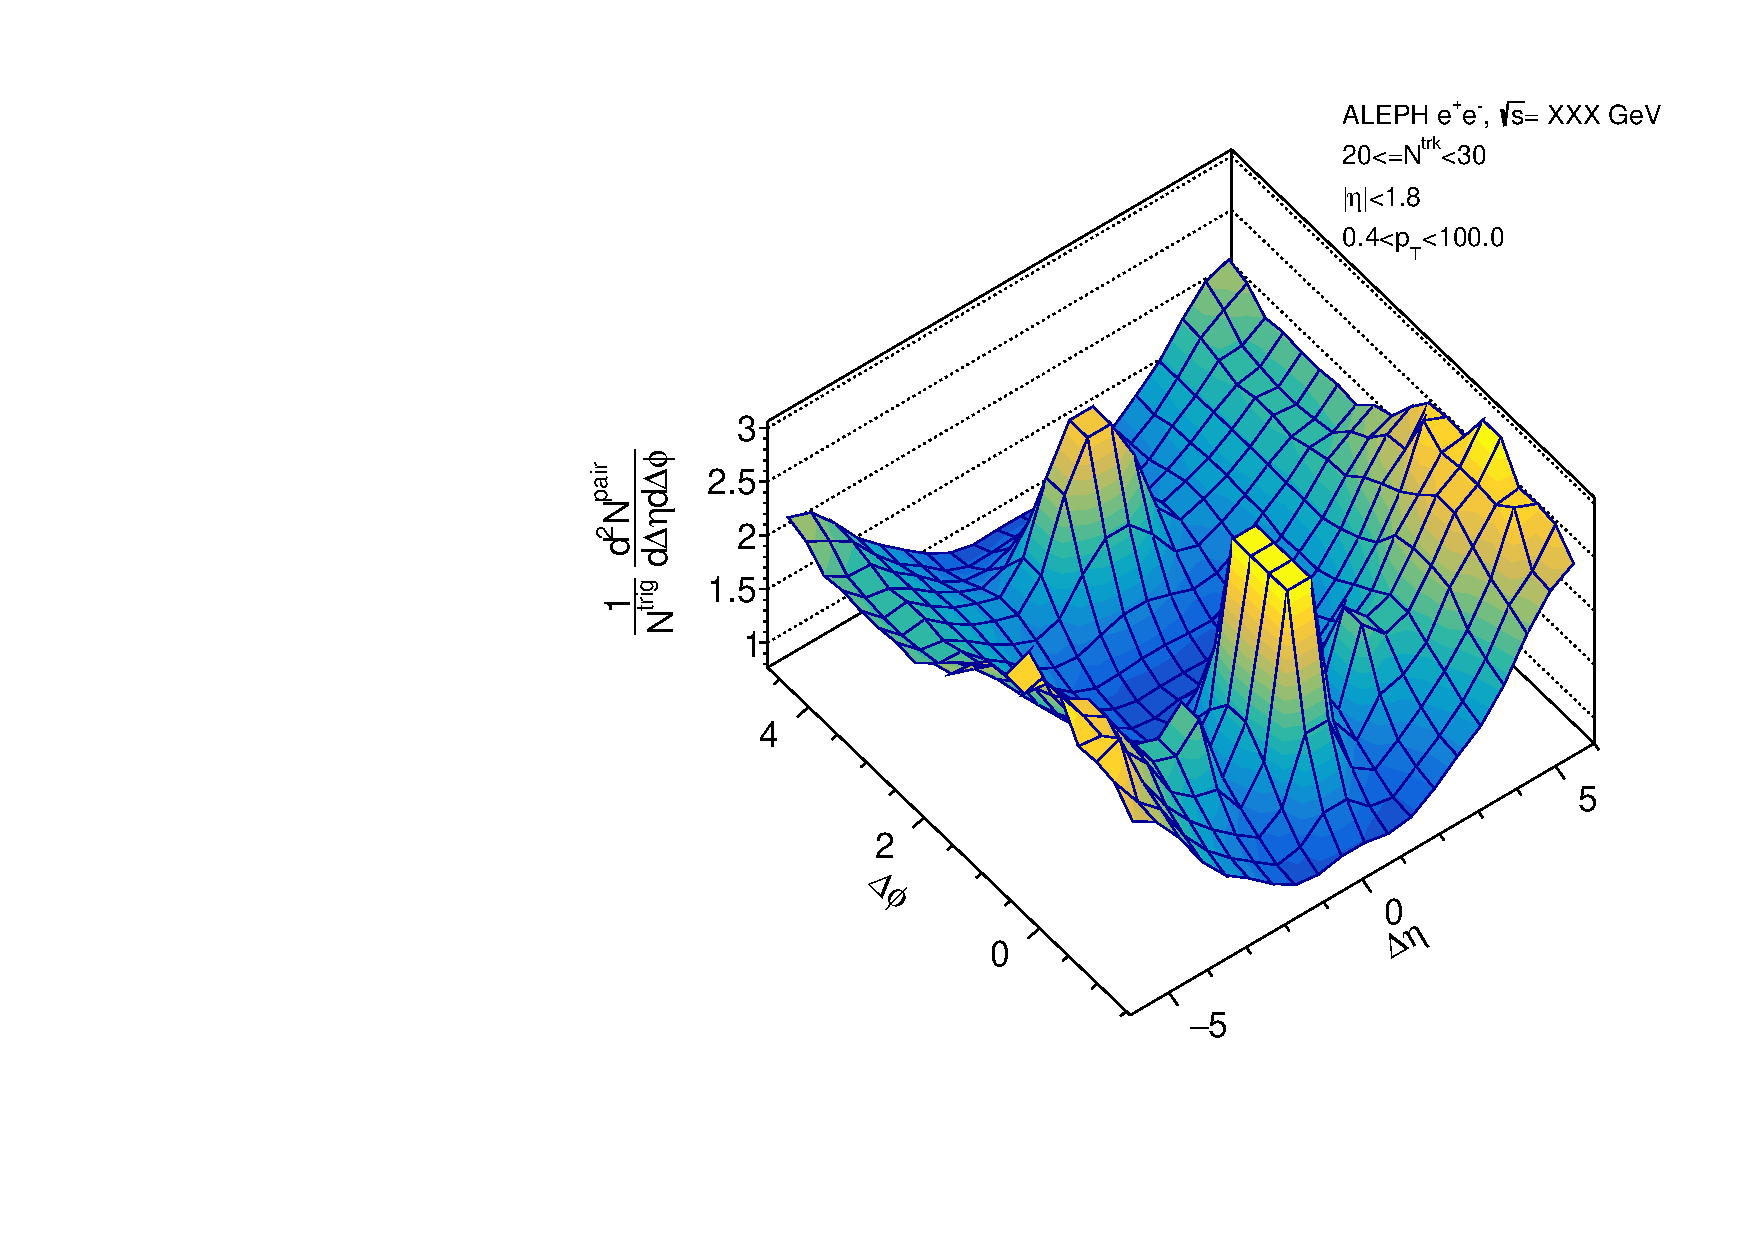
\includegraphics[width=.32\textwidth]{images/TwoParticleCorrelation/LEP2_THRUST/LEP2_THRUST_ratio2_20_30.pdf}}\hfill
\subfloat{\label{sfig:e}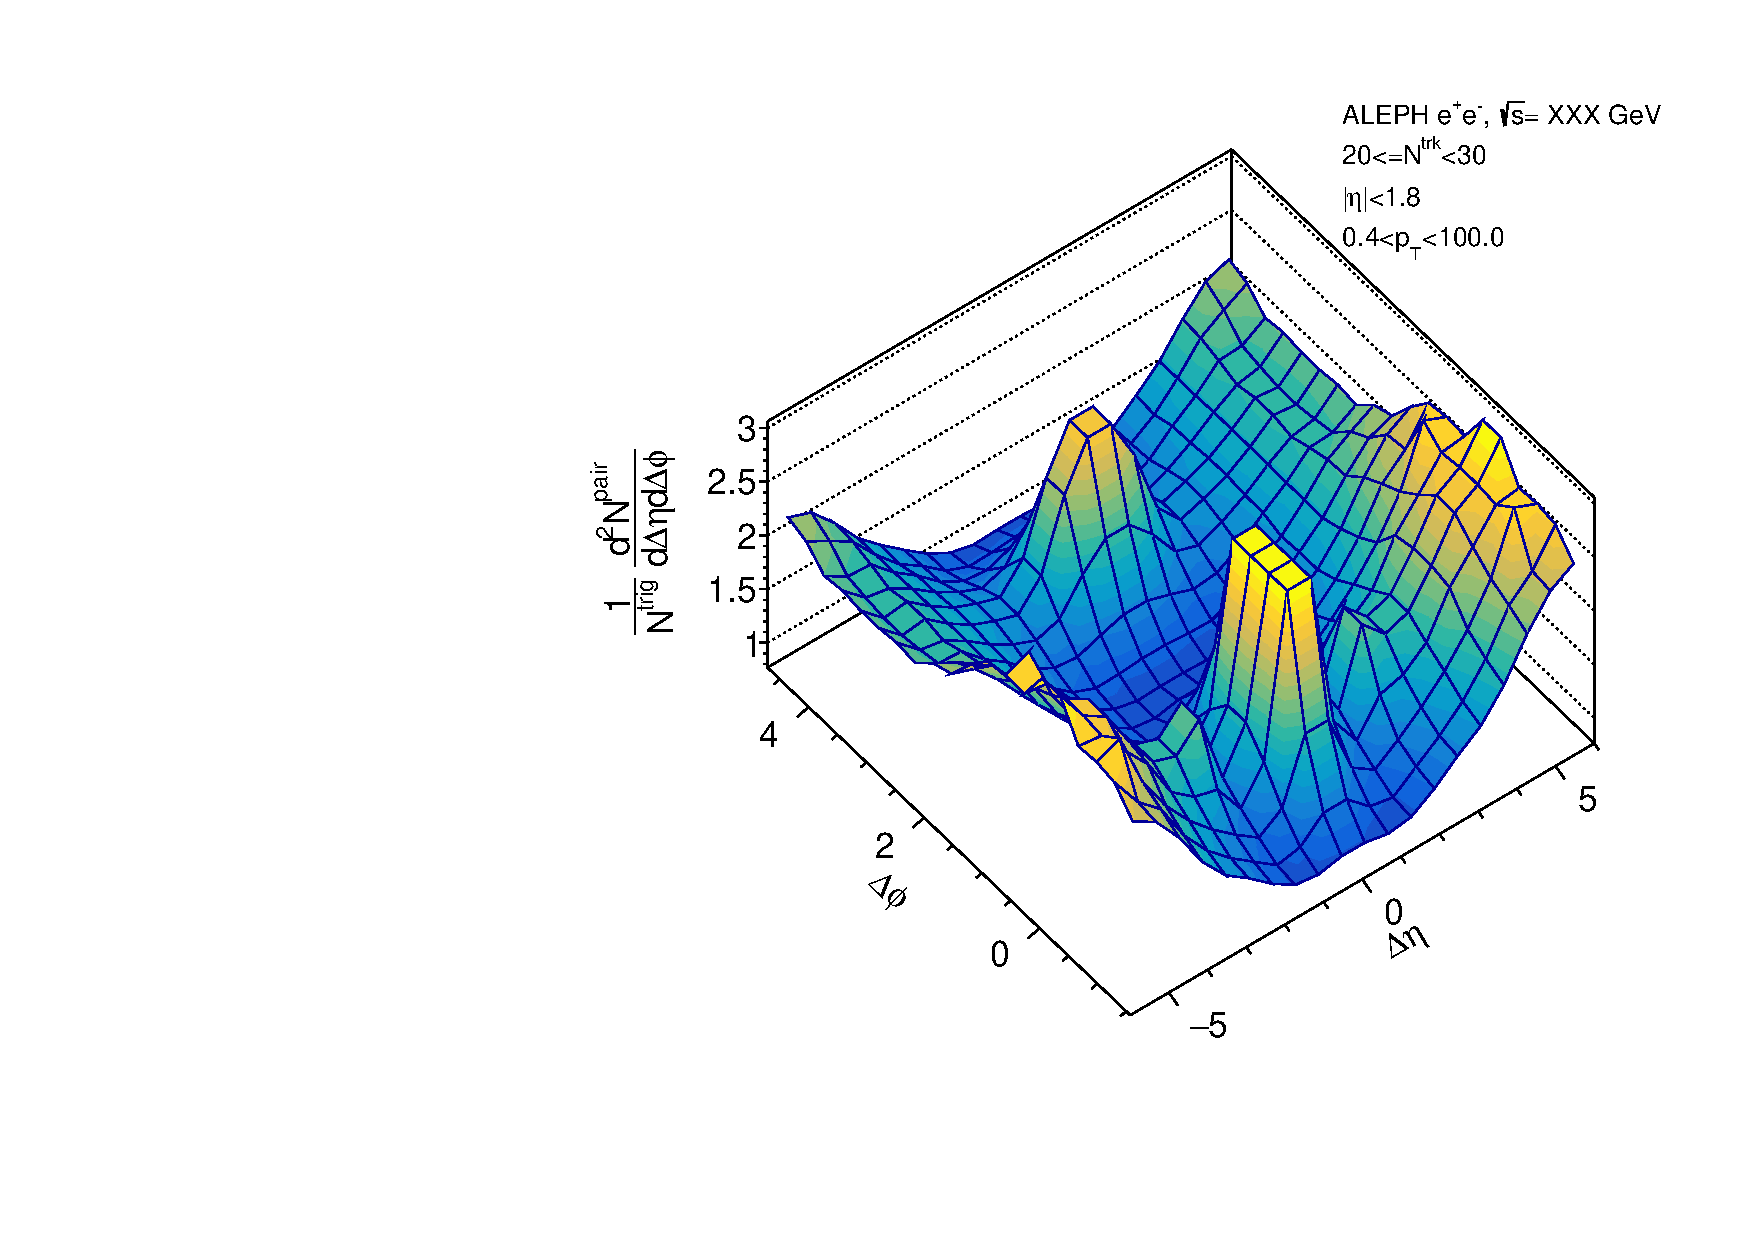
\includegraphics[width=.32\textwidth]{images/TwoParticleCorrelation/LEP2_THRUST/LEP2_THRUST_ratio1_20_30.pdf}}\hfill
\subfloat{\label{sfig:f}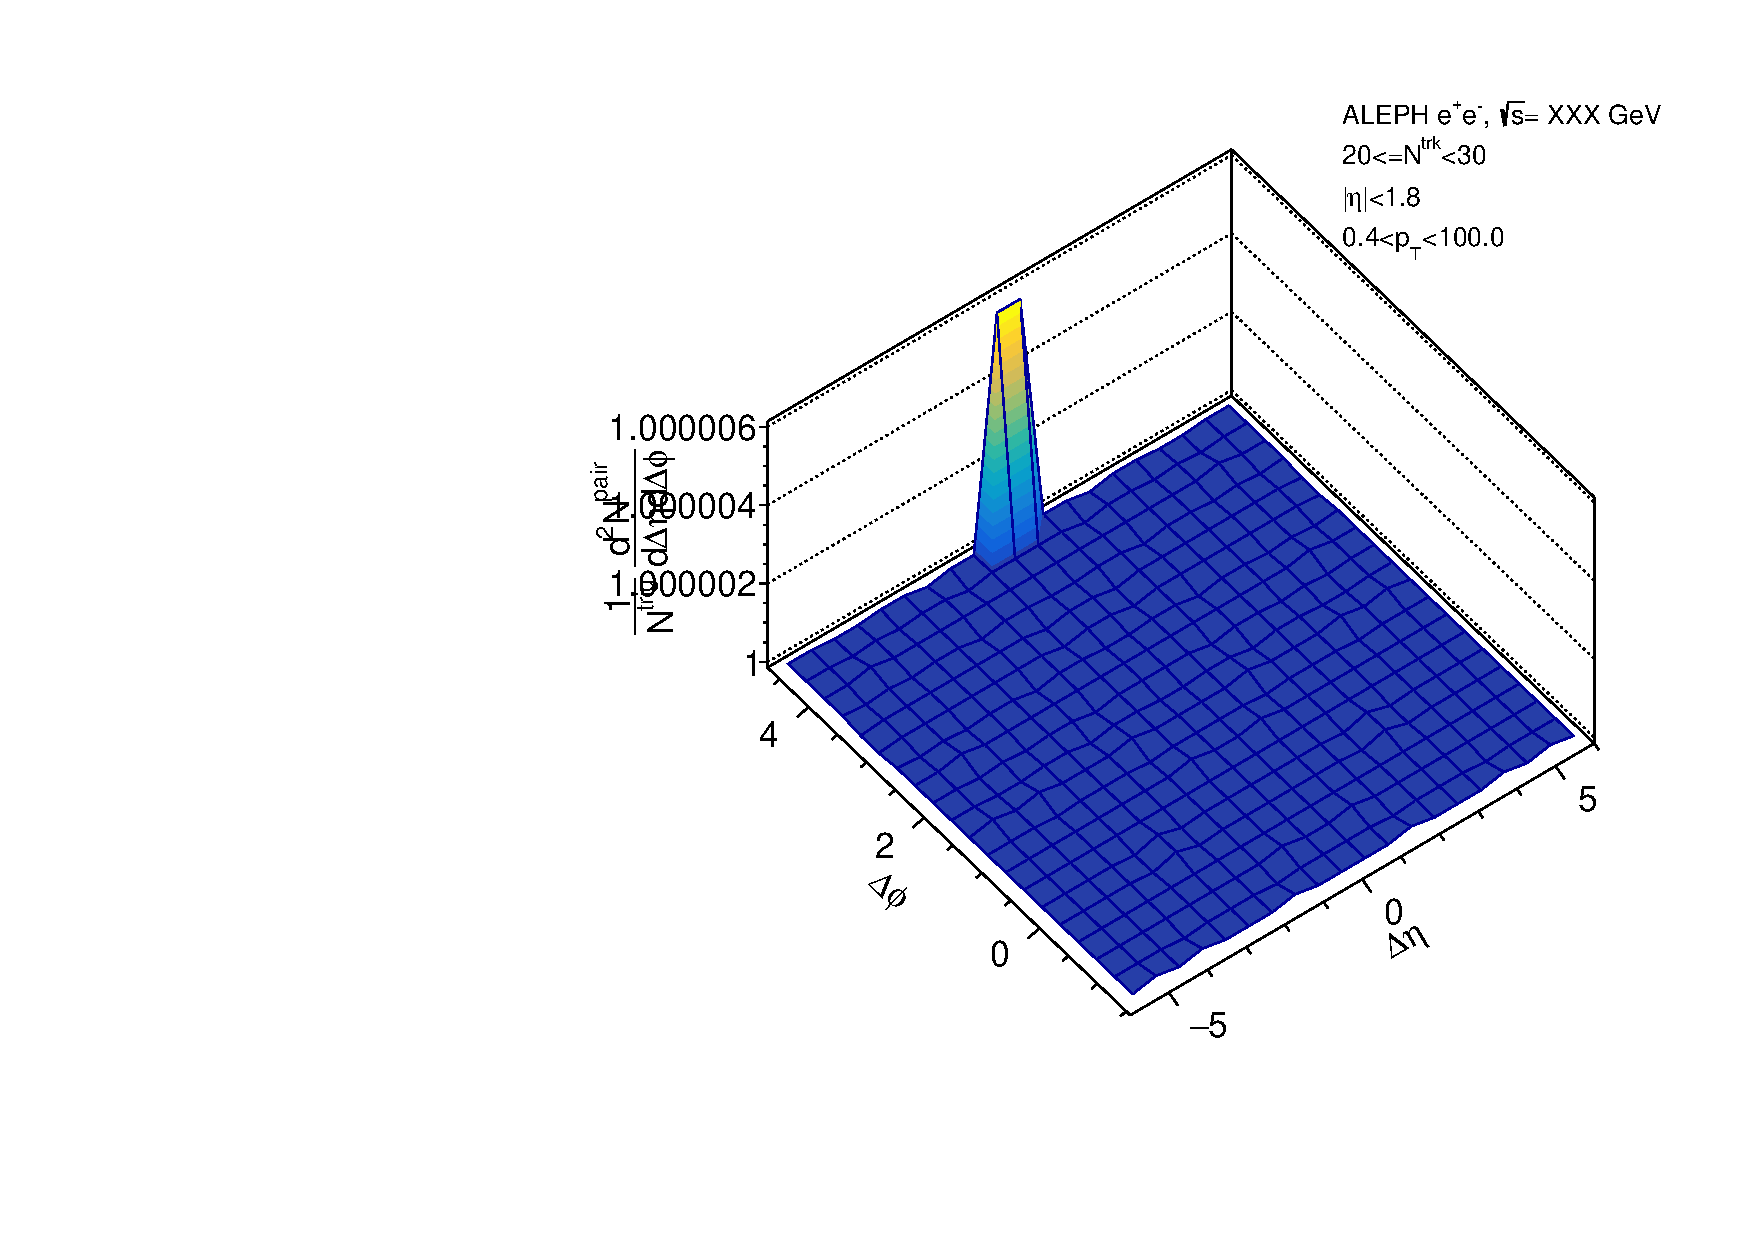
\includegraphics[width=.32\textwidth]{images/TwoParticleCorrelation/LEP2_THRUST/LEP2_THRUST_r_ratio_20_30.pdf}}\hfill
\subfloat{\label{sfig:g}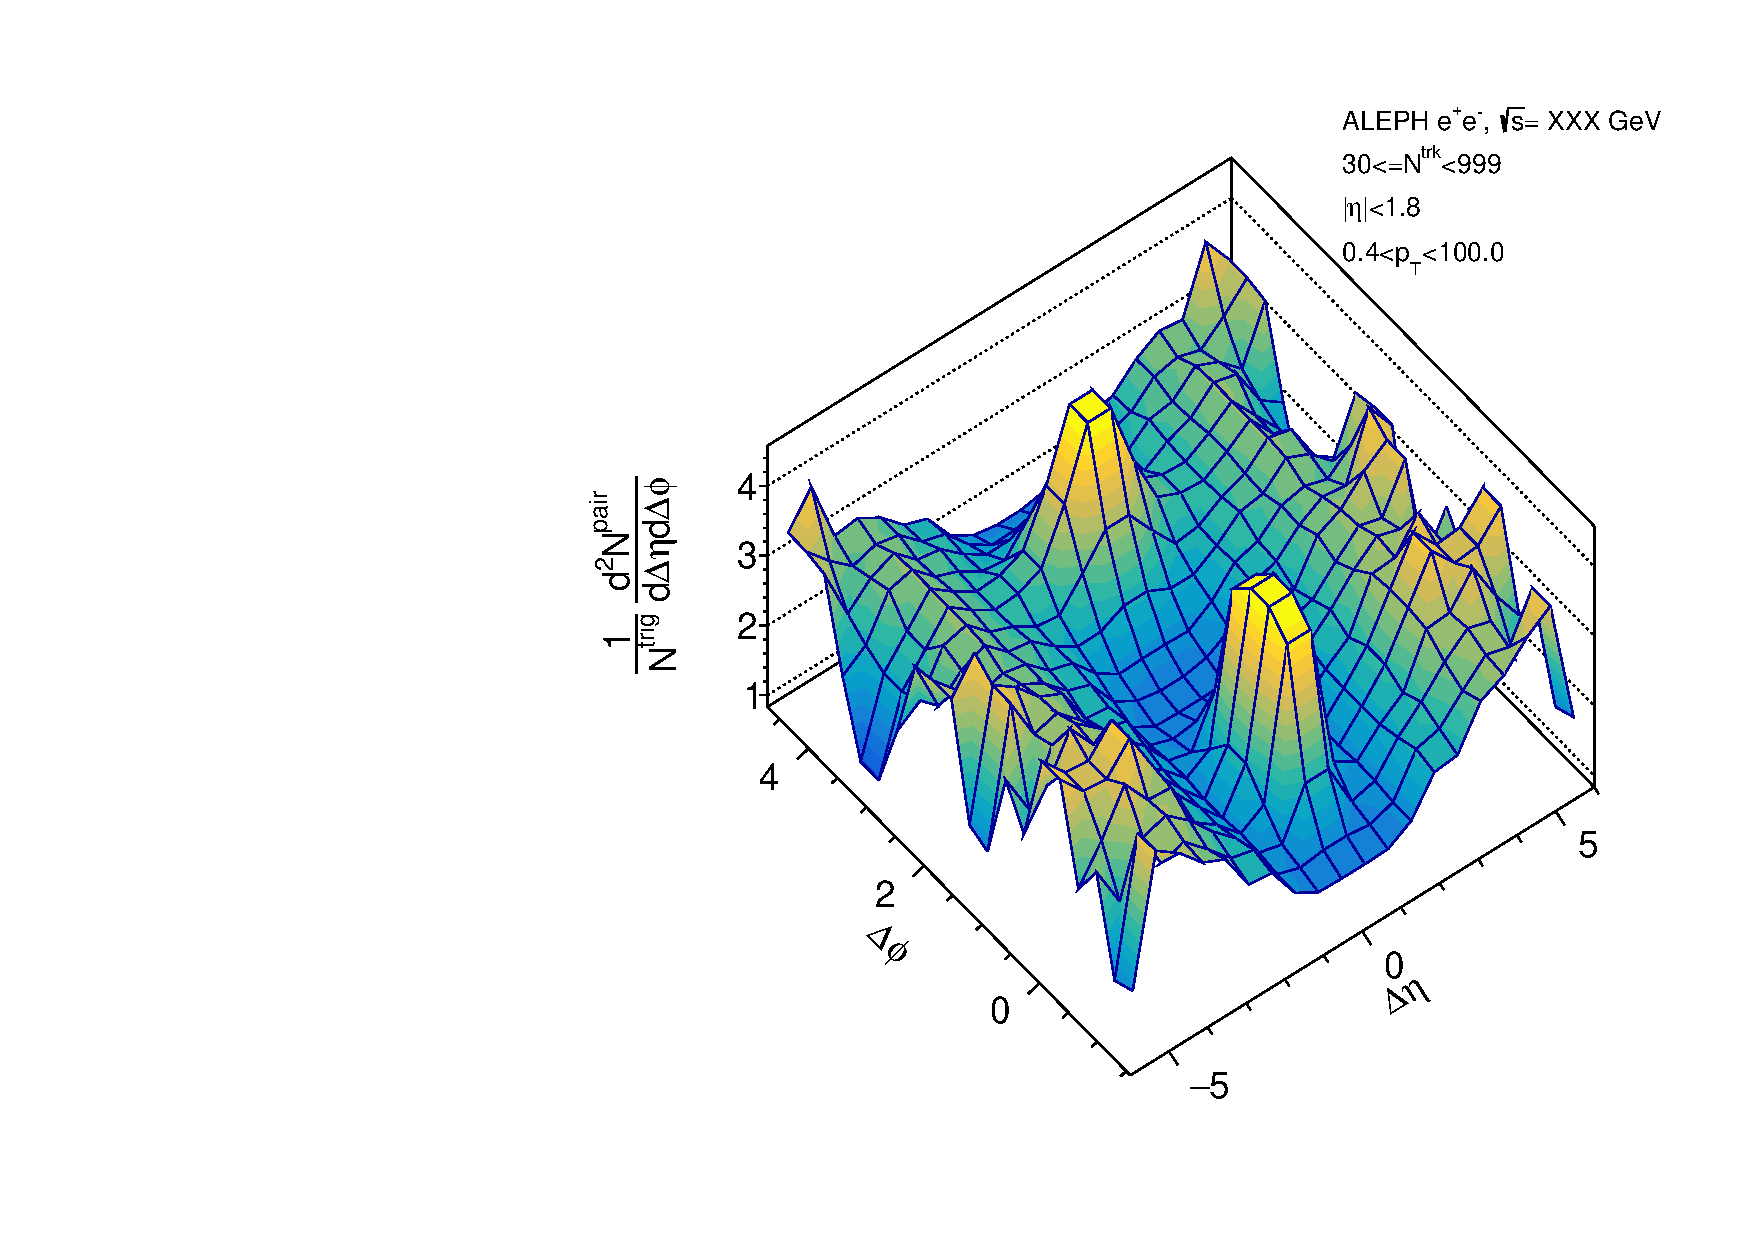
\includegraphics[width=.32\textwidth]{images/TwoParticleCorrelation/LEP2_THRUST/LEP2_THRUST_ratio2_30_999.pdf}}\hfill
\subfloat{\label{sfig:h}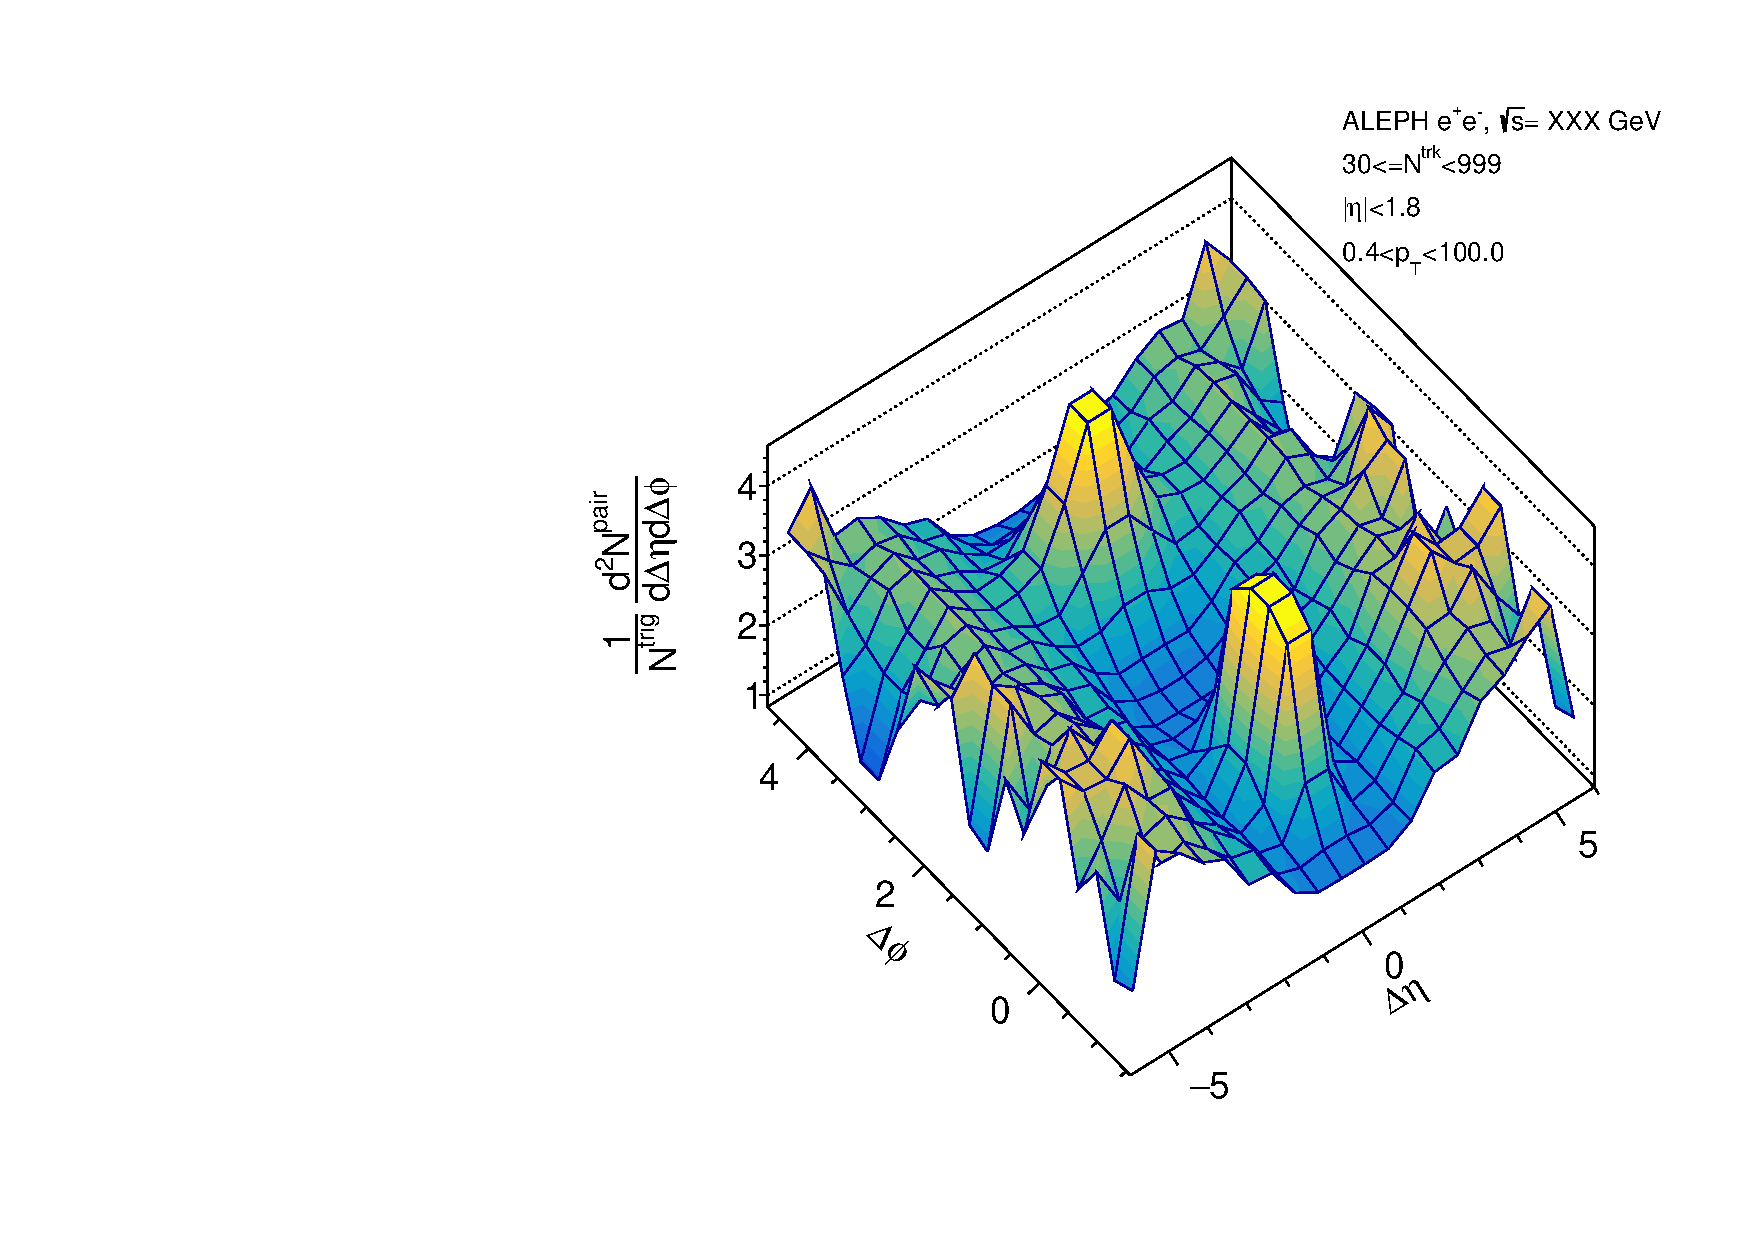
\includegraphics[width=.32\textwidth]{images/TwoParticleCorrelation/LEP2_THRUST/LEP2_THRUST_ratio1_30_999.pdf}}\hfill
\subfloat{\label{sfig:i}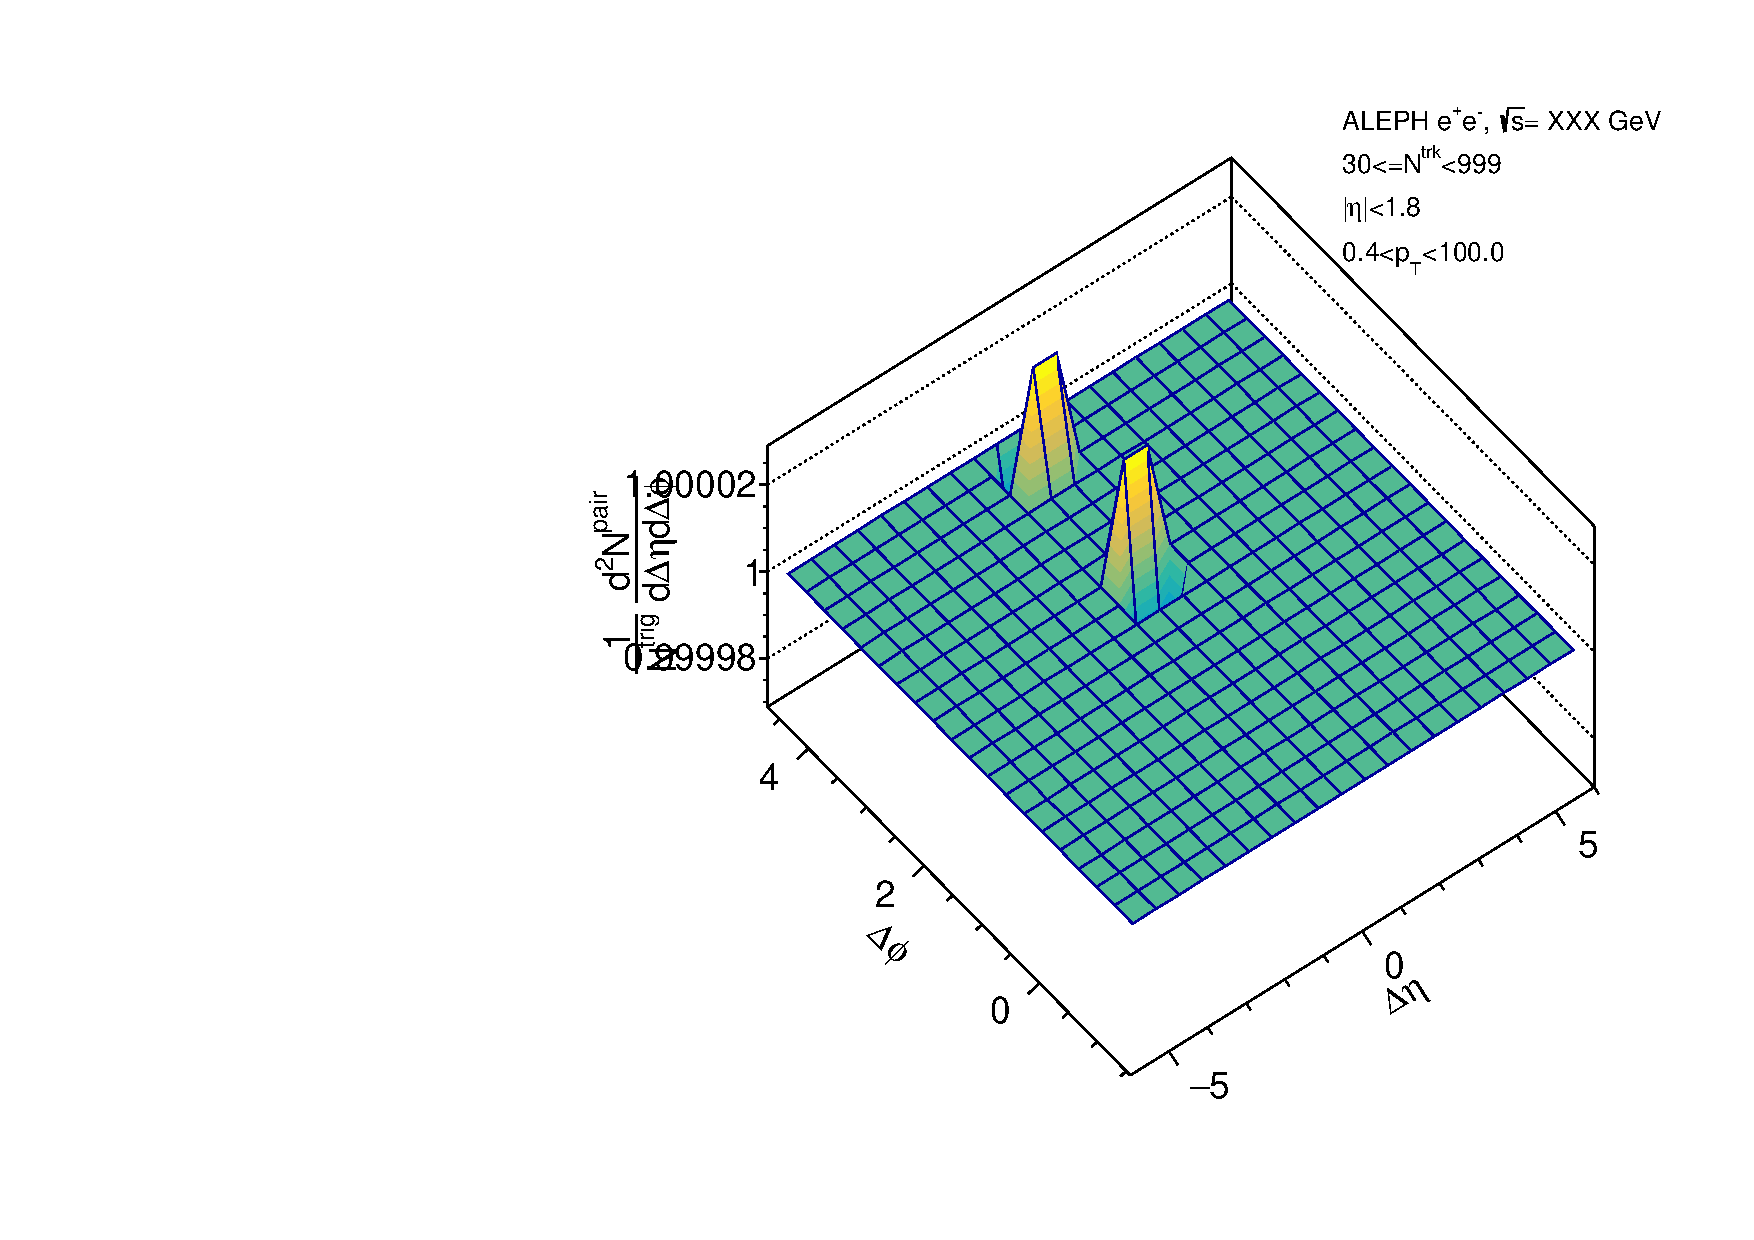
\includegraphics[width=.32\textwidth]{images/TwoParticleCorrelation/LEP2_THRUST/LEP2_THRUST_r_ratio_30_999.pdf}} \\
\caption{Two particle correlation fuctions for the LEP2 data set analyzed in the thrust axis.}
\label{fig:test}
\end{figure}

\begin{figure}[h!]
\centering
\subfloat{\label{sfig:a}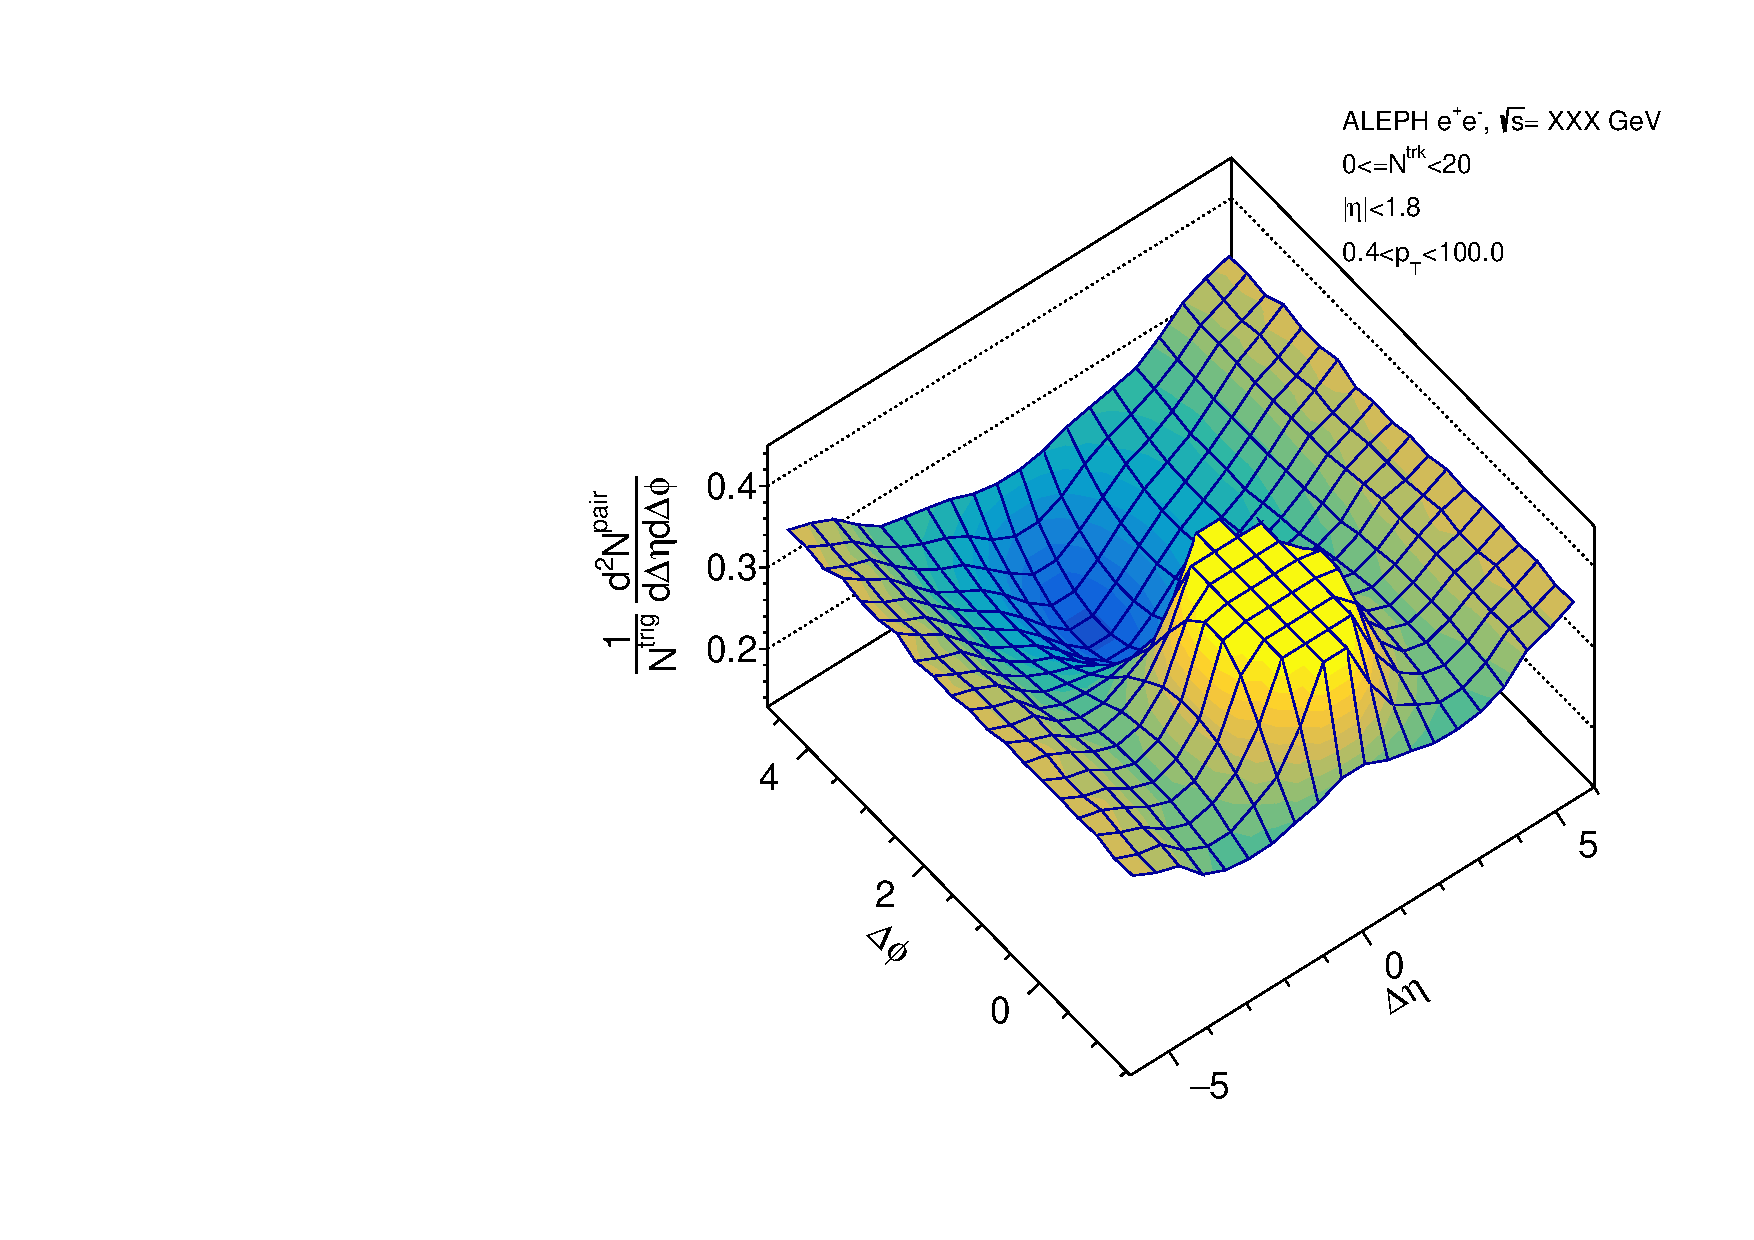
\includegraphics[width=.32\textwidth]{images/TwoParticleCorrelation/LEP2_WTA/LEP2_WTA_ratio2_0_20.pdf}}\hfill
\subfloat{\label{sfig:b}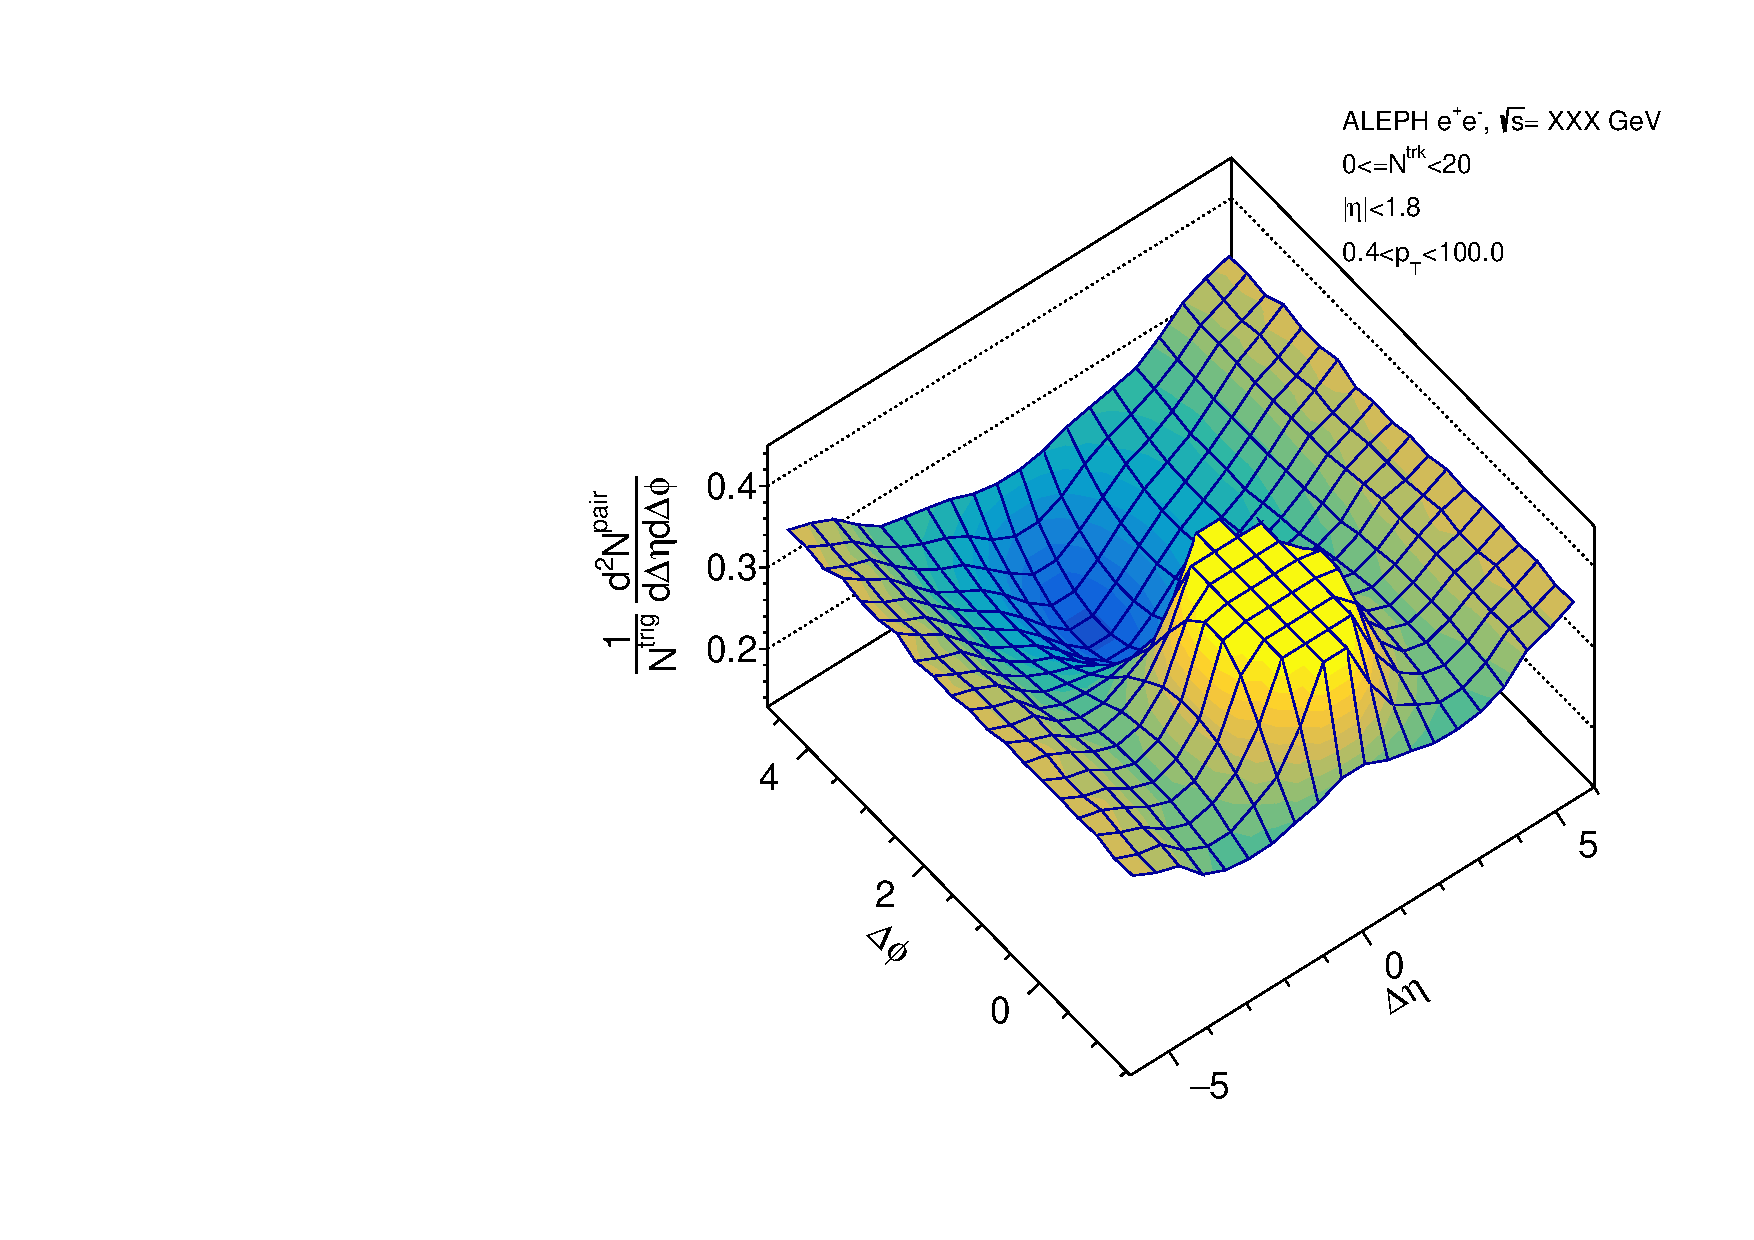
\includegraphics[width=.32\textwidth]{images/TwoParticleCorrelation/LEP2_WTA/LEP2_WTA_ratio1_0_20.pdf}}\hfill
\subfloat{\label{sfig:c}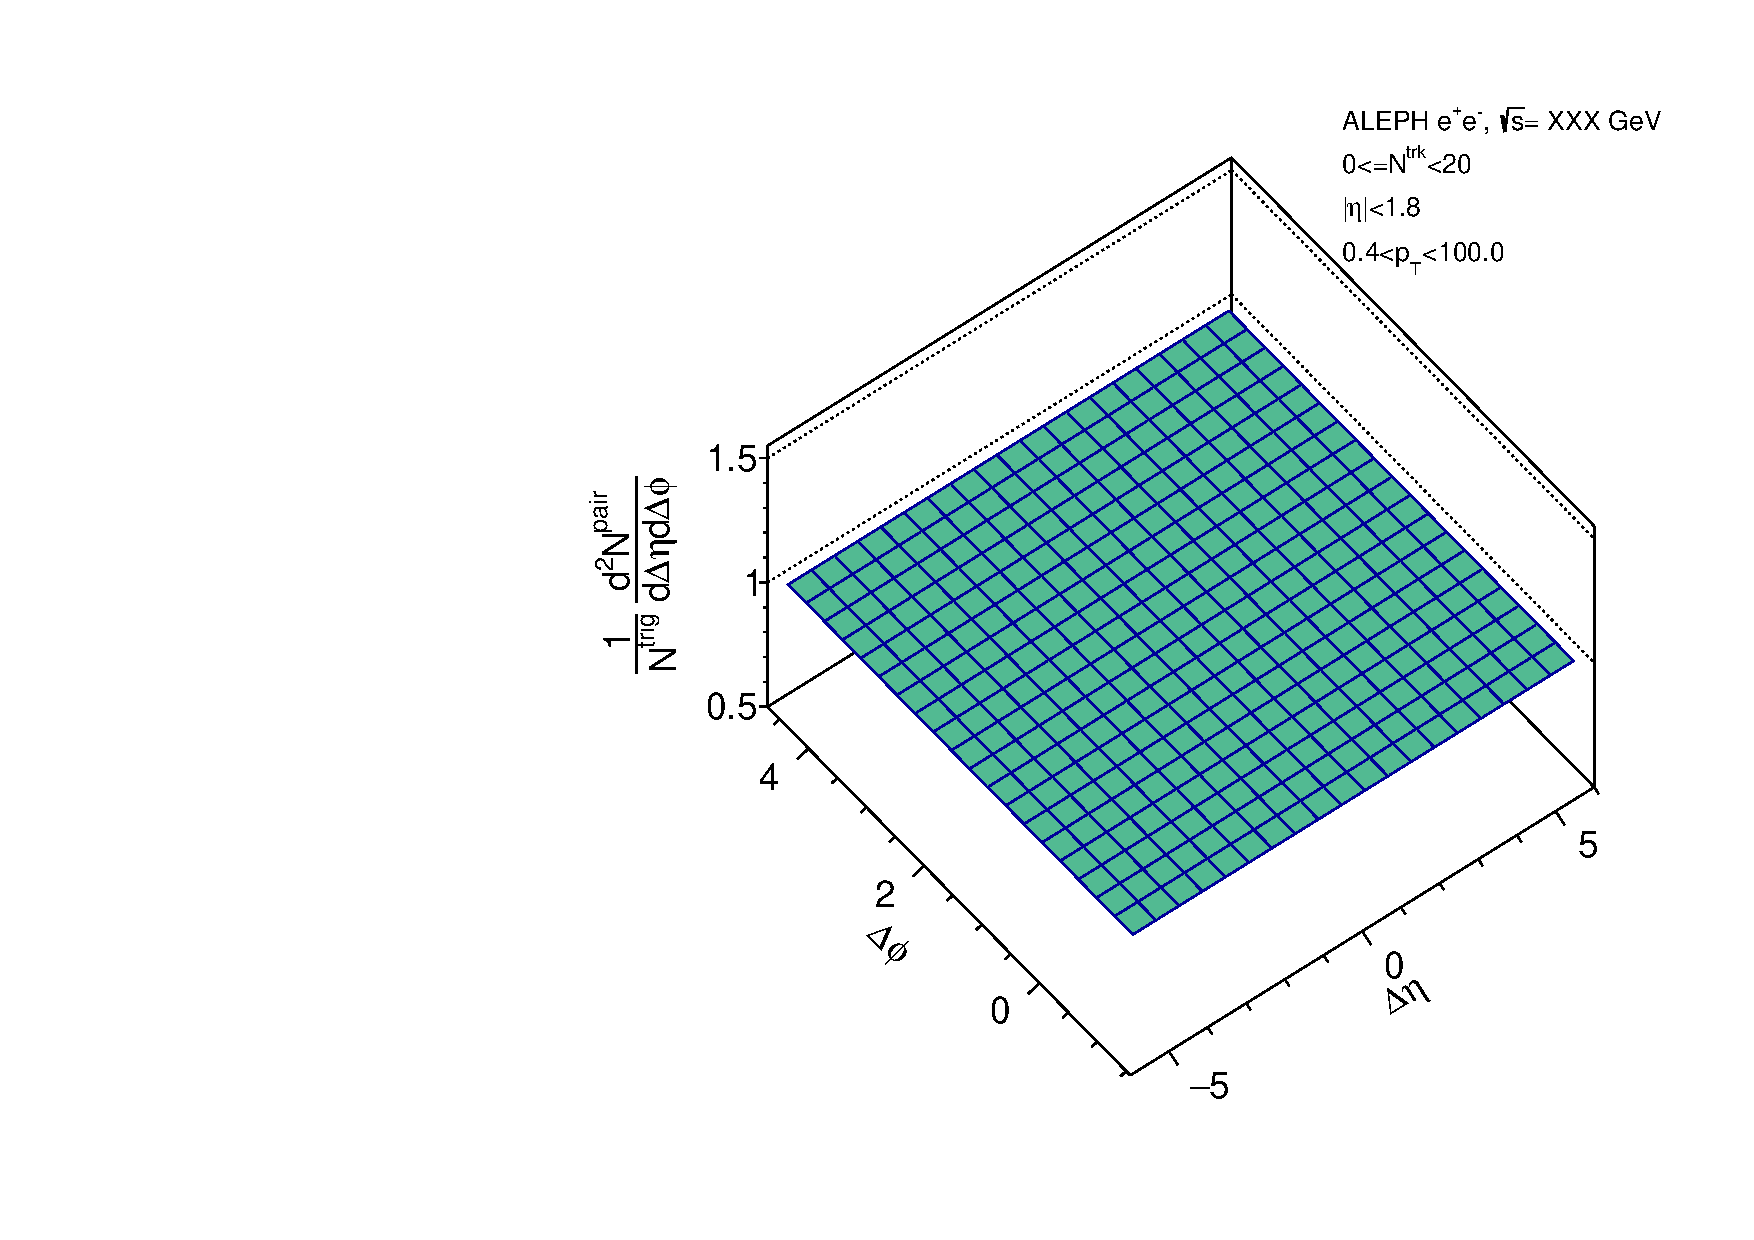
\includegraphics[width=.32\textwidth]{images/TwoParticleCorrelation/LEP2_WTA/LEP2_WTA_r_ratio_0_20.pdf}}\hfill
\subfloat{\label{sfig:d}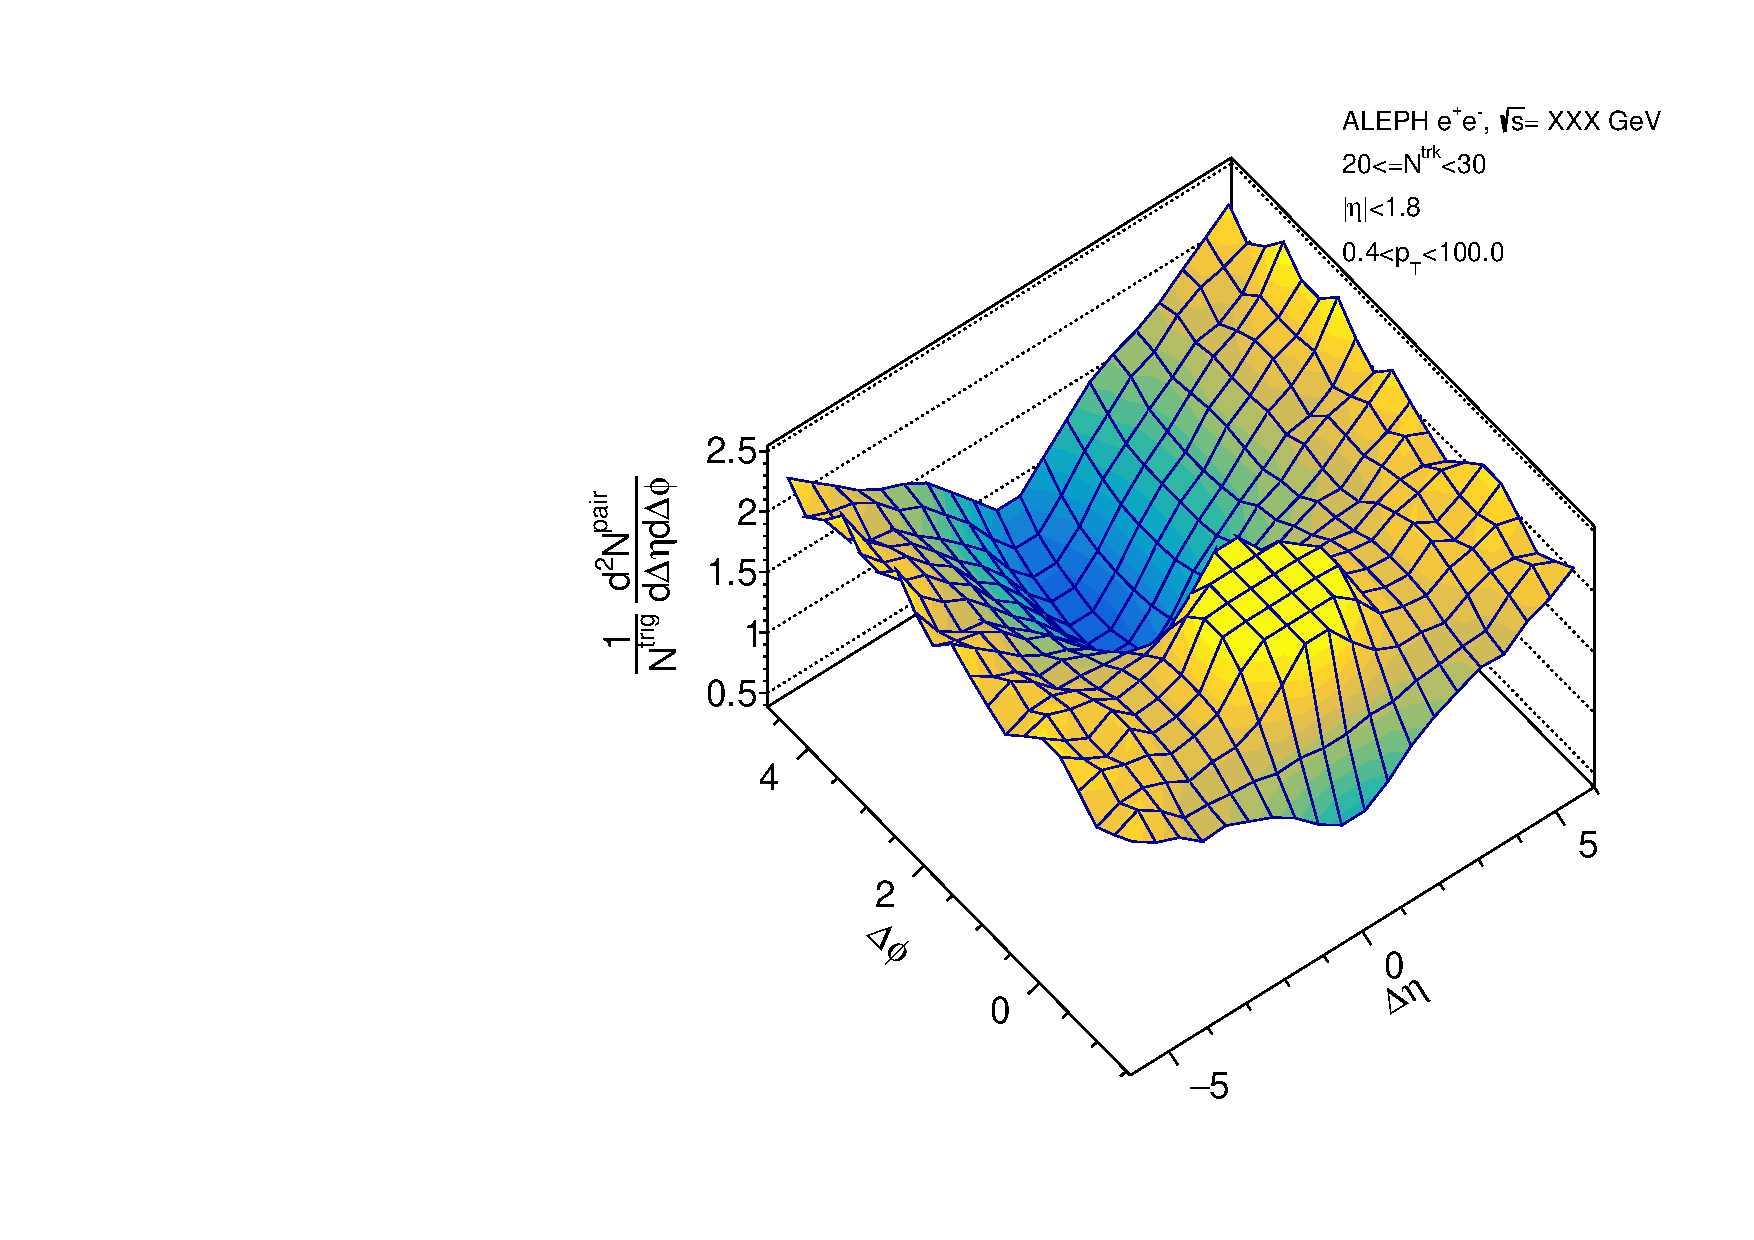
\includegraphics[width=.32\textwidth]{images/TwoParticleCorrelation/LEP2_WTA/LEP2_WTA_ratio2_20_30.pdf}}\hfill
\subfloat{\label{sfig:e}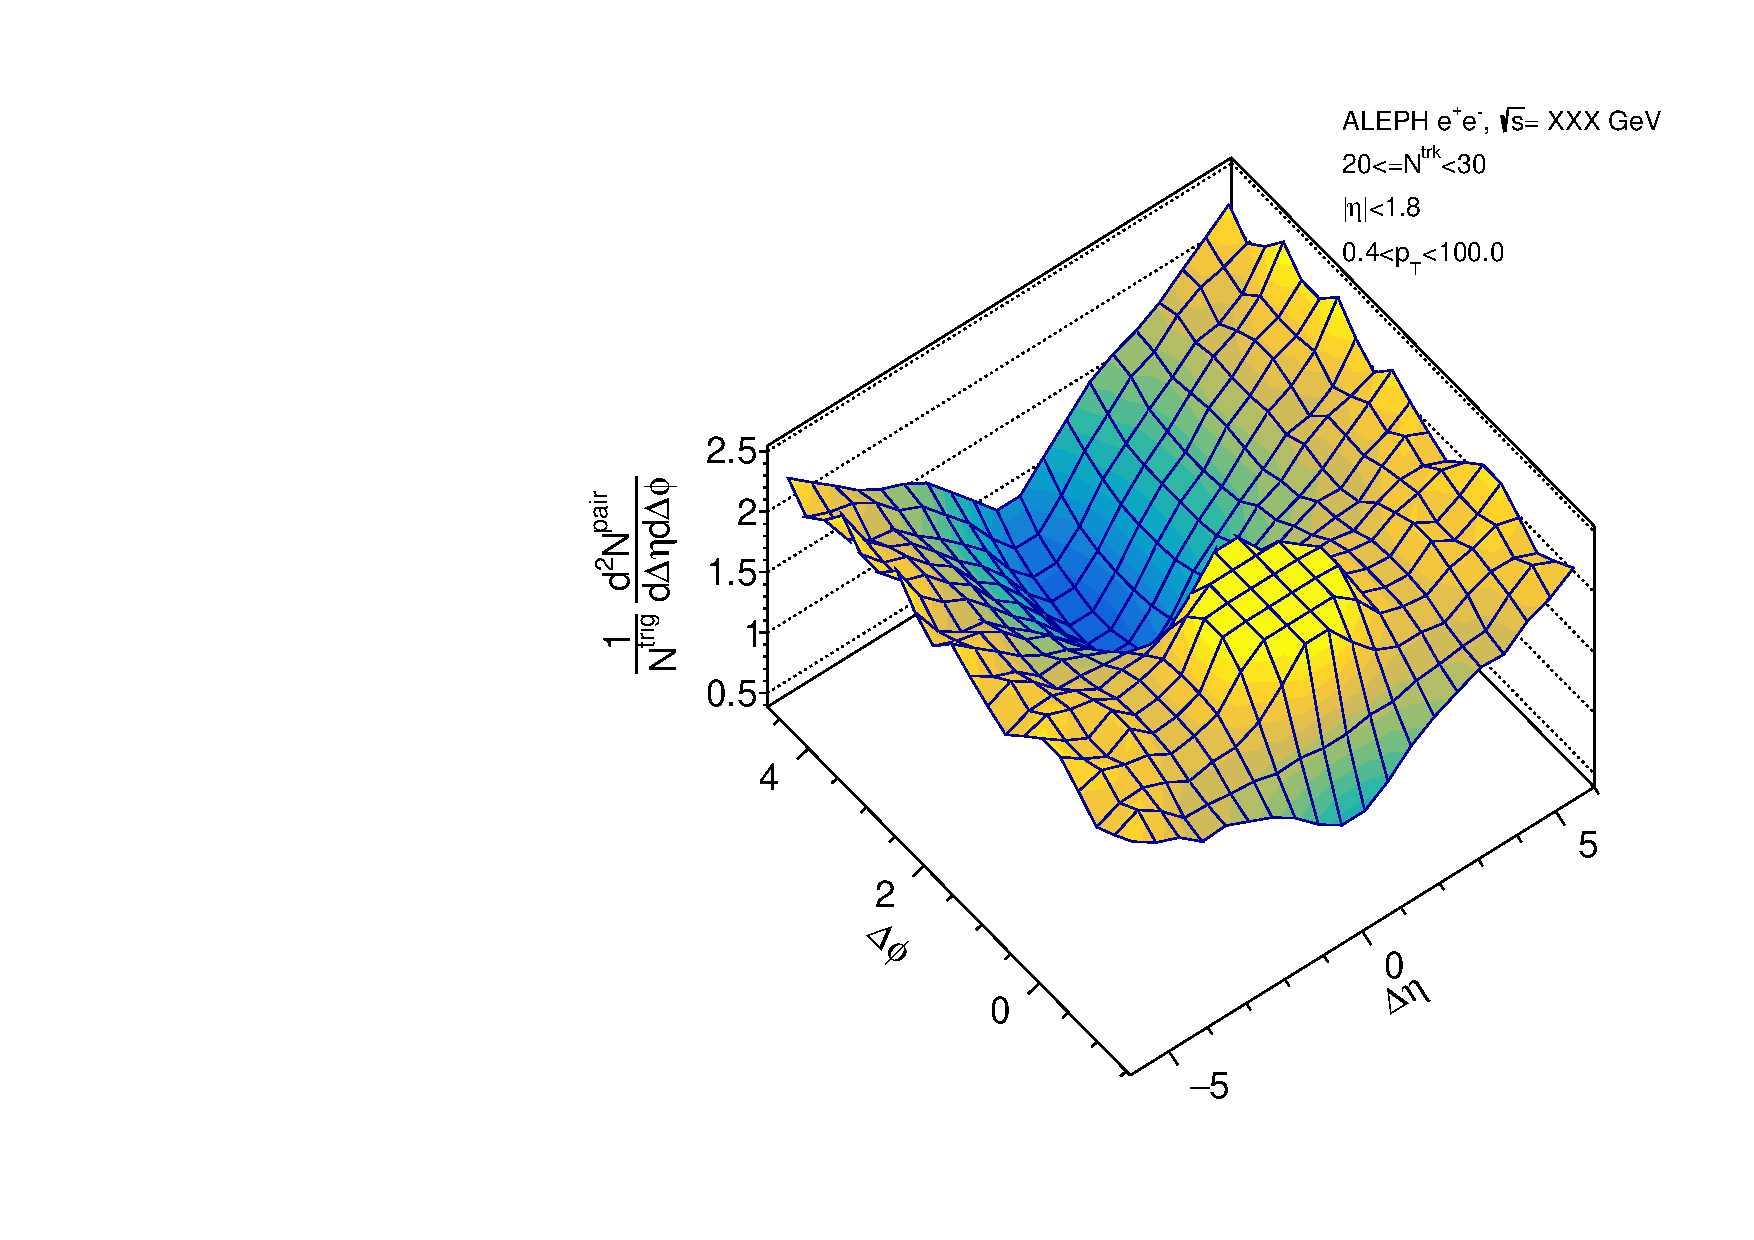
\includegraphics[width=.32\textwidth]{images/TwoParticleCorrelation/LEP2_WTA/LEP2_WTA_ratio1_20_30.pdf}}\hfill
\subfloat{\label{sfig:f}\includegraphics[width=.32\textwidth]{images/TwoParticleCorrelation/LEP2_WTA/LEP2_WTA_r_ratio_20_30.pdf}}\hfill
\subfloat{\label{sfig:g}\includegraphics[width=.32\textwidth]{images/TwoParticleCorrelation/LEP2_WTA/LEP2_WTA_ratio2_30_999.pdf}}\hfill
\subfloat{\label{sfig:h}\includegraphics[width=.32\textwidth]{images/TwoParticleCorrelation/LEP2_WTA/LEP2_WTA_ratio1_30_999.pdf}}\hfill
\subfloat{\label{sfig:i}\includegraphics[width=.32\textwidth]{images/TwoParticleCorrelation/LEP2_WTA/LEP2_WTA_r_ratio_30_999.pdf}} \\
\caption{Two particle correlation fuctions for the LEP2 data set analyzed in the WTA axis.}
\label{fig:test}
\end{figure}

%%%%%%%%%%% PYTHIA8 %%%%%%%%%%%
\begin{figure}[h!]
\centering
\subfloat{\label{sfig:a}\includegraphics[width=.32\textwidth]{images/TwoParticleCorrelation/PYTHIA8_WTA/PYTHIA8_WTA_ratio2_0_20.pdf}}\hfill
\subfloat{\label{sfig:b}\includegraphics[width=.32\textwidth]{images/TwoParticleCorrelation/PYTHIA8_WTA/PYTHIA8_WTA_ratio1_0_20.pdf}}\hfill
\subfloat{\label{sfig:c}\includegraphics[width=.32\textwidth]{images/TwoParticleCorrelation/PYTHIA8_WTA/PYTHIA8_WTA_r_ratio_0_20.pdf}}\hfill
\subfloat{\label{sfig:d}\includegraphics[width=.32\textwidth]{images/TwoParticleCorrelation/PYTHIA8_WTA/PYTHIA8_WTA_ratio2_20_30.pdf}}\hfill
\subfloat{\label{sfig:e}\includegraphics[width=.32\textwidth]{images/TwoParticleCorrelation/PYTHIA8_WTA/PYTHIA8_WTA_ratio1_20_30.pdf}}\hfill
\subfloat{\label{sfig:f}\includegraphics[width=.32\textwidth]{images/TwoParticleCorrelation/PYTHIA8_WTA/PYTHIA8_WTA_r_ratio_20_30.pdf}}\hfill
\subfloat{\label{sfig:g}\includegraphics[width=.32\textwidth]{images/TwoParticleCorrelation/PYTHIA8_WTA/PYTHIA8_WTA_ratio2_30_999.pdf}}\hfill
\subfloat{\label{sfig:h}\includegraphics[width=.32\textwidth]{images/TwoParticleCorrelation/PYTHIA8_WTA/PYTHIA8_WTA_ratio1_30_999.pdf}}\hfill
\subfloat{\label{sfig:i}\includegraphics[width=.32\textwidth]{images/TwoParticleCorrelation/PYTHIA8_WTA/PYTHIA8_WTA_r_ratio_30_999.pdf}} \\
\caption{Two particle correlation fuctions for the PYTHIA8 data set analyzed in the WTA axis.}
\label{fig:test}
\end{figure}


%%%%%%%%%%% PYTHIA8 Rope Walk %%%%%%%%%%%
\begin{figure}[h!]
\centering
\subfloat{\label{sfig:a}\includegraphics[width=.32\textwidth]{images/TwoParticleCorrelation/PYTHIA8_RopeWalk_WTA/PYTHIA8_RopeWalk_WTA_ratio2_0_20.pdf}}\hfill
\subfloat{\label{sfig:b}\includegraphics[width=.32\textwidth]{images/TwoParticleCorrelation/PYTHIA8_RopeWalk_WTA/PYTHIA8_RopeWalk_WTA_ratio1_0_20.pdf}}\hfill
\subfloat{\label{sfig:c}\includegraphics[width=.32\textwidth]{images/TwoParticleCorrelation/PYTHIA8_RopeWalk_WTA/PYTHIA8_RopeWalk_WTA_r_ratio_0_20.pdf}}\hfill
\subfloat{\label{sfig:d}\includegraphics[width=.32\textwidth]{images/TwoParticleCorrelation/PYTHIA8_RopeWalk_WTA/PYTHIA8_RopeWalk_WTA_ratio2_20_30.pdf}}\hfill
\subfloat{\label{sfig:e}\includegraphics[width=.32\textwidth]{images/TwoParticleCorrelation/PYTHIA8_RopeWalk_WTA/PYTHIA8_RopeWalk_WTA_ratio1_20_30.pdf}}\hfill
\subfloat{\label{sfig:f}\includegraphics[width=.32\textwidth]{images/TwoParticleCorrelation/PYTHIA8_RopeWalk_WTA/PYTHIA8_RopeWalk_WTA_r_ratio_20_30.pdf}}\hfill
\subfloat{\label{sfig:g}\includegraphics[width=.32\textwidth]{images/TwoParticleCorrelation/PYTHIA8_RopeWalk_WTA/PYTHIA8_RopeWalk_WTA_ratio2_30_999.pdf}}\hfill
\subfloat{\label{sfig:h}\includegraphics[width=.32\textwidth]{images/TwoParticleCorrelation/PYTHIA8_RopeWalk_WTA/PYTHIA8_RopeWalk_WTA_ratio1_30_999.pdf}}\hfill
\subfloat{\label{sfig:i}\includegraphics[width=.32\textwidth]{images/TwoParticleCorrelation/PYTHIA8_RopeWalk_WTA/PYTHIA8_RopeWalk_WTA_r_ratio_30_999.pdf}} \\
\caption{Two particle correlation fuctions for the PYTHIA8 rope walk data set analyzed in the WTA axis.}
\label{fig:test}
\end{figure}
